\documentclass[11pt]{article}

    \usepackage[breakable]{tcolorbox}
    \usepackage{parskip} % Stop auto-indenting (to mimic markdown behaviour)
    
    \usepackage{iftex}
    \ifPDFTeX
    	\usepackage[T1]{fontenc}
    	\usepackage{mathpazo}
    \else
    	\usepackage{fontspec}
    \fi

    % Basic figure setup, for now with no caption control since it's done
    % automatically by Pandoc (which extracts ![](path) syntax from Markdown).
    \usepackage{graphicx}
    % Maintain compatibility with old templates. Remove in nbconvert 6.0
    \let\Oldincludegraphics\includegraphics
    % Ensure that by default, figures have no caption (until we provide a
    % proper Figure object with a Caption API and a way to capture that
    % in the conversion process - todo).
    \usepackage{caption}
    \DeclareCaptionFormat{nocaption}{}
    \captionsetup{format=nocaption,aboveskip=0pt,belowskip=0pt}

    \usepackage{float}
    \floatplacement{figure}{H} % forces figures to be placed at the correct location
    \usepackage{xcolor} % Allow colors to be defined
    \usepackage{enumerate} % Needed for markdown enumerations to work
    \usepackage{geometry} % Used to adjust the document margins
    \usepackage{amsmath} % Equations
    \usepackage{amssymb} % Equations
    \usepackage{textcomp} % defines textquotesingle
    % Hack from http://tex.stackexchange.com/a/47451/13684:
    \AtBeginDocument{%
        \def\PYZsq{\textquotesingle}% Upright quotes in Pygmentized code
    }
    \usepackage{upquote} % Upright quotes for verbatim code
    \usepackage{eurosym} % defines \euro
    \usepackage[mathletters]{ucs} % Extended unicode (utf-8) support
    \usepackage{fancyvrb} % verbatim replacement that allows latex
    \usepackage{grffile} % extends the file name processing of package graphics 
                         % to support a larger range
    \makeatletter % fix for old versions of grffile with XeLaTeX
    \@ifpackagelater{grffile}{2019/11/01}
    {
      % Do nothing on new versions
    }
    {
      \def\Gread@@xetex#1{%
        \IfFileExists{"\Gin@base".bb}%
        {\Gread@eps{\Gin@base.bb}}%
        {\Gread@@xetex@aux#1}%
      }
    }
    \makeatother
    \usepackage[Export]{adjustbox} % Used to constrain images to a maximum size
    \adjustboxset{max size={0.9\linewidth}{0.9\paperheight}}

    % The hyperref package gives us a pdf with properly built
    % internal navigation ('pdf bookmarks' for the table of contents,
    % internal cross-reference links, web links for URLs, etc.)
    \usepackage{hyperref}
    % The default LaTeX title has an obnoxious amount of whitespace. By default,
    % titling removes some of it. It also provides customization options.
    \usepackage{titling}
    \usepackage{longtable} % longtable support required by pandoc >1.10
    \usepackage{booktabs}  % table support for pandoc > 1.12.2
    \usepackage[inline]{enumitem} % IRkernel/repr support (it uses the enumerate* environment)
    \usepackage[normalem]{ulem} % ulem is needed to support strikethroughs (\sout)
                                % normalem makes italics be italics, not underlines
    \usepackage{mathrsfs}
    

    
    % Colors for the hyperref package
    \definecolor{urlcolor}{rgb}{0,.145,.698}
    \definecolor{linkcolor}{rgb}{.71,0.21,0.01}
    \definecolor{citecolor}{rgb}{.12,.54,.11}

    % ANSI colors
    \definecolor{ansi-black}{HTML}{3E424D}
    \definecolor{ansi-black-intense}{HTML}{282C36}
    \definecolor{ansi-red}{HTML}{E75C58}
    \definecolor{ansi-red-intense}{HTML}{B22B31}
    \definecolor{ansi-green}{HTML}{00A250}
    \definecolor{ansi-green-intense}{HTML}{007427}
    \definecolor{ansi-yellow}{HTML}{DDB62B}
    \definecolor{ansi-yellow-intense}{HTML}{B27D12}
    \definecolor{ansi-blue}{HTML}{208FFB}
    \definecolor{ansi-blue-intense}{HTML}{0065CA}
    \definecolor{ansi-magenta}{HTML}{D160C4}
    \definecolor{ansi-magenta-intense}{HTML}{A03196}
    \definecolor{ansi-cyan}{HTML}{60C6C8}
    \definecolor{ansi-cyan-intense}{HTML}{258F8F}
    \definecolor{ansi-white}{HTML}{C5C1B4}
    \definecolor{ansi-white-intense}{HTML}{A1A6B2}
    \definecolor{ansi-default-inverse-fg}{HTML}{FFFFFF}
    \definecolor{ansi-default-inverse-bg}{HTML}{000000}

    % common color for the border for error outputs.
    \definecolor{outerrorbackground}{HTML}{FFDFDF}

    % commands and environments needed by pandoc snippets
    % extracted from the output of `pandoc -s`
    \providecommand{\tightlist}{%
      \setlength{\itemsep}{0pt}\setlength{\parskip}{0pt}}
    \DefineVerbatimEnvironment{Highlighting}{Verbatim}{commandchars=\\\{\}}
    % Add ',fontsize=\small' for more characters per line
    \newenvironment{Shaded}{}{}
    \newcommand{\KeywordTok}[1]{\textcolor[rgb]{0.00,0.44,0.13}{\textbf{{#1}}}}
    \newcommand{\DataTypeTok}[1]{\textcolor[rgb]{0.56,0.13,0.00}{{#1}}}
    \newcommand{\DecValTok}[1]{\textcolor[rgb]{0.25,0.63,0.44}{{#1}}}
    \newcommand{\BaseNTok}[1]{\textcolor[rgb]{0.25,0.63,0.44}{{#1}}}
    \newcommand{\FloatTok}[1]{\textcolor[rgb]{0.25,0.63,0.44}{{#1}}}
    \newcommand{\CharTok}[1]{\textcolor[rgb]{0.25,0.44,0.63}{{#1}}}
    \newcommand{\StringTok}[1]{\textcolor[rgb]{0.25,0.44,0.63}{{#1}}}
    \newcommand{\CommentTok}[1]{\textcolor[rgb]{0.38,0.63,0.69}{\textit{{#1}}}}
    \newcommand{\OtherTok}[1]{\textcolor[rgb]{0.00,0.44,0.13}{{#1}}}
    \newcommand{\AlertTok}[1]{\textcolor[rgb]{1.00,0.00,0.00}{\textbf{{#1}}}}
    \newcommand{\FunctionTok}[1]{\textcolor[rgb]{0.02,0.16,0.49}{{#1}}}
    \newcommand{\RegionMarkerTok}[1]{{#1}}
    \newcommand{\ErrorTok}[1]{\textcolor[rgb]{1.00,0.00,0.00}{\textbf{{#1}}}}
    \newcommand{\NormalTok}[1]{{#1}}
    
    % Additional commands for more recent versions of Pandoc
    \newcommand{\ConstantTok}[1]{\textcolor[rgb]{0.53,0.00,0.00}{{#1}}}
    \newcommand{\SpecialCharTok}[1]{\textcolor[rgb]{0.25,0.44,0.63}{{#1}}}
    \newcommand{\VerbatimStringTok}[1]{\textcolor[rgb]{0.25,0.44,0.63}{{#1}}}
    \newcommand{\SpecialStringTok}[1]{\textcolor[rgb]{0.73,0.40,0.53}{{#1}}}
    \newcommand{\ImportTok}[1]{{#1}}
    \newcommand{\DocumentationTok}[1]{\textcolor[rgb]{0.73,0.13,0.13}{\textit{{#1}}}}
    \newcommand{\AnnotationTok}[1]{\textcolor[rgb]{0.38,0.63,0.69}{\textbf{\textit{{#1}}}}}
    \newcommand{\CommentVarTok}[1]{\textcolor[rgb]{0.38,0.63,0.69}{\textbf{\textit{{#1}}}}}
    \newcommand{\VariableTok}[1]{\textcolor[rgb]{0.10,0.09,0.49}{{#1}}}
    \newcommand{\ControlFlowTok}[1]{\textcolor[rgb]{0.00,0.44,0.13}{\textbf{{#1}}}}
    \newcommand{\OperatorTok}[1]{\textcolor[rgb]{0.40,0.40,0.40}{{#1}}}
    \newcommand{\BuiltInTok}[1]{{#1}}
    \newcommand{\ExtensionTok}[1]{{#1}}
    \newcommand{\PreprocessorTok}[1]{\textcolor[rgb]{0.74,0.48,0.00}{{#1}}}
    \newcommand{\AttributeTok}[1]{\textcolor[rgb]{0.49,0.56,0.16}{{#1}}}
    \newcommand{\InformationTok}[1]{\textcolor[rgb]{0.38,0.63,0.69}{\textbf{\textit{{#1}}}}}
    \newcommand{\WarningTok}[1]{\textcolor[rgb]{0.38,0.63,0.69}{\textbf{\textit{{#1}}}}}
    
    
    % Define a nice break command that doesn't care if a line doesn't already
    % exist.
    \def\br{\hspace*{\fill} \\* }
    % Math Jax compatibility definitions
    \def\gt{>}
    \def\lt{<}
    \let\Oldtex\TeX
    \let\Oldlatex\LaTeX
    \renewcommand{\TeX}{\textrm{\Oldtex}}
    \renewcommand{\LaTeX}{\textrm{\Oldlatex}}
    % Document parameters
    % Document title
    \title{Raport}
    
    
    
    
    
% Pygments definitions
\makeatletter
\def\PY@reset{\let\PY@it=\relax \let\PY@bf=\relax%
    \let\PY@ul=\relax \let\PY@tc=\relax%
    \let\PY@bc=\relax \let\PY@ff=\relax}
\def\PY@tok#1{\csname PY@tok@#1\endcsname}
\def\PY@toks#1+{\ifx\relax#1\empty\else%
    \PY@tok{#1}\expandafter\PY@toks\fi}
\def\PY@do#1{\PY@bc{\PY@tc{\PY@ul{%
    \PY@it{\PY@bf{\PY@ff{#1}}}}}}}
\def\PY#1#2{\PY@reset\PY@toks#1+\relax+\PY@do{#2}}

\expandafter\def\csname PY@tok@w\endcsname{\def\PY@tc##1{\textcolor[rgb]{0.73,0.73,0.73}{##1}}}
\expandafter\def\csname PY@tok@c\endcsname{\let\PY@it=\textit\def\PY@tc##1{\textcolor[rgb]{0.25,0.50,0.50}{##1}}}
\expandafter\def\csname PY@tok@cp\endcsname{\def\PY@tc##1{\textcolor[rgb]{0.74,0.48,0.00}{##1}}}
\expandafter\def\csname PY@tok@k\endcsname{\let\PY@bf=\textbf\def\PY@tc##1{\textcolor[rgb]{0.00,0.50,0.00}{##1}}}
\expandafter\def\csname PY@tok@kp\endcsname{\def\PY@tc##1{\textcolor[rgb]{0.00,0.50,0.00}{##1}}}
\expandafter\def\csname PY@tok@kt\endcsname{\def\PY@tc##1{\textcolor[rgb]{0.69,0.00,0.25}{##1}}}
\expandafter\def\csname PY@tok@o\endcsname{\def\PY@tc##1{\textcolor[rgb]{0.40,0.40,0.40}{##1}}}
\expandafter\def\csname PY@tok@ow\endcsname{\let\PY@bf=\textbf\def\PY@tc##1{\textcolor[rgb]{0.67,0.13,1.00}{##1}}}
\expandafter\def\csname PY@tok@nb\endcsname{\def\PY@tc##1{\textcolor[rgb]{0.00,0.50,0.00}{##1}}}
\expandafter\def\csname PY@tok@nf\endcsname{\def\PY@tc##1{\textcolor[rgb]{0.00,0.00,1.00}{##1}}}
\expandafter\def\csname PY@tok@nc\endcsname{\let\PY@bf=\textbf\def\PY@tc##1{\textcolor[rgb]{0.00,0.00,1.00}{##1}}}
\expandafter\def\csname PY@tok@nn\endcsname{\let\PY@bf=\textbf\def\PY@tc##1{\textcolor[rgb]{0.00,0.00,1.00}{##1}}}
\expandafter\def\csname PY@tok@ne\endcsname{\let\PY@bf=\textbf\def\PY@tc##1{\textcolor[rgb]{0.82,0.25,0.23}{##1}}}
\expandafter\def\csname PY@tok@nv\endcsname{\def\PY@tc##1{\textcolor[rgb]{0.10,0.09,0.49}{##1}}}
\expandafter\def\csname PY@tok@no\endcsname{\def\PY@tc##1{\textcolor[rgb]{0.53,0.00,0.00}{##1}}}
\expandafter\def\csname PY@tok@nl\endcsname{\def\PY@tc##1{\textcolor[rgb]{0.63,0.63,0.00}{##1}}}
\expandafter\def\csname PY@tok@ni\endcsname{\let\PY@bf=\textbf\def\PY@tc##1{\textcolor[rgb]{0.60,0.60,0.60}{##1}}}
\expandafter\def\csname PY@tok@na\endcsname{\def\PY@tc##1{\textcolor[rgb]{0.49,0.56,0.16}{##1}}}
\expandafter\def\csname PY@tok@nt\endcsname{\let\PY@bf=\textbf\def\PY@tc##1{\textcolor[rgb]{0.00,0.50,0.00}{##1}}}
\expandafter\def\csname PY@tok@nd\endcsname{\def\PY@tc##1{\textcolor[rgb]{0.67,0.13,1.00}{##1}}}
\expandafter\def\csname PY@tok@s\endcsname{\def\PY@tc##1{\textcolor[rgb]{0.73,0.13,0.13}{##1}}}
\expandafter\def\csname PY@tok@sd\endcsname{\let\PY@it=\textit\def\PY@tc##1{\textcolor[rgb]{0.73,0.13,0.13}{##1}}}
\expandafter\def\csname PY@tok@si\endcsname{\let\PY@bf=\textbf\def\PY@tc##1{\textcolor[rgb]{0.73,0.40,0.53}{##1}}}
\expandafter\def\csname PY@tok@se\endcsname{\let\PY@bf=\textbf\def\PY@tc##1{\textcolor[rgb]{0.73,0.40,0.13}{##1}}}
\expandafter\def\csname PY@tok@sr\endcsname{\def\PY@tc##1{\textcolor[rgb]{0.73,0.40,0.53}{##1}}}
\expandafter\def\csname PY@tok@ss\endcsname{\def\PY@tc##1{\textcolor[rgb]{0.10,0.09,0.49}{##1}}}
\expandafter\def\csname PY@tok@sx\endcsname{\def\PY@tc##1{\textcolor[rgb]{0.00,0.50,0.00}{##1}}}
\expandafter\def\csname PY@tok@m\endcsname{\def\PY@tc##1{\textcolor[rgb]{0.40,0.40,0.40}{##1}}}
\expandafter\def\csname PY@tok@gh\endcsname{\let\PY@bf=\textbf\def\PY@tc##1{\textcolor[rgb]{0.00,0.00,0.50}{##1}}}
\expandafter\def\csname PY@tok@gu\endcsname{\let\PY@bf=\textbf\def\PY@tc##1{\textcolor[rgb]{0.50,0.00,0.50}{##1}}}
\expandafter\def\csname PY@tok@gd\endcsname{\def\PY@tc##1{\textcolor[rgb]{0.63,0.00,0.00}{##1}}}
\expandafter\def\csname PY@tok@gi\endcsname{\def\PY@tc##1{\textcolor[rgb]{0.00,0.63,0.00}{##1}}}
\expandafter\def\csname PY@tok@gr\endcsname{\def\PY@tc##1{\textcolor[rgb]{1.00,0.00,0.00}{##1}}}
\expandafter\def\csname PY@tok@ge\endcsname{\let\PY@it=\textit}
\expandafter\def\csname PY@tok@gs\endcsname{\let\PY@bf=\textbf}
\expandafter\def\csname PY@tok@gp\endcsname{\let\PY@bf=\textbf\def\PY@tc##1{\textcolor[rgb]{0.00,0.00,0.50}{##1}}}
\expandafter\def\csname PY@tok@go\endcsname{\def\PY@tc##1{\textcolor[rgb]{0.53,0.53,0.53}{##1}}}
\expandafter\def\csname PY@tok@gt\endcsname{\def\PY@tc##1{\textcolor[rgb]{0.00,0.27,0.87}{##1}}}
\expandafter\def\csname PY@tok@err\endcsname{\def\PY@bc##1{\setlength{\fboxsep}{0pt}\fcolorbox[rgb]{1.00,0.00,0.00}{1,1,1}{\strut ##1}}}
\expandafter\def\csname PY@tok@kc\endcsname{\let\PY@bf=\textbf\def\PY@tc##1{\textcolor[rgb]{0.00,0.50,0.00}{##1}}}
\expandafter\def\csname PY@tok@kd\endcsname{\let\PY@bf=\textbf\def\PY@tc##1{\textcolor[rgb]{0.00,0.50,0.00}{##1}}}
\expandafter\def\csname PY@tok@kn\endcsname{\let\PY@bf=\textbf\def\PY@tc##1{\textcolor[rgb]{0.00,0.50,0.00}{##1}}}
\expandafter\def\csname PY@tok@kr\endcsname{\let\PY@bf=\textbf\def\PY@tc##1{\textcolor[rgb]{0.00,0.50,0.00}{##1}}}
\expandafter\def\csname PY@tok@bp\endcsname{\def\PY@tc##1{\textcolor[rgb]{0.00,0.50,0.00}{##1}}}
\expandafter\def\csname PY@tok@fm\endcsname{\def\PY@tc##1{\textcolor[rgb]{0.00,0.00,1.00}{##1}}}
\expandafter\def\csname PY@tok@vc\endcsname{\def\PY@tc##1{\textcolor[rgb]{0.10,0.09,0.49}{##1}}}
\expandafter\def\csname PY@tok@vg\endcsname{\def\PY@tc##1{\textcolor[rgb]{0.10,0.09,0.49}{##1}}}
\expandafter\def\csname PY@tok@vi\endcsname{\def\PY@tc##1{\textcolor[rgb]{0.10,0.09,0.49}{##1}}}
\expandafter\def\csname PY@tok@vm\endcsname{\def\PY@tc##1{\textcolor[rgb]{0.10,0.09,0.49}{##1}}}
\expandafter\def\csname PY@tok@sa\endcsname{\def\PY@tc##1{\textcolor[rgb]{0.73,0.13,0.13}{##1}}}
\expandafter\def\csname PY@tok@sb\endcsname{\def\PY@tc##1{\textcolor[rgb]{0.73,0.13,0.13}{##1}}}
\expandafter\def\csname PY@tok@sc\endcsname{\def\PY@tc##1{\textcolor[rgb]{0.73,0.13,0.13}{##1}}}
\expandafter\def\csname PY@tok@dl\endcsname{\def\PY@tc##1{\textcolor[rgb]{0.73,0.13,0.13}{##1}}}
\expandafter\def\csname PY@tok@s2\endcsname{\def\PY@tc##1{\textcolor[rgb]{0.73,0.13,0.13}{##1}}}
\expandafter\def\csname PY@tok@sh\endcsname{\def\PY@tc##1{\textcolor[rgb]{0.73,0.13,0.13}{##1}}}
\expandafter\def\csname PY@tok@s1\endcsname{\def\PY@tc##1{\textcolor[rgb]{0.73,0.13,0.13}{##1}}}
\expandafter\def\csname PY@tok@mb\endcsname{\def\PY@tc##1{\textcolor[rgb]{0.40,0.40,0.40}{##1}}}
\expandafter\def\csname PY@tok@mf\endcsname{\def\PY@tc##1{\textcolor[rgb]{0.40,0.40,0.40}{##1}}}
\expandafter\def\csname PY@tok@mh\endcsname{\def\PY@tc##1{\textcolor[rgb]{0.40,0.40,0.40}{##1}}}
\expandafter\def\csname PY@tok@mi\endcsname{\def\PY@tc##1{\textcolor[rgb]{0.40,0.40,0.40}{##1}}}
\expandafter\def\csname PY@tok@il\endcsname{\def\PY@tc##1{\textcolor[rgb]{0.40,0.40,0.40}{##1}}}
\expandafter\def\csname PY@tok@mo\endcsname{\def\PY@tc##1{\textcolor[rgb]{0.40,0.40,0.40}{##1}}}
\expandafter\def\csname PY@tok@ch\endcsname{\let\PY@it=\textit\def\PY@tc##1{\textcolor[rgb]{0.25,0.50,0.50}{##1}}}
\expandafter\def\csname PY@tok@cm\endcsname{\let\PY@it=\textit\def\PY@tc##1{\textcolor[rgb]{0.25,0.50,0.50}{##1}}}
\expandafter\def\csname PY@tok@cpf\endcsname{\let\PY@it=\textit\def\PY@tc##1{\textcolor[rgb]{0.25,0.50,0.50}{##1}}}
\expandafter\def\csname PY@tok@c1\endcsname{\let\PY@it=\textit\def\PY@tc##1{\textcolor[rgb]{0.25,0.50,0.50}{##1}}}
\expandafter\def\csname PY@tok@cs\endcsname{\let\PY@it=\textit\def\PY@tc##1{\textcolor[rgb]{0.25,0.50,0.50}{##1}}}

\def\PYZbs{\char`\\}
\def\PYZus{\char`\_}
\def\PYZob{\char`\{}
\def\PYZcb{\char`\}}
\def\PYZca{\char`\^}
\def\PYZam{\char`\&}
\def\PYZlt{\char`\<}
\def\PYZgt{\char`\>}
\def\PYZsh{\char`\#}
\def\PYZpc{\char`\%}
\def\PYZdl{\char`\$}
\def\PYZhy{\char`\-}
\def\PYZsq{\char`\'}
\def\PYZdq{\char`\"}
\def\PYZti{\char`\~}
% for compatibility with earlier versions
\def\PYZat{@}
\def\PYZlb{[}
\def\PYZrb{]}
\makeatother


    % For linebreaks inside Verbatim environment from package fancyvrb. 
    \makeatletter
        \newbox\Wrappedcontinuationbox 
        \newbox\Wrappedvisiblespacebox 
        \newcommand*\Wrappedvisiblespace {\textcolor{red}{\textvisiblespace}} 
        \newcommand*\Wrappedcontinuationsymbol {\textcolor{red}{\llap{\tiny$\m@th\hookrightarrow$}}} 
        \newcommand*\Wrappedcontinuationindent {3ex } 
        \newcommand*\Wrappedafterbreak {\kern\Wrappedcontinuationindent\copy\Wrappedcontinuationbox} 
        % Take advantage of the already applied Pygments mark-up to insert 
        % potential linebreaks for TeX processing. 
        %        {, <, #, %, $, ' and ": go to next line. 
        %        _, }, ^, &, >, - and ~: stay at end of broken line. 
        % Use of \textquotesingle for straight quote. 
        \newcommand*\Wrappedbreaksatspecials {% 
            \def\PYGZus{\discretionary{\char`\_}{\Wrappedafterbreak}{\char`\_}}% 
            \def\PYGZob{\discretionary{}{\Wrappedafterbreak\char`\{}{\char`\{}}% 
            \def\PYGZcb{\discretionary{\char`\}}{\Wrappedafterbreak}{\char`\}}}% 
            \def\PYGZca{\discretionary{\char`\^}{\Wrappedafterbreak}{\char`\^}}% 
            \def\PYGZam{\discretionary{\char`\&}{\Wrappedafterbreak}{\char`\&}}% 
            \def\PYGZlt{\discretionary{}{\Wrappedafterbreak\char`\<}{\char`\<}}% 
            \def\PYGZgt{\discretionary{\char`\>}{\Wrappedafterbreak}{\char`\>}}% 
            \def\PYGZsh{\discretionary{}{\Wrappedafterbreak\char`\#}{\char`\#}}% 
            \def\PYGZpc{\discretionary{}{\Wrappedafterbreak\char`\%}{\char`\%}}% 
            \def\PYGZdl{\discretionary{}{\Wrappedafterbreak\char`\$}{\char`\$}}% 
            \def\PYGZhy{\discretionary{\char`\-}{\Wrappedafterbreak}{\char`\-}}% 
            \def\PYGZsq{\discretionary{}{\Wrappedafterbreak\textquotesingle}{\textquotesingle}}% 
            \def\PYGZdq{\discretionary{}{\Wrappedafterbreak\char`\"}{\char`\"}}% 
            \def\PYGZti{\discretionary{\char`\~}{\Wrappedafterbreak}{\char`\~}}% 
        } 
        % Some characters . , ; ? ! / are not pygmentized. 
        % This macro makes them "active" and they will insert potential linebreaks 
        \newcommand*\Wrappedbreaksatpunct {% 
            \lccode`\~`\.\lowercase{\def~}{\discretionary{\hbox{\char`\.}}{\Wrappedafterbreak}{\hbox{\char`\.}}}% 
            \lccode`\~`\,\lowercase{\def~}{\discretionary{\hbox{\char`\,}}{\Wrappedafterbreak}{\hbox{\char`\,}}}% 
            \lccode`\~`\;\lowercase{\def~}{\discretionary{\hbox{\char`\;}}{\Wrappedafterbreak}{\hbox{\char`\;}}}% 
            \lccode`\~`\:\lowercase{\def~}{\discretionary{\hbox{\char`\:}}{\Wrappedafterbreak}{\hbox{\char`\:}}}% 
            \lccode`\~`\?\lowercase{\def~}{\discretionary{\hbox{\char`\?}}{\Wrappedafterbreak}{\hbox{\char`\?}}}% 
            \lccode`\~`\!\lowercase{\def~}{\discretionary{\hbox{\char`\!}}{\Wrappedafterbreak}{\hbox{\char`\!}}}% 
            \lccode`\~`\/\lowercase{\def~}{\discretionary{\hbox{\char`\/}}{\Wrappedafterbreak}{\hbox{\char`\/}}}% 
            \catcode`\.\active
            \catcode`\,\active 
            \catcode`\;\active
            \catcode`\:\active
            \catcode`\?\active
            \catcode`\!\active
            \catcode`\/\active 
            \lccode`\~`\~ 	
        }
    \makeatother

    \let\OriginalVerbatim=\Verbatim
    \makeatletter
    \renewcommand{\Verbatim}[1][1]{%
        %\parskip\z@skip
        \sbox\Wrappedcontinuationbox {\Wrappedcontinuationsymbol}%
        \sbox\Wrappedvisiblespacebox {\FV@SetupFont\Wrappedvisiblespace}%
        \def\FancyVerbFormatLine ##1{\hsize\linewidth
            \vtop{\raggedright\hyphenpenalty\z@\exhyphenpenalty\z@
                \doublehyphendemerits\z@\finalhyphendemerits\z@
                \strut ##1\strut}%
        }%
        % If the linebreak is at a space, the latter will be displayed as visible
        % space at end of first line, and a continuation symbol starts next line.
        % Stretch/shrink are however usually zero for typewriter font.
        \def\FV@Space {%
            \nobreak\hskip\z@ plus\fontdimen3\font minus\fontdimen4\font
            \discretionary{\copy\Wrappedvisiblespacebox}{\Wrappedafterbreak}
            {\kern\fontdimen2\font}%
        }%
        
        % Allow breaks at special characters using \PYG... macros.
        \Wrappedbreaksatspecials
        % Breaks at punctuation characters . , ; ? ! and / need catcode=\active 	
        \OriginalVerbatim[#1,codes*=\Wrappedbreaksatpunct]%
    }
    \makeatother

    % Exact colors from NB
    \definecolor{incolor}{HTML}{303F9F}
    \definecolor{outcolor}{HTML}{D84315}
    \definecolor{cellborder}{HTML}{CFCFCF}
    \definecolor{cellbackground}{HTML}{F7F7F7}
    
    % prompt
    \makeatletter
    \newcommand{\boxspacing}{\kern\kvtcb@left@rule\kern\kvtcb@boxsep}
    \makeatother
    \newcommand{\prompt}[4]{
        {\ttfamily\llap{{\color{#2}[#3]:\hspace{3pt}#4}}\vspace{-\baselineskip}}
    }
    

    
    % Prevent overflowing lines due to hard-to-break entities
    \sloppy 
    % Setup hyperref package
    \hypersetup{
      breaklinks=true,  % so long urls are correctly broken across lines
      colorlinks=true,
      urlcolor=urlcolor,
      linkcolor=linkcolor,
      citecolor=citecolor,
      }
    % Slightly bigger margins than the latex defaults
    
    \geometry{verbose,tmargin=1in,bmargin=1in,lmargin=1in,rmargin=1in}
    
    

\begin{document}
   % \appendix
    \maketitle
    \tableofcontents
    

    
    \hypertarget{custom-vision-vs-own-model-for-object-detection}{%
\section{Custom Vision vs Own Model for object
detection}\label{custom-vision-vs-own-model-for-object-detection}}

\hypertarget{cel}{%
\subsection{Cel :}\label{cel}}

Celem naszego projektu jest wytrenowanie, zapoznanie się z modelami dla
wykrywanie obiektów: 
\begin{itemize}
    \item Azure Custom Vision
    \item Mask R-CNN
\end{itemize}
porównanie własnoręcznie wytrenowanych modeli z usługą udostępnioną
przez Microsoft.

\textbf{Azure Custom Vision} dostarcza możliwość wykorzystania dwóch
rodzai modeli do widzenia komputerowego:
\begin{itemize}
    \item modelu do klasyfikacji obrazów oraz
    \item modelu do detekcji obiektów.
\end{itemize}
W naszym projekcie wykorzystaliśmy drugi typ, ponieważ skupiamy się na wykrywaniu różnego rodzaju obiektów występujących na zdjęciach.

\textbf{Mask R-CNN ResNet-50 FPN}. Do trenowania tego modelu
wykorzystaliśmy bibliotekę Pytorch. Zdecydowaliśmy się na wybór tego
modelu ze względu na to, że w dokumentacji wspomnianej biblioteki
Pytorch osiąga on najlepsze rezultaty z dostępnych modeli.
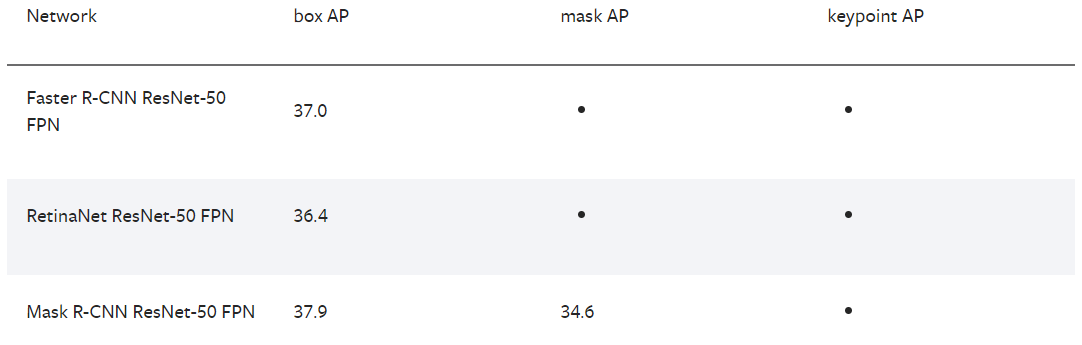
\includegraphics{image_report/porownanie.png} \newline
\textbf{Image 1} - Porównanie

\hypertarget{zbiory-danych}{%
\subsection{Zbiory danych:}\label{zbiory-danych}}

W celu porówniania działania obu serwisów sprawdziliśmy trzy zbiory
danych: 
\begin{itemize}
    \item Monkey, Cat and Dog detection (30 MB) -
\href{https://www.kaggle.com/tarunbisht11/yolo-animal-detection-small}{Kaggle},
    \item Fruit Images for Object Detection (28 MB) -
\href{https://www.kaggle.com/mbkinaci/fruit-images-for-object-detection?select=train_zip}{Kaggle}
\item Card detection (38,6 MB) -
\href{https://github.com/EdjeElectronics/TensorFlow-Object-Detection-API-Tutorial-Train-Multiple-Objects-Windows-10/tree/master/images}{Github}
\end{itemize}
Poniżej zostały dostarczone wytrenowane modeli na wyżej omówionych
zbiorach danych.

\hypertarget{azure-machine-learning-configuration}{%
\section{Azure Machine Learning
Configuration}\label{azure-machine-learning-configuration}}

Poniżej zostały dostarczone wytrenowane modeli na wyżej omówionych
zbiorach danych.

    Podłączanie bibliotek i pakietów:

    \begin{tcolorbox}[breakable, size=fbox, boxrule=1pt, pad at break*=1mm,colback=cellbackground, colframe=cellborder]
\prompt{In}{incolor}{1}{\boxspacing}
\begin{Verbatim}[commandchars=\\\{\}]
\PY{k+kn}{import} \PY{n+nn}{azureml}\PY{n+nn}{.}\PY{n+nn}{core}
\PY{k+kn}{from} \PY{n+nn}{azureml}\PY{n+nn}{.}\PY{n+nn}{core} \PY{k+kn}{import} \PY{n}{Workspace}
\PY{k+kn}{from} \PY{n+nn}{dotenv} \PY{k+kn}{import} \PY{n}{set\PYZus{}key}\PY{p}{,} \PY{n}{get\PYZus{}key}\PY{p}{,} \PY{n}{find\PYZus{}dotenv}
\PY{k+kn}{from} \PY{n+nn}{pathlib} \PY{k+kn}{import} \PY{n}{Path}
\PY{k+kn}{from} \PY{n+nn}{utilities} \PY{k+kn}{import} \PY{n}{get\PYZus{}auth}
\end{Verbatim}
\end{tcolorbox}

    Pokazanie poprawnego podłączenie do Workspace Azure. Wyświetlenie
wersji:

    \begin{tcolorbox}[breakable, size=fbox, boxrule=1pt, pad at break*=1mm,colback=cellbackground, colframe=cellborder]
\prompt{In}{incolor}{2}{\boxspacing}
\begin{Verbatim}[commandchars=\\\{\}]
\PY{n+nb}{print}\PY{p}{(}\PY{l+s+s2}{\PYZdq{}}\PY{l+s+s2}{You are currently using version}\PY{l+s+s2}{\PYZdq{}}\PY{p}{,} \PY{n}{azureml}\PY{o}{.}\PY{n}{core}\PY{o}{.}\PY{n}{VERSION}\PY{p}{,} \PY{l+s+s2}{\PYZdq{}}\PY{l+s+s2}{of the Azure ML SDK}\PY{l+s+s2}{\PYZdq{}}\PY{p}{)}
\end{Verbatim}
\end{tcolorbox}

    \begin{Verbatim}[commandchars=\\\{\}]
You are currently using version 1.17.0 of the Azure ML SDK
    \end{Verbatim}

    Konfiguracja Azure oraz environment

    \begin{tcolorbox}[breakable, size=fbox, boxrule=1pt, pad at break*=1mm,colback=cellbackground, colframe=cellborder]
\prompt{In}{incolor}{3}{\boxspacing}
\begin{Verbatim}[commandchars=\\\{\}]
\PY{k+kn}{import} \PY{n+nn}{os}
\PY{n}{subscription\PYZus{}id} \PY{o}{=} \PY{n}{os}\PY{o}{.}\PY{n}{environ}\PY{p}{[}\PY{l+s+s1}{\PYZsq{}}\PY{l+s+s1}{SUB\PYZus{}ID}\PY{l+s+s1}{\PYZsq{}}\PY{p}{]}
\PY{n}{resource\PYZus{}group} \PY{o}{=} \PY{l+s+s2}{\PYZdq{}}\PY{l+s+s2}{ProjektAzure}\PY{l+s+s2}{\PYZdq{}}
\PY{n}{workspace\PYZus{}name} \PY{o}{=} \PY{l+s+s2}{\PYZdq{}}\PY{l+s+s2}{ProjektAzure}\PY{l+s+s2}{\PYZdq{}}
\PY{n}{workspace\PYZus{}region} \PY{o}{=} \PY{l+s+s2}{\PYZdq{}}\PY{l+s+s2}{East US}\PY{l+s+s2}{\PYZdq{}}
\end{Verbatim}
\end{tcolorbox}

    Znajdowanie zasobu oraz podłączenie po przez kluczy oraz subskrypcje:

    \begin{tcolorbox}[breakable, size=fbox, boxrule=1pt, pad at break*=1mm,colback=cellbackground, colframe=cellborder]
\prompt{In}{incolor}{4}{\boxspacing}
\begin{Verbatim}[commandchars=\\\{\}]
\PY{n}{env\PYZus{}path} \PY{o}{=} \PY{n}{find\PYZus{}dotenv}\PY{p}{(}\PY{p}{)}
\PY{k}{if} \PY{n}{env\PYZus{}path} \PY{o}{==} \PY{l+s+s2}{\PYZdq{}}\PY{l+s+s2}{\PYZdq{}}\PY{p}{:}
    \PY{n}{Path}\PY{p}{(}\PY{l+s+s2}{\PYZdq{}}\PY{l+s+s2}{.env}\PY{l+s+s2}{\PYZdq{}}\PY{p}{)}\PY{o}{.}\PY{n}{touch}\PY{p}{(}\PY{p}{)}
    \PY{n}{env\PYZus{}path} \PY{o}{=} \PY{n}{find\PYZus{}dotenv}\PY{p}{(}\PY{p}{)}
\end{Verbatim}
\end{tcolorbox}

    \begin{tcolorbox}[breakable, size=fbox, boxrule=1pt, pad at break*=1mm,colback=cellbackground, colframe=cellborder]
\prompt{In}{incolor}{5}{\boxspacing}
\begin{Verbatim}[commandchars=\\\{\}]
\PY{n}{set\PYZus{}key}\PY{p}{(}\PY{n}{env\PYZus{}path}\PY{p}{,} \PY{l+s+s2}{\PYZdq{}}\PY{l+s+s2}{subscription\PYZus{}id}\PY{l+s+s2}{\PYZdq{}}\PY{p}{,} \PY{n}{subscription\PYZus{}id}\PY{p}{)} 
\PY{n}{set\PYZus{}key}\PY{p}{(}\PY{n}{env\PYZus{}path}\PY{p}{,} \PY{l+s+s2}{\PYZdq{}}\PY{l+s+s2}{resource\PYZus{}group}\PY{l+s+s2}{\PYZdq{}}\PY{p}{,} \PY{n}{resource\PYZus{}group}\PY{p}{)}
\PY{n}{set\PYZus{}key}\PY{p}{(}\PY{n}{env\PYZus{}path}\PY{p}{,} \PY{l+s+s2}{\PYZdq{}}\PY{l+s+s2}{workspace\PYZus{}name}\PY{l+s+s2}{\PYZdq{}}\PY{p}{,} \PY{n}{workspace\PYZus{}name}\PY{p}{)}
\PY{n}{set\PYZus{}key}\PY{p}{(}\PY{n}{env\PYZus{}path}\PY{p}{,} \PY{l+s+s2}{\PYZdq{}}\PY{l+s+s2}{workspace\PYZus{}region}\PY{l+s+s2}{\PYZdq{}}\PY{p}{,} \PY{n}{workspace\PYZus{}region}\PY{p}{)}
\end{Verbatim}
\end{tcolorbox}

            \begin{tcolorbox}[breakable, size=fbox, boxrule=.5pt, pad at break*=1mm, opacityfill=0]
\prompt{Out}{outcolor}{5}{\boxspacing}
\begin{Verbatim}[commandchars=\\\{\}]
(True, 'workspace\_region', 'East US')
\end{Verbatim}
\end{tcolorbox}
        
    Stworzenie roboczego obszaru przy użyciu określonych parametrów i
zapisanie szczegółów obszaru roboczego do pliku konfiguracyjnego:

    \begin{tcolorbox}[breakable, size=fbox, boxrule=1pt, pad at break*=1mm,colback=cellbackground, colframe=cellborder]
\prompt{In}{incolor}{6}{\boxspacing}
\begin{Verbatim}[commandchars=\\\{\}]
\PY{c+c1}{\PYZsh{} Create the workspace using the specified parameters}
\PY{n}{ws} \PY{o}{=} \PY{n}{Workspace}\PY{o}{.}\PY{n}{create}\PY{p}{(}
    \PY{n}{name}\PY{o}{=}\PY{n}{workspace\PYZus{}name}\PY{p}{,}
    \PY{n}{subscription\PYZus{}id}\PY{o}{=}\PY{n}{subscription\PYZus{}id}\PY{p}{,}
    \PY{n}{resource\PYZus{}group}\PY{o}{=}\PY{n}{resource\PYZus{}group}\PY{p}{,}
    \PY{n}{location}\PY{o}{=}\PY{n}{workspace\PYZus{}region}\PY{p}{,}
    \PY{n}{create\PYZus{}resource\PYZus{}group}\PY{o}{=}\PY{k+kc}{True}\PY{p}{,}
    \PY{n}{auth}\PY{o}{=}\PY{n}{get\PYZus{}auth}\PY{p}{(}\PY{n}{env\PYZus{}path}\PY{p}{)}\PY{p}{,}
    \PY{n}{exist\PYZus{}ok}\PY{o}{=}\PY{k+kc}{True}\PY{p}{,}
\PY{p}{)}

\PY{c+c1}{\PYZsh{} write the details of the workspace to a configuration file}
\PY{n}{ws}\PY{o}{.}\PY{n}{write\PYZus{}config}\PY{p}{(}\PY{p}{)}
\end{Verbatim}
\end{tcolorbox}

    Poniżej można zobaczyć informację dotyczące roboczego obszru (jeżeli
odkomentować ws.get\_details)

    \begin{tcolorbox}[breakable, size=fbox, boxrule=1pt, pad at break*=1mm,colback=cellbackground, colframe=cellborder]
\prompt{In}{incolor}{8}{\boxspacing}
\begin{Verbatim}[commandchars=\\\{\}]
\PY{c+c1}{\PYZsh{} load workspace configuration}
\PY{n}{ws} \PY{o}{=} \PY{n}{Workspace}\PY{o}{.}\PY{n}{from\PYZus{}config}\PY{p}{(}\PY{n}{auth}\PY{o}{=}\PY{n}{get\PYZus{}auth}\PY{p}{(}\PY{n}{env\PYZus{}path}\PY{p}{)}\PY{p}{)}
\PY{c+c1}{\PYZsh{}ws.get\PYZus{}details()}
\end{Verbatim}
\end{tcolorbox}

    Poniżej jest importowanie bibliotek oraz podłączenie ścieżki do plików,
które wskazują na moduły:

    \begin{tcolorbox}[breakable, size=fbox, boxrule=1pt, pad at break*=1mm,colback=cellbackground, colframe=cellborder]
\prompt{In}{incolor}{9}{\boxspacing}
\begin{Verbatim}[commandchars=\\\{\}]
\PY{k+kn}{import} \PY{n+nn}{sys}

\PY{n}{sys}\PY{o}{.}\PY{n}{path}\PY{o}{.}\PY{n}{append}\PY{p}{(}\PY{l+s+s2}{\PYZdq{}}\PY{l+s+s2}{scripts}\PY{l+s+s2}{\PYZdq{}}\PY{p}{)}
\PY{n}{sys}\PY{o}{.}\PY{n}{path}\PY{o}{.}\PY{n}{append}\PY{p}{(}\PY{l+s+s2}{\PYZdq{}}\PY{l+s+s2}{scripts/cocoapi/PythonAPI/}\PY{l+s+s2}{\PYZdq{}}\PY{p}{)}

\PY{k+kn}{import} \PY{n+nn}{azureml}\PY{n+nn}{.}\PY{n+nn}{core}
\PY{k+kn}{from} \PY{n+nn}{azureml}\PY{n+nn}{.}\PY{n+nn}{core} \PY{k+kn}{import} \PY{n}{Workspace}\PY{p}{,} \PY{n}{Experiment}
\PY{k+kn}{from} \PY{n+nn}{azureml}\PY{n+nn}{.}\PY{n+nn}{widgets} \PY{k+kn}{import} \PY{n}{RunDetails}
\PY{k+kn}{from} \PY{n+nn}{azureml}\PY{n+nn}{.}\PY{n+nn}{train}\PY{n+nn}{.}\PY{n+nn}{dnn} \PY{k+kn}{import} \PY{n}{PyTorch}

\PY{k+kn}{from} \PY{n+nn}{dotenv} \PY{k+kn}{import} \PY{n}{set\PYZus{}key}\PY{p}{,} \PY{n}{get\PYZus{}key}\PY{p}{,} \PY{n}{find\PYZus{}dotenv}
\PY{k+kn}{from} \PY{n+nn}{utilities} \PY{k+kn}{import} \PY{n}{get\PYZus{}auth}\PY{p}{,} \PY{n}{download\PYZus{}data}

\PY{k+kn}{import} \PY{n+nn}{torch}
\PY{k+kn}{from} \PY{n+nn}{scripts}\PY{n+nn}{.}\PY{n+nn}{XMLDataset} \PY{k+kn}{import} \PY{n}{BuildDataset}\PY{p}{,} \PY{n}{get\PYZus{}transform}
\PY{k+kn}{from} \PY{n+nn}{scripts}\PY{n+nn}{.}\PY{n+nn}{maskrcnn\PYZus{}model} \PY{k+kn}{import} \PY{n}{get\PYZus{}model}

\PY{k+kn}{from} \PY{n+nn}{PIL} \PY{k+kn}{import} \PY{n}{Image}\PY{p}{,} \PY{n}{ImageDraw}
\PY{k+kn}{from} \PY{n+nn}{IPython}\PY{n+nn}{.}\PY{n+nn}{display} \PY{k+kn}{import} \PY{n}{display}

\PY{c+c1}{\PYZsh{} check core SDK version number}
\PY{n+nb}{print}\PY{p}{(}\PY{l+s+s2}{\PYZdq{}}\PY{l+s+s2}{Azure ML SDK Version: }\PY{l+s+s2}{\PYZdq{}}\PY{p}{,} \PY{n}{azureml}\PY{o}{.}\PY{n}{core}\PY{o}{.}\PY{n}{VERSION}\PY{p}{)}
\end{Verbatim}
\end{tcolorbox}

    \begin{Verbatim}[commandchars=\\\{\}]
Azure ML SDK Version:  1.17.0
    \end{Verbatim}

    \hypertarget{implementacja-mask-r-cnn-model}{%
\subsection{Implementacja Mask R-CNN
model}\label{implementacja-mask-r-cnn-model}}

    \begin{tcolorbox}[breakable, size=fbox, boxrule=1pt, pad at break*=1mm,colback=cellbackground, colframe=cellborder]
\prompt{In}{incolor}{ }{\boxspacing}
\begin{Verbatim}[commandchars=\\\{\}]
\PY{c+c1}{\PYZsh{}UWAGA!UWAGA!UWAGA!}
\end{Verbatim}
\end{tcolorbox}

    \begin{tcolorbox}[breakable, size=fbox, boxrule=1pt, pad at break*=1mm,colback=cellbackground, colframe=cellborder]
\prompt{In}{incolor}{9}{\boxspacing}
\begin{Verbatim}[commandchars=\\\{\}]
\PY{o}{\PYZpc{}\PYZpc{}writefile} scripts/XMLDataset.py
\PY{k+kn}{import} \PY{n+nn}{os}
\PY{k+kn}{import} \PY{n+nn}{xml}\PY{n+nn}{.}\PY{n+nn}{etree}\PY{n+nn}{.}\PY{n+nn}{ElementTree} \PY{k}{as} \PY{n+nn}{ET}
\PY{k+kn}{import} \PY{n+nn}{torch}
\PY{k+kn}{import} \PY{n+nn}{transforms} \PY{k}{as} \PY{n+nn}{T}
\PY{k+kn}{from} \PY{n+nn}{PIL} \PY{k+kn}{import} \PY{n}{Image}


\PY{k}{class} \PY{n+nc}{BuildDataset}\PY{p}{(}\PY{n}{torch}\PY{o}{.}\PY{n}{utils}\PY{o}{.}\PY{n}{data}\PY{o}{.}\PY{n}{Dataset}\PY{p}{)}\PY{p}{:}
    \PY{k}{def} \PY{n+nf+fm}{\PYZus{}\PYZus{}init\PYZus{}\PYZus{}}\PY{p}{(}\PY{n+nb+bp}{self}\PY{p}{,} \PY{n}{root}\PY{p}{,}\PY{n}{dataset}\PY{p}{,} \PY{n}{transforms}\PY{o}{=}\PY{k+kc}{None}\PY{p}{,} \PY{n}{train}\PY{o}{=}\PY{k+kc}{True}\PY{p}{)}\PY{p}{:}
        \PY{n+nb+bp}{self}\PY{o}{.}\PY{n}{root} \PY{o}{=} \PY{n}{root}
        \PY{n+nb+bp}{self}\PY{o}{.}\PY{n}{transforms} \PY{o}{=} \PY{n}{transforms}
        \PY{c+c1}{\PYZsh{}self.labels\PYZus{}dict = \PYZob{}\PYZsq{}obama\PYZsq{}: 1\PYZcb{}}
        \PY{c+c1}{\PYZsh{}self.labels\PYZus{}dict = \PYZob{}\PYZsq{}ace\PYZsq{}: 1, \PYZsq{}king\PYZsq{}: 2, \PYZsq{}queen\PYZsq{}: 3, \PYZsq{}jack\PYZsq{}: 4, \PYZsq{}ten\PYZsq{}: 5, \PYZsq{}nine\PYZsq{}: 6\PYZcb{}}

\PY{c+c1}{\PYZsh{}        self.labels\PYZus{}dict = \PYZob{}\PYZsq{}cat\PYZsq{}: 1, \PYZsq{}dog\PYZsq{}: 2, \PYZsq{}monkey\PYZsq{}: 3\PYZcb{}}
\PY{c+c1}{\PYZsh{}         self.labels\PYZus{}dict[\PYZsq{}cat\PYZsq{}] = 1}
\PY{c+c1}{\PYZsh{}         self.labels\PYZus{}dict[\PYZsq{}dog\PYZsq{}] = 2}
\PY{c+c1}{\PYZsh{}         self.labels\PYZus{}dict[\PYZsq{}monkey\PYZsq{}] = 3}
        \PY{c+c1}{\PYZsh{} load all image files}
        \PY{k}{if} \PY{n}{dataset}  \PY{o}{==} \PY{l+s+s2}{\PYZdq{}}\PY{l+s+s2}{Fruit}\PY{l+s+s2}{\PYZdq{}}\PY{p}{:}
            \PY{n+nb+bp}{self}\PY{o}{.}\PY{n}{labels\PYZus{}dict} \PY{o}{=} \PY{p}{\PYZob{}}\PY{l+s+s1}{\PYZsq{}}\PY{l+s+s1}{apple}\PY{l+s+s1}{\PYZsq{}}\PY{p}{:} \PY{l+m+mi}{1}\PY{p}{,} \PY{l+s+s1}{\PYZsq{}}\PY{l+s+s1}{orange}\PY{l+s+s1}{\PYZsq{}}\PY{p}{:} \PY{l+m+mi}{2}\PY{p}{,} \PY{l+s+s1}{\PYZsq{}}\PY{l+s+s1}{banana}\PY{l+s+s1}{\PYZsq{}}\PY{p}{:} \PY{l+m+mi}{3}\PY{p}{\PYZcb{}}
        \PY{k}{elif} \PY{n}{dataset} \PY{o}{==} \PY{l+s+s2}{\PYZdq{}}\PY{l+s+s2}{PlayCards}\PY{l+s+s2}{\PYZdq{}}\PY{p}{:}
            \PY{n+nb+bp}{self}\PY{o}{.}\PY{n}{labels\PYZus{}dict} \PY{o}{=} \PY{p}{\PYZob{}}\PY{l+s+s1}{\PYZsq{}}\PY{l+s+s1}{ace}\PY{l+s+s1}{\PYZsq{}}\PY{p}{:} \PY{l+m+mi}{1}\PY{p}{,} \PY{l+s+s1}{\PYZsq{}}\PY{l+s+s1}{king}\PY{l+s+s1}{\PYZsq{}}\PY{p}{:} \PY{l+m+mi}{2}\PY{p}{,} \PY{l+s+s1}{\PYZsq{}}\PY{l+s+s1}{queen}\PY{l+s+s1}{\PYZsq{}}\PY{p}{:} \PY{l+m+mi}{3}\PY{p}{,} \PY{l+s+s1}{\PYZsq{}}\PY{l+s+s1}{jack}\PY{l+s+s1}{\PYZsq{}}\PY{p}{:} \PY{l+m+mi}{4}\PY{p}{,} \PY{l+s+s1}{\PYZsq{}}\PY{l+s+s1}{ten}\PY{l+s+s1}{\PYZsq{}}\PY{p}{:} \PY{l+m+mi}{5}\PY{p}{,} \PY{l+s+s1}{\PYZsq{}}\PY{l+s+s1}{nine}\PY{l+s+s1}{\PYZsq{}}\PY{p}{:} \PY{l+m+mi}{6}\PY{p}{\PYZcb{}}
        \PY{k}{else}\PY{p}{:}
            \PY{n+nb+bp}{self}\PY{o}{.}\PY{n}{labels\PYZus{}dict} \PY{o}{=} \PY{p}{\PYZob{}}\PY{l+s+s1}{\PYZsq{}}\PY{l+s+s1}{cat}\PY{l+s+s1}{\PYZsq{}}\PY{p}{:} \PY{l+m+mi}{1}\PY{p}{,} \PY{l+s+s1}{\PYZsq{}}\PY{l+s+s1}{dog}\PY{l+s+s1}{\PYZsq{}}\PY{p}{:} \PY{l+m+mi}{2}\PY{p}{,} \PY{l+s+s1}{\PYZsq{}}\PY{l+s+s1}{monkey}\PY{l+s+s1}{\PYZsq{}}\PY{p}{:} \PY{l+m+mi}{3}\PY{p}{\PYZcb{}}
        \PY{k}{if} \PY{n}{train}\PY{p}{:}
            \PY{n+nb}{print}\PY{p}{(}\PY{l+s+sa}{f}\PY{l+s+s2}{\PYZdq{}}\PY{l+s+s2}{Data/}\PY{l+s+si}{\PYZob{}}\PY{n}{dataset}\PY{l+s+si}{\PYZcb{}}\PY{l+s+s2}{/JPEGImages}\PY{l+s+s2}{\PYZdq{}}\PY{p}{)}
            \PY{n+nb}{print}\PY{p}{(}\PY{l+s+s2}{\PYZdq{}}\PY{l+s+s2}{Data/}\PY{l+s+s2}{\PYZdq{}}\PY{o}{+}\PY{n}{dataset}\PY{o}{+}\PY{l+s+s2}{\PYZdq{}}\PY{l+s+s2}{/JPEGImages}\PY{l+s+s2}{\PYZdq{}}\PY{p}{)}
            \PY{n+nb+bp}{self}\PY{o}{.}\PY{n}{imgs\PYZus{}path} \PY{o}{=} \PY{n}{os}\PY{o}{.}\PY{n}{path}\PY{o}{.}\PY{n}{join}\PY{p}{(}\PY{n}{root}\PY{p}{,} \PY{l+s+sa}{f}\PY{l+s+s2}{\PYZdq{}}\PY{l+s+s2}{Data/}\PY{l+s+si}{\PYZob{}}\PY{n}{dataset}\PY{l+s+si}{\PYZcb{}}\PY{l+s+s2}{/JPEGImages}\PY{l+s+s2}{\PYZdq{}}\PY{p}{)}
            \PY{n+nb}{print}\PY{p}{(}\PY{n+nb}{type}\PY{p}{(}\PY{n}{dataset}\PY{p}{)}\PY{p}{)}
            \PY{n+nb+bp}{self}\PY{o}{.}\PY{n}{imgs} \PY{o}{=} \PY{n+nb}{list}\PY{p}{(}\PY{n+nb}{sorted}\PY{p}{(}\PY{n}{os}\PY{o}{.}\PY{n}{listdir}\PY{p}{(}\PY{n+nb+bp}{self}\PY{o}{.}\PY{n}{imgs\PYZus{}path}\PY{p}{)}\PY{p}{)}\PY{p}{)}
            \PY{n+nb+bp}{self}\PY{o}{.}\PY{n}{xmls\PYZus{}path} \PY{o}{=} \PY{n}{os}\PY{o}{.}\PY{n}{path}\PY{o}{.}\PY{n}{join}\PY{p}{(}\PY{n}{root}\PY{p}{,} \PY{l+s+sa}{f}\PY{l+s+s2}{\PYZdq{}}\PY{l+s+s2}{Data/}\PY{l+s+si}{\PYZob{}}\PY{n}{dataset}\PY{l+s+si}{\PYZcb{}}\PY{l+s+s2}{/Annotations}\PY{l+s+s2}{\PYZdq{}}\PY{p}{)}
        \PY{k}{else}\PY{p}{:}
            \PY{n+nb+bp}{self}\PY{o}{.}\PY{n}{imgs\PYZus{}path} \PY{o}{=} \PY{n}{os}\PY{o}{.}\PY{n}{path}\PY{o}{.}\PY{n}{join}\PY{p}{(}\PY{n}{root}\PY{p}{,} \PY{l+s+sa}{f}\PY{l+s+s2}{\PYZdq{}}\PY{l+s+s2}{Data/}\PY{l+s+si}{\PYZob{}}\PY{n}{dataset}\PY{l+s+si}{\PYZcb{}}\PY{l+s+s2}{/JPEGImagesTest}\PY{l+s+s2}{\PYZdq{}}\PY{p}{)}
            \PY{n+nb+bp}{self}\PY{o}{.}\PY{n}{imgs} \PY{o}{=} \PY{n+nb}{list}\PY{p}{(}\PY{n+nb}{sorted}\PY{p}{(}\PY{n}{os}\PY{o}{.}\PY{n}{listdir}\PY{p}{(}\PY{n+nb+bp}{self}\PY{o}{.}\PY{n}{imgs\PYZus{}path}\PY{p}{)}\PY{p}{)}\PY{p}{)}
            \PY{n+nb+bp}{self}\PY{o}{.}\PY{n}{xmls\PYZus{}path} \PY{o}{=} \PY{n}{os}\PY{o}{.}\PY{n}{path}\PY{o}{.}\PY{n}{join}\PY{p}{(}\PY{n}{root}\PY{p}{,} \PY{l+s+sa}{f}\PY{l+s+s2}{\PYZdq{}}\PY{l+s+s2}{Data/}\PY{l+s+si}{\PYZob{}}\PY{n}{dataset}\PY{l+s+si}{\PYZcb{}}\PY{l+s+s2}{/AnnotationsTest}\PY{l+s+s2}{\PYZdq{}}\PY{p}{)}
    
\PY{c+c1}{\PYZsh{}         if train:}
\PY{c+c1}{\PYZsh{}             self.imgs\PYZus{}path = os.path.join(root, \PYZdq{}Data/PlayCards/JPEGImages\PYZdq{})}
\PY{c+c1}{\PYZsh{}             self.imgs = list(sorted(os.listdir(self.imgs\PYZus{}path)))}
\PY{c+c1}{\PYZsh{}             self.xmls\PYZus{}path = os.path.join(root, \PYZdq{}Data/PlayCards/Annotations\PYZdq{})}
\PY{c+c1}{\PYZsh{}         else:}
\PY{c+c1}{\PYZsh{}             self.imgs\PYZus{}path = os.path.join(root, \PYZdq{}Data/PlayCards/JPEGImagesTest\PYZdq{})}
\PY{c+c1}{\PYZsh{}             self.imgs = list(sorted(os.listdir(self.imgs\PYZus{}path)))}
\PY{c+c1}{\PYZsh{}             self.xmls\PYZus{}path = os.path.join(root, \PYZdq{}Data/PlayCards/AnnotationsTest\PYZdq{})}
\PY{c+c1}{\PYZsh{}         if train:}
\PY{c+c1}{\PYZsh{}             self.imgs\PYZus{}path = os.path.join(root, \PYZdq{}Data/monkeyCats/JPEGImages\PYZdq{})}
\PY{c+c1}{\PYZsh{}             self.imgs = list(sorted(os.listdir(self.imgs\PYZus{}path)))}
\PY{c+c1}{\PYZsh{}             self.xmls\PYZus{}path = os.path.join(root, \PYZdq{}Data/monkeyCats/Annotations\PYZdq{})}
\PY{c+c1}{\PYZsh{}         else:}
\PY{c+c1}{\PYZsh{}             self.imgs\PYZus{}path = os.path.join(root, \PYZdq{}Data/monkeyCats/JPEGImagesTest\PYZdq{})}
\PY{c+c1}{\PYZsh{}             self.imgs = list(sorted(os.listdir(self.imgs\PYZus{}path)))}
\PY{c+c1}{\PYZsh{}             self.xmls\PYZus{}path = os.path.join(root, \PYZdq{}Data/monkeyCats/AnnotationsTest\PYZdq{})}

    \PY{k}{def} \PY{n+nf+fm}{\PYZus{}\PYZus{}getitem\PYZus{}\PYZus{}}\PY{p}{(}\PY{n+nb+bp}{self}\PY{p}{,} \PY{n}{idx}\PY{p}{)}\PY{p}{:}
        \PY{n}{img\PYZus{}path} \PY{o}{=} \PY{n}{os}\PY{o}{.}\PY{n}{path}\PY{o}{.}\PY{n}{join}\PY{p}{(}\PY{n+nb+bp}{self}\PY{o}{.}\PY{n}{imgs\PYZus{}path}\PY{p}{,} \PY{n+nb+bp}{self}\PY{o}{.}\PY{n}{imgs}\PY{p}{[}\PY{n}{idx}\PY{p}{]}\PY{p}{)}
        \PY{n}{xml\PYZus{}path} \PY{o}{=} \PY{n}{os}\PY{o}{.}\PY{n}{path}\PY{o}{.}\PY{n}{join}\PY{p}{(}
            \PY{n+nb+bp}{self}\PY{o}{.}\PY{n}{xmls\PYZus{}path}\PY{p}{,} \PY{l+s+s2}{\PYZdq{}}\PY{l+s+si}{\PYZob{}\PYZcb{}}\PY{l+s+s2}{.xml}\PY{l+s+s2}{\PYZdq{}}\PY{o}{.}\PY{n}{format}\PY{p}{(}\PY{n+nb+bp}{self}\PY{o}{.}\PY{n}{imgs}\PY{p}{[}\PY{n}{idx}\PY{p}{]}\PY{o}{.}\PY{n}{strip}\PY{p}{(}\PY{l+s+s2}{\PYZdq{}}\PY{l+s+s2}{.jpg}\PY{l+s+s2}{\PYZdq{}}\PY{p}{)}\PY{p}{)}
        \PY{p}{)}
        \PY{n}{img} \PY{o}{=} \PY{n}{Image}\PY{o}{.}\PY{n}{open}\PY{p}{(}\PY{n}{img\PYZus{}path}\PY{p}{)}\PY{o}{.}\PY{n}{convert}\PY{p}{(}\PY{l+s+s2}{\PYZdq{}}\PY{l+s+s2}{RGB}\PY{l+s+s2}{\PYZdq{}}\PY{p}{)}

        \PY{c+c1}{\PYZsh{} parse XML annotation}
        \PY{n}{tree} \PY{o}{=} \PY{n}{ET}\PY{o}{.}\PY{n}{parse}\PY{p}{(}\PY{n}{xml\PYZus{}path}\PY{p}{)}
        \PY{n}{t\PYZus{}root} \PY{o}{=} \PY{n}{tree}\PY{o}{.}\PY{n}{getroot}\PY{p}{(}\PY{p}{)}

        \PY{c+c1}{\PYZsh{} get bounding box coordinates}
        \PY{n}{boxes} \PY{o}{=} \PY{p}{[}\PY{p}{]}
        \PY{n}{labels} \PY{o}{=} \PY{p}{[}\PY{p}{]}
        \PY{k}{for} \PY{n}{obj} \PY{o+ow}{in} \PY{n}{t\PYZus{}root}\PY{o}{.}\PY{n}{findall}\PY{p}{(}\PY{l+s+s2}{\PYZdq{}}\PY{l+s+s2}{object}\PY{l+s+s2}{\PYZdq{}}\PY{p}{)}\PY{p}{:}
            \PY{n}{bnd\PYZus{}box} \PY{o}{=} \PY{n}{obj}\PY{o}{.}\PY{n}{find}\PY{p}{(}\PY{l+s+s2}{\PYZdq{}}\PY{l+s+s2}{bndbox}\PY{l+s+s2}{\PYZdq{}}\PY{p}{)}
            \PY{n}{xmin} \PY{o}{=} \PY{n+nb}{float}\PY{p}{(}\PY{n}{bnd\PYZus{}box}\PY{o}{.}\PY{n}{find}\PY{p}{(}\PY{l+s+s2}{\PYZdq{}}\PY{l+s+s2}{xmin}\PY{l+s+s2}{\PYZdq{}}\PY{p}{)}\PY{o}{.}\PY{n}{text}\PY{p}{)}
            \PY{n}{xmax} \PY{o}{=} \PY{n+nb}{float}\PY{p}{(}\PY{n}{bnd\PYZus{}box}\PY{o}{.}\PY{n}{find}\PY{p}{(}\PY{l+s+s2}{\PYZdq{}}\PY{l+s+s2}{xmax}\PY{l+s+s2}{\PYZdq{}}\PY{p}{)}\PY{o}{.}\PY{n}{text}\PY{p}{)}
            \PY{n}{ymin} \PY{o}{=} \PY{n+nb}{float}\PY{p}{(}\PY{n}{bnd\PYZus{}box}\PY{o}{.}\PY{n}{find}\PY{p}{(}\PY{l+s+s2}{\PYZdq{}}\PY{l+s+s2}{ymin}\PY{l+s+s2}{\PYZdq{}}\PY{p}{)}\PY{o}{.}\PY{n}{text}\PY{p}{)}
            \PY{n}{ymax} \PY{o}{=} \PY{n+nb}{float}\PY{p}{(}\PY{n}{bnd\PYZus{}box}\PY{o}{.}\PY{n}{find}\PY{p}{(}\PY{l+s+s2}{\PYZdq{}}\PY{l+s+s2}{ymax}\PY{l+s+s2}{\PYZdq{}}\PY{p}{)}\PY{o}{.}\PY{n}{text}\PY{p}{)}
            \PY{n}{boxes}\PY{o}{.}\PY{n}{append}\PY{p}{(}\PY{p}{[}\PY{n}{xmin}\PY{p}{,} \PY{n}{ymin}\PY{p}{,} \PY{n}{xmax}\PY{p}{,} \PY{n}{ymax}\PY{p}{]}\PY{p}{)}
            \PY{n}{label\PYZus{}name} \PY{o}{=} \PY{n+nb}{str}\PY{p}{(}\PY{n}{obj}\PY{o}{.}\PY{n}{find}\PY{p}{(}\PY{l+s+s2}{\PYZdq{}}\PY{l+s+s2}{name}\PY{l+s+s2}{\PYZdq{}}\PY{p}{)}\PY{o}{.}\PY{n}{text}\PY{p}{)}
\PY{c+c1}{\PYZsh{}             if self.labels\PYZus{}dict:}
\PY{c+c1}{\PYZsh{}                 if label\PYZus{}name not in self.labels\PYZus{}dict.keys():}
\PY{c+c1}{\PYZsh{}                     self.labels\PYZus{}dict[label\PYZus{}name] = max(self.labels\PYZus{}dict.values()) + 1}
\PY{c+c1}{\PYZsh{}             else:}
\PY{c+c1}{\PYZsh{}                 self.labels\PYZus{}dict[label\PYZus{}name] = 1}
\PY{c+c1}{\PYZsh{}             print(label\PYZus{}name + \PYZdq{}: \PYZdq{} + str(self.labels\PYZus{}dict[label\PYZus{}name]))}
            \PY{n}{labels}\PY{o}{.}\PY{n}{append}\PY{p}{(}\PY{n+nb+bp}{self}\PY{o}{.}\PY{n}{labels\PYZus{}dict}\PY{p}{[}\PY{n}{label\PYZus{}name}\PY{p}{]}\PY{p}{)}
        \PY{n}{num\PYZus{}objs} \PY{o}{=} \PY{n+nb}{len}\PY{p}{(}\PY{n}{boxes}\PY{p}{)}
        \PY{n}{boxes} \PY{o}{=} \PY{n}{torch}\PY{o}{.}\PY{n}{as\PYZus{}tensor}\PY{p}{(}\PY{n}{boxes}\PY{p}{,} \PY{n}{dtype}\PY{o}{=}\PY{n}{torch}\PY{o}{.}\PY{n}{float32}\PY{p}{)}

        \PY{c+c1}{\PYZsh{} there is only one class}
        \PY{n}{labels} \PY{o}{=} \PY{n}{torch}\PY{o}{.}\PY{n}{as\PYZus{}tensor}\PY{p}{(}\PY{n}{labels}\PY{p}{)}
\PY{c+c1}{\PYZsh{}         print(labels)}
\PY{c+c1}{\PYZsh{}         labels = torch.ones((num\PYZus{}objs,), dtype=torch.int64)}
        \PY{n}{image\PYZus{}id} \PY{o}{=} \PY{n}{torch}\PY{o}{.}\PY{n}{tensor}\PY{p}{(}\PY{p}{[}\PY{n}{idx}\PY{p}{]}\PY{p}{)}

        \PY{c+c1}{\PYZsh{} area of the bounding box, used during evaluation with the COCO metric for small, medium and large boxes}
        \PY{n}{area} \PY{o}{=} \PY{p}{(}\PY{n}{boxes}\PY{p}{[}\PY{p}{:}\PY{p}{,} \PY{l+m+mi}{3}\PY{p}{]} \PY{o}{\PYZhy{}} \PY{n}{boxes}\PY{p}{[}\PY{p}{:}\PY{p}{,} \PY{l+m+mi}{1}\PY{p}{]}\PY{p}{)} \PY{o}{*} \PY{p}{(}\PY{n}{boxes}\PY{p}{[}\PY{p}{:}\PY{p}{,} \PY{l+m+mi}{2}\PY{p}{]} \PY{o}{\PYZhy{}} \PY{n}{boxes}\PY{p}{[}\PY{p}{:}\PY{p}{,} \PY{l+m+mi}{0}\PY{p}{]}\PY{p}{)}

        \PY{c+c1}{\PYZsh{} suppose all instances are not crowd}
        \PY{n}{iscrowd} \PY{o}{=} \PY{n}{torch}\PY{o}{.}\PY{n}{zeros}\PY{p}{(}\PY{p}{(}\PY{n}{num\PYZus{}objs}\PY{p}{,}\PY{p}{)}\PY{p}{,} \PY{n}{dtype}\PY{o}{=}\PY{n}{torch}\PY{o}{.}\PY{n}{int64}\PY{p}{)}

        \PY{n}{target} \PY{o}{=} \PY{p}{\PYZob{}}\PY{p}{\PYZcb{}}
        \PY{n}{target}\PY{p}{[}\PY{l+s+s2}{\PYZdq{}}\PY{l+s+s2}{boxes}\PY{l+s+s2}{\PYZdq{}}\PY{p}{]} \PY{o}{=} \PY{n}{boxes}
        \PY{n}{target}\PY{p}{[}\PY{l+s+s2}{\PYZdq{}}\PY{l+s+s2}{labels}\PY{l+s+s2}{\PYZdq{}}\PY{p}{]} \PY{o}{=} \PY{n}{labels}
        \PY{n}{target}\PY{p}{[}\PY{l+s+s2}{\PYZdq{}}\PY{l+s+s2}{image\PYZus{}id}\PY{l+s+s2}{\PYZdq{}}\PY{p}{]} \PY{o}{=} \PY{n}{image\PYZus{}id}
        \PY{n}{target}\PY{p}{[}\PY{l+s+s2}{\PYZdq{}}\PY{l+s+s2}{area}\PY{l+s+s2}{\PYZdq{}}\PY{p}{]} \PY{o}{=} \PY{n}{area}
        \PY{n}{target}\PY{p}{[}\PY{l+s+s2}{\PYZdq{}}\PY{l+s+s2}{iscrowd}\PY{l+s+s2}{\PYZdq{}}\PY{p}{]} \PY{o}{=} \PY{n}{iscrowd}

        \PY{k}{if} \PY{n+nb+bp}{self}\PY{o}{.}\PY{n}{transforms} \PY{o+ow}{is} \PY{o+ow}{not} \PY{k+kc}{None}\PY{p}{:}
            \PY{n}{img}\PY{p}{,} \PY{n}{target} \PY{o}{=} \PY{n+nb+bp}{self}\PY{o}{.}\PY{n}{transforms}\PY{p}{(}\PY{n}{img}\PY{p}{,} \PY{n}{target}\PY{p}{)}

        \PY{k}{return} \PY{n}{img}\PY{p}{,} \PY{n}{target}

    \PY{k}{def} \PY{n+nf+fm}{\PYZus{}\PYZus{}len\PYZus{}\PYZus{}}\PY{p}{(}\PY{n+nb+bp}{self}\PY{p}{)}\PY{p}{:}
        \PY{k}{return} \PY{n+nb}{len}\PY{p}{(}\PY{n+nb+bp}{self}\PY{o}{.}\PY{n}{imgs}\PY{p}{)}


\PY{k}{def} \PY{n+nf}{get\PYZus{}transform}\PY{p}{(}\PY{n}{train}\PY{p}{)}\PY{p}{:}
    \PY{n}{transforms} \PY{o}{=} \PY{p}{[}\PY{p}{]}
    \PY{n}{transforms}\PY{o}{.}\PY{n}{append}\PY{p}{(}\PY{n}{T}\PY{o}{.}\PY{n}{ToTensor}\PY{p}{(}\PY{p}{)}\PY{p}{)}
    \PY{k}{if} \PY{n}{train}\PY{p}{:}
        \PY{n}{transforms}\PY{o}{.}\PY{n}{append}\PY{p}{(}\PY{n}{T}\PY{o}{.}\PY{n}{RandomHorizontalFlip}\PY{p}{(}\PY{l+m+mf}{0.5}\PY{p}{)}\PY{p}{)}
    \PY{k}{return} \PY{n}{T}\PY{o}{.}\PY{n}{Compose}\PY{p}{(}\PY{n}{transforms}\PY{p}{)}
\end{Verbatim}
\end{tcolorbox}

    \begin{Verbatim}[commandchars=\\\{\}]
Overwriting scripts/XMLDataset.py
    \end{Verbatim}

    \begin{tcolorbox}[breakable, size=fbox, boxrule=1pt, pad at break*=1mm,colback=cellbackground, colframe=cellborder]
\prompt{In}{incolor}{10}{\boxspacing}
\begin{Verbatim}[commandchars=\\\{\}]
\PY{o}{\PYZpc{}\PYZpc{}writefile} scripts/maskrcnn\PYZus{}model.py
\PY{k+kn}{import} \PY{n+nn}{torchvision}
\PY{k+kn}{from} \PY{n+nn}{torchvision}\PY{n+nn}{.}\PY{n+nn}{models}\PY{n+nn}{.}\PY{n+nn}{detection}\PY{n+nn}{.}\PY{n+nn}{faster\PYZus{}rcnn} \PY{k+kn}{import} \PY{n}{FastRCNNPredictor}
\PY{k+kn}{from} \PY{n+nn}{torchvision}\PY{n+nn}{.}\PY{n+nn}{models}\PY{n+nn}{.}\PY{n+nn}{detection}\PY{n+nn}{.}\PY{n+nn}{rpn} \PY{k+kn}{import} \PY{n}{AnchorGenerator}
\PY{k+kn}{from} \PY{n+nn}{torchvision}\PY{n+nn}{.}\PY{n+nn}{models}\PY{n+nn}{.}\PY{n+nn}{detection}\PY{n+nn}{.}\PY{n+nn}{rpn} \PY{k+kn}{import} \PY{n}{RPNHead}


\PY{k}{def} \PY{n+nf}{get\PYZus{}model}\PY{p}{(}
    \PY{n}{num\PYZus{}classes}\PY{p}{,}
    \PY{n}{anchor\PYZus{}sizes}\PY{p}{,}
    \PY{n}{anchor\PYZus{}aspect\PYZus{}ratios}\PY{p}{,}
    \PY{n}{rpn\PYZus{}nms\PYZus{}threshold}\PY{p}{,}
    \PY{n}{box\PYZus{}nms\PYZus{}threshold}\PY{p}{,}
    \PY{n}{box\PYZus{}score\PYZus{}threshold}\PY{p}{,}
    \PY{n}{num\PYZus{}box\PYZus{}detections}\PY{p}{,}
\PY{p}{)}\PY{p}{:}

    \PY{c+c1}{\PYZsh{} load pre\PYZhy{}trained mask R\PYZhy{}CNN model}
    \PY{n}{model} \PY{o}{=} \PY{n}{torchvision}\PY{o}{.}\PY{n}{models}\PY{o}{.}\PY{n}{detection}\PY{o}{.}\PY{n}{maskrcnn\PYZus{}resnet50\PYZus{}fpn}\PY{p}{(}
        \PY{n}{pretrained}\PY{o}{=}\PY{k+kc}{True}\PY{p}{,}
        \PY{n}{rpn\PYZus{}nms\PYZus{}thresh}\PY{o}{=}\PY{n}{rpn\PYZus{}nms\PYZus{}threshold}\PY{p}{,}
        \PY{n}{box\PYZus{}nms\PYZus{}thresh}\PY{o}{=}\PY{n}{box\PYZus{}nms\PYZus{}threshold}\PY{p}{,}
        \PY{n}{box\PYZus{}score\PYZus{}thresh}\PY{o}{=}\PY{n}{box\PYZus{}score\PYZus{}threshold}\PY{p}{,}
        \PY{n}{box\PYZus{}detections\PYZus{}per\PYZus{}img}\PY{o}{=}\PY{n}{num\PYZus{}box\PYZus{}detections}\PY{p}{,}
    \PY{p}{)}
    \PY{c+c1}{\PYZsh{} get number of input features for the classifier}
    \PY{n}{in\PYZus{}features} \PY{o}{=} \PY{n}{model}\PY{o}{.}\PY{n}{roi\PYZus{}heads}\PY{o}{.}\PY{n}{box\PYZus{}predictor}\PY{o}{.}\PY{n}{cls\PYZus{}score}\PY{o}{.}\PY{n}{in\PYZus{}features}

    \PY{c+c1}{\PYZsh{} replace the pre\PYZhy{}trained head with a new one}
    \PY{n}{model}\PY{o}{.}\PY{n}{roi\PYZus{}heads}\PY{o}{.}\PY{n}{box\PYZus{}predictor} \PY{o}{=} \PY{n}{FastRCNNPredictor}\PY{p}{(}\PY{n}{in\PYZus{}features}\PY{p}{,} \PY{n}{num\PYZus{}classes}\PY{p}{)}

    \PY{n}{anchor\PYZus{}sizes} \PY{o}{=} \PY{n+nb}{tuple}\PY{p}{(}\PY{p}{[}\PY{n+nb}{float}\PY{p}{(}\PY{n}{i}\PY{p}{)} \PY{k}{for} \PY{n}{i} \PY{o+ow}{in} \PY{n}{anchor\PYZus{}sizes}\PY{o}{.}\PY{n}{split}\PY{p}{(}\PY{l+s+s2}{\PYZdq{}}\PY{l+s+s2}{,}\PY{l+s+s2}{\PYZdq{}}\PY{p}{)}\PY{p}{]}\PY{p}{)}
    \PY{n}{anchor\PYZus{}aspect\PYZus{}ratios} \PY{o}{=} \PY{n+nb}{tuple}\PY{p}{(}\PY{p}{[}\PY{n+nb}{float}\PY{p}{(}\PY{n}{i}\PY{p}{)} \PY{k}{for} \PY{n}{i} \PY{o+ow}{in} \PY{n}{anchor\PYZus{}aspect\PYZus{}ratios}\PY{o}{.}\PY{n}{split}\PY{p}{(}\PY{l+s+s2}{\PYZdq{}}\PY{l+s+s2}{,}\PY{l+s+s2}{\PYZdq{}}\PY{p}{)}\PY{p}{]}\PY{p}{)}

    \PY{c+c1}{\PYZsh{} create an anchor\PYZus{}generator for the FPN which by default has 5 outputs}
    \PY{n}{anchor\PYZus{}generator} \PY{o}{=} \PY{n}{AnchorGenerator}\PY{p}{(}
        \PY{n}{sizes}\PY{o}{=}\PY{n+nb}{tuple}\PY{p}{(}\PY{p}{[}\PY{n}{anchor\PYZus{}sizes} \PY{k}{for} \PY{n}{\PYZus{}} \PY{o+ow}{in} \PY{n+nb}{range}\PY{p}{(}\PY{l+m+mi}{5}\PY{p}{)}\PY{p}{]}\PY{p}{)}\PY{p}{,}
        \PY{n}{aspect\PYZus{}ratios}\PY{o}{=}\PY{n+nb}{tuple}\PY{p}{(}\PY{p}{[}\PY{n}{anchor\PYZus{}aspect\PYZus{}ratios} \PY{k}{for} \PY{n}{\PYZus{}} \PY{o+ow}{in} \PY{n+nb}{range}\PY{p}{(}\PY{l+m+mi}{5}\PY{p}{)}\PY{p}{]}\PY{p}{)}\PY{p}{,}
    \PY{p}{)}
    \PY{n}{model}\PY{o}{.}\PY{n}{rpn}\PY{o}{.}\PY{n}{anchor\PYZus{}generator} \PY{o}{=} \PY{n}{anchor\PYZus{}generator}

    \PY{c+c1}{\PYZsh{} get number of input features for the RPN returned by FPN (256)}
    \PY{n}{in\PYZus{}channels} \PY{o}{=} \PY{n}{model}\PY{o}{.}\PY{n}{backbone}\PY{o}{.}\PY{n}{out\PYZus{}channels}

    \PY{c+c1}{\PYZsh{} replace the RPN head}
    \PY{n}{model}\PY{o}{.}\PY{n}{rpn}\PY{o}{.}\PY{n}{head} \PY{o}{=} \PY{n}{RPNHead}\PY{p}{(}
        \PY{n}{in\PYZus{}channels}\PY{p}{,} \PY{n}{anchor\PYZus{}generator}\PY{o}{.}\PY{n}{num\PYZus{}anchors\PYZus{}per\PYZus{}location}\PY{p}{(}\PY{p}{)}\PY{p}{[}\PY{l+m+mi}{0}\PY{p}{]}
    \PY{p}{)}

    \PY{c+c1}{\PYZsh{} turn off masks since dataset only has bounding boxes}
    \PY{n}{model}\PY{o}{.}\PY{n}{roi\PYZus{}heads}\PY{o}{.}\PY{n}{mask\PYZus{}roi\PYZus{}pool} \PY{o}{=} \PY{k+kc}{None}

    \PY{k}{return} \PY{n}{model}
\end{Verbatim}
\end{tcolorbox}

    \begin{Verbatim}[commandchars=\\\{\}]
Overwriting scripts/maskrcnn\_model.py
    \end{Verbatim}

    \begin{tcolorbox}[breakable, size=fbox, boxrule=1pt, pad at break*=1mm,colback=cellbackground, colframe=cellborder]
\prompt{In}{incolor}{11}{\boxspacing}
\begin{Verbatim}[commandchars=\\\{\}]
\PY{o}{\PYZpc{}\PYZpc{}writefile} scripts/train.py
\PY{k+kn}{import} \PY{n+nn}{os}
\PY{k+kn}{import} \PY{n+nn}{sys}

\PY{n}{sys}\PY{o}{.}\PY{n}{path}\PY{o}{.}\PY{n}{append}\PY{p}{(}\PY{l+s+s2}{\PYZdq{}}\PY{l+s+s2}{./cocoapi/PythonAPI/}\PY{l+s+s2}{\PYZdq{}}\PY{p}{)}

\PY{k+kn}{import} \PY{n+nn}{torch}
\PY{k+kn}{import} \PY{n+nn}{argparse}
\PY{k+kn}{import} \PY{n+nn}{utils}
\PY{k+kn}{from} \PY{n+nn}{XMLDataset} \PY{k+kn}{import} \PY{n}{BuildDataset}\PY{p}{,} \PY{n}{get\PYZus{}transform}
\PY{k+kn}{from} \PY{n+nn}{maskrcnn\PYZus{}model} \PY{k+kn}{import} \PY{n}{get\PYZus{}model}
\PY{k+kn}{from} \PY{n+nn}{engine} \PY{k+kn}{import} \PY{n}{train\PYZus{}one\PYZus{}epoch}\PY{p}{,} \PY{n}{evaluate}

\PY{k}{if} \PY{n+nv+vm}{\PYZus{}\PYZus{}name\PYZus{}\PYZus{}} \PY{o}{==} \PY{l+s+s2}{\PYZdq{}}\PY{l+s+s2}{\PYZus{}\PYZus{}main\PYZus{}\PYZus{}}\PY{l+s+s2}{\PYZdq{}}\PY{p}{:}
    \PY{n}{parser} \PY{o}{=} \PY{n}{argparse}\PY{o}{.}\PY{n}{ArgumentParser}\PY{p}{(}\PY{n}{description}\PY{o}{=}\PY{l+s+s2}{\PYZdq{}}\PY{l+s+s2}{PyTorch Object Detection Training}\PY{l+s+s2}{\PYZdq{}}\PY{p}{)}
    \PY{n}{parser}\PY{o}{.}\PY{n}{add\PYZus{}argument}\PY{p}{(}
        \PY{l+s+s2}{\PYZdq{}}\PY{l+s+s2}{\PYZhy{}\PYZhy{}data\PYZus{}path}\PY{l+s+s2}{\PYZdq{}}\PY{p}{,} \PY{n}{default}\PY{o}{=}\PY{l+s+s2}{\PYZdq{}}\PY{l+s+s2}{./Data/}\PY{l+s+s2}{\PYZdq{}}\PY{p}{,} \PY{n}{help}\PY{o}{=}\PY{l+s+s2}{\PYZdq{}}\PY{l+s+s2}{the path to the dataset}\PY{l+s+s2}{\PYZdq{}}
    \PY{p}{)}
    \PY{n}{parser}\PY{o}{.}\PY{n}{add\PYZus{}argument}\PY{p}{(}\PY{l+s+s2}{\PYZdq{}}\PY{l+s+s2}{\PYZhy{}\PYZhy{}batch\PYZus{}size}\PY{l+s+s2}{\PYZdq{}}\PY{p}{,} \PY{n}{default}\PY{o}{=}\PY{l+m+mi}{2}\PY{p}{,} \PY{n+nb}{type}\PY{o}{=}\PY{n+nb}{int}\PY{p}{)}
    \PY{n}{parser}\PY{o}{.}\PY{n}{add\PYZus{}argument}\PY{p}{(}
        \PY{l+s+s2}{\PYZdq{}}\PY{l+s+s2}{\PYZhy{}\PYZhy{}epochs}\PY{l+s+s2}{\PYZdq{}}\PY{p}{,} \PY{n}{default}\PY{o}{=}\PY{l+m+mi}{10}\PY{p}{,} \PY{n+nb}{type}\PY{o}{=}\PY{n+nb}{int}\PY{p}{,} \PY{n}{help}\PY{o}{=}\PY{l+s+s2}{\PYZdq{}}\PY{l+s+s2}{number of total epochs to run}\PY{l+s+s2}{\PYZdq{}}
    \PY{p}{)}
    \PY{n}{parser}\PY{o}{.}\PY{n}{add\PYZus{}argument}\PY{p}{(}
        \PY{l+s+s2}{\PYZdq{}}\PY{l+s+s2}{\PYZhy{}\PYZhy{}workers}\PY{l+s+s2}{\PYZdq{}}\PY{p}{,} \PY{n}{default}\PY{o}{=}\PY{l+m+mi}{4}\PY{p}{,} \PY{n+nb}{type}\PY{o}{=}\PY{n+nb}{int}\PY{p}{,} \PY{n}{help}\PY{o}{=}\PY{l+s+s2}{\PYZdq{}}\PY{l+s+s2}{number of data loading workers}\PY{l+s+s2}{\PYZdq{}}
    \PY{p}{)}
    \PY{n}{parser}\PY{o}{.}\PY{n}{add\PYZus{}argument}\PY{p}{(}
        \PY{l+s+s2}{\PYZdq{}}\PY{l+s+s2}{\PYZhy{}\PYZhy{}learning\PYZus{}rate}\PY{l+s+s2}{\PYZdq{}}\PY{p}{,} \PY{n}{default}\PY{o}{=}\PY{l+m+mf}{0.005}\PY{p}{,} \PY{n+nb}{type}\PY{o}{=}\PY{n+nb}{float}\PY{p}{,} \PY{n}{help}\PY{o}{=}\PY{l+s+s2}{\PYZdq{}}\PY{l+s+s2}{initial learning rate}\PY{l+s+s2}{\PYZdq{}}
    \PY{p}{)}
    \PY{n}{parser}\PY{o}{.}\PY{n}{add\PYZus{}argument}\PY{p}{(}\PY{l+s+s2}{\PYZdq{}}\PY{l+s+s2}{\PYZhy{}\PYZhy{}momentum}\PY{l+s+s2}{\PYZdq{}}\PY{p}{,} \PY{n}{default}\PY{o}{=}\PY{l+m+mf}{0.9}\PY{p}{,} \PY{n+nb}{type}\PY{o}{=}\PY{n+nb}{float}\PY{p}{,} \PY{n}{help}\PY{o}{=}\PY{l+s+s2}{\PYZdq{}}\PY{l+s+s2}{momentum}\PY{l+s+s2}{\PYZdq{}}\PY{p}{)}
    \PY{n}{parser}\PY{o}{.}\PY{n}{add\PYZus{}argument}\PY{p}{(}
        \PY{l+s+s2}{\PYZdq{}}\PY{l+s+s2}{\PYZhy{}\PYZhy{}weight\PYZus{}decay}\PY{l+s+s2}{\PYZdq{}}\PY{p}{,}
        \PY{n}{default}\PY{o}{=}\PY{l+m+mf}{0.0005}\PY{p}{,}
        \PY{n+nb}{type}\PY{o}{=}\PY{n+nb}{float}\PY{p}{,}
        \PY{n}{help}\PY{o}{=}\PY{l+s+s2}{\PYZdq{}}\PY{l+s+s2}{weight decay (default: 1e\PYZhy{}4)}\PY{l+s+s2}{\PYZdq{}}\PY{p}{,}
    \PY{p}{)}
    \PY{n}{parser}\PY{o}{.}\PY{n}{add\PYZus{}argument}\PY{p}{(}
        \PY{l+s+s2}{\PYZdq{}}\PY{l+s+s2}{\PYZhy{}\PYZhy{}lr\PYZus{}step\PYZus{}size}\PY{l+s+s2}{\PYZdq{}}\PY{p}{,} \PY{n}{default}\PY{o}{=}\PY{l+m+mi}{3}\PY{p}{,} \PY{n+nb}{type}\PY{o}{=}\PY{n+nb}{int}\PY{p}{,} \PY{n}{help}\PY{o}{=}\PY{l+s+s2}{\PYZdq{}}\PY{l+s+s2}{decrease lr every step\PYZhy{}size epochs}\PY{l+s+s2}{\PYZdq{}}
    \PY{p}{)}
    \PY{n}{parser}\PY{o}{.}\PY{n}{add\PYZus{}argument}\PY{p}{(}
        \PY{l+s+s2}{\PYZdq{}}\PY{l+s+s2}{\PYZhy{}\PYZhy{}lr\PYZus{}gamma}\PY{l+s+s2}{\PYZdq{}}\PY{p}{,}
        \PY{n}{default}\PY{o}{=}\PY{l+m+mf}{0.1}\PY{p}{,}
        \PY{n+nb}{type}\PY{o}{=}\PY{n+nb}{float}\PY{p}{,}
        \PY{n}{help}\PY{o}{=}\PY{l+s+s2}{\PYZdq{}}\PY{l+s+s2}{decrease lr by a factor of lr\PYZhy{}gamma}\PY{l+s+s2}{\PYZdq{}}\PY{p}{,}
    \PY{p}{)}
    \PY{n}{parser}\PY{o}{.}\PY{n}{add\PYZus{}argument}\PY{p}{(}\PY{l+s+s2}{\PYZdq{}}\PY{l+s+s2}{\PYZhy{}\PYZhy{}print\PYZus{}freq}\PY{l+s+s2}{\PYZdq{}}\PY{p}{,} \PY{n}{default}\PY{o}{=}\PY{l+m+mi}{10}\PY{p}{,} \PY{n+nb}{type}\PY{o}{=}\PY{n+nb}{int}\PY{p}{,} \PY{n}{help}\PY{o}{=}\PY{l+s+s2}{\PYZdq{}}\PY{l+s+s2}{print frequency}\PY{l+s+s2}{\PYZdq{}}\PY{p}{)}
    \PY{n}{parser}\PY{o}{.}\PY{n}{add\PYZus{}argument}\PY{p}{(}\PY{l+s+s2}{\PYZdq{}}\PY{l+s+s2}{\PYZhy{}\PYZhy{}output\PYZus{}dir}\PY{l+s+s2}{\PYZdq{}}\PY{p}{,} \PY{n}{default}\PY{o}{=}\PY{l+s+s2}{\PYZdq{}}\PY{l+s+s2}{outputs}\PY{l+s+s2}{\PYZdq{}}\PY{p}{,} \PY{n}{help}\PY{o}{=}\PY{l+s+s2}{\PYZdq{}}\PY{l+s+s2}{path where to save}\PY{l+s+s2}{\PYZdq{}}\PY{p}{)}
    \PY{n}{parser}\PY{o}{.}\PY{n}{add\PYZus{}argument}\PY{p}{(}\PY{l+s+s2}{\PYZdq{}}\PY{l+s+s2}{\PYZhy{}\PYZhy{}anchor\PYZus{}sizes}\PY{l+s+s2}{\PYZdq{}}\PY{p}{,} \PY{n}{default}\PY{o}{=}\PY{l+s+s2}{\PYZdq{}}\PY{l+s+s2}{16}\PY{l+s+s2}{\PYZdq{}}\PY{p}{,} \PY{n+nb}{type}\PY{o}{=}\PY{n+nb}{str}\PY{p}{,} \PY{n}{help}\PY{o}{=}\PY{l+s+s2}{\PYZdq{}}\PY{l+s+s2}{anchor sizes}\PY{l+s+s2}{\PYZdq{}}\PY{p}{)}
    \PY{n}{parser}\PY{o}{.}\PY{n}{add\PYZus{}argument}\PY{p}{(}
        \PY{l+s+s2}{\PYZdq{}}\PY{l+s+s2}{\PYZhy{}\PYZhy{}anchor\PYZus{}aspect\PYZus{}ratios}\PY{l+s+s2}{\PYZdq{}}\PY{p}{,} \PY{n}{default}\PY{o}{=}\PY{l+s+s2}{\PYZdq{}}\PY{l+s+s2}{1.0}\PY{l+s+s2}{\PYZdq{}}\PY{p}{,} \PY{n+nb}{type}\PY{o}{=}\PY{n+nb}{str}\PY{p}{,} \PY{n}{help}\PY{o}{=}\PY{l+s+s2}{\PYZdq{}}\PY{l+s+s2}{anchor aspect ratios}\PY{l+s+s2}{\PYZdq{}}
    \PY{p}{)}
    \PY{n}{parser}\PY{o}{.}\PY{n}{add\PYZus{}argument}\PY{p}{(}
        \PY{l+s+s2}{\PYZdq{}}\PY{l+s+s2}{\PYZhy{}\PYZhy{}rpn\PYZus{}nms\PYZus{}thresh}\PY{l+s+s2}{\PYZdq{}}\PY{p}{,}
        \PY{n}{default}\PY{o}{=}\PY{l+m+mf}{0.7}\PY{p}{,}
        \PY{n+nb}{type}\PY{o}{=}\PY{n+nb}{float}\PY{p}{,}
        \PY{n}{help}\PY{o}{=}\PY{l+s+s2}{\PYZdq{}}\PY{l+s+s2}{NMS threshold used for postprocessing the RPN proposals}\PY{l+s+s2}{\PYZdq{}}\PY{p}{,}
    \PY{p}{)}
    \PY{n}{parser}\PY{o}{.}\PY{n}{add\PYZus{}argument}\PY{p}{(}
        \PY{l+s+s2}{\PYZdq{}}\PY{l+s+s2}{\PYZhy{}\PYZhy{}box\PYZus{}nms\PYZus{}thresh}\PY{l+s+s2}{\PYZdq{}}\PY{p}{,}
        \PY{n}{default}\PY{o}{=}\PY{l+m+mf}{0.5}\PY{p}{,}
        \PY{n+nb}{type}\PY{o}{=}\PY{n+nb}{float}\PY{p}{,}
        \PY{n}{help}\PY{o}{=}\PY{l+s+s2}{\PYZdq{}}\PY{l+s+s2}{NMS threshold for the prediction head. Used during inference}\PY{l+s+s2}{\PYZdq{}}\PY{p}{,}
    \PY{p}{)}
    \PY{n}{parser}\PY{o}{.}\PY{n}{add\PYZus{}argument}\PY{p}{(}
        \PY{l+s+s2}{\PYZdq{}}\PY{l+s+s2}{\PYZhy{}\PYZhy{}box\PYZus{}score\PYZus{}thresh}\PY{l+s+s2}{\PYZdq{}}\PY{p}{,}
        \PY{n}{default}\PY{o}{=}\PY{l+m+mf}{0.05}\PY{p}{,}
        \PY{n+nb}{type}\PY{o}{=}\PY{n+nb}{float}\PY{p}{,}
        \PY{n}{help}\PY{o}{=}\PY{l+s+s2}{\PYZdq{}}\PY{l+s+s2}{during inference only return proposals}\PY{l+s+s2}{\PYZdq{}}
        \PY{l+s+s2}{\PYZdq{}}\PY{l+s+s2}{with a classification score greater than box\PYZus{}score\PYZus{}thresh}\PY{l+s+s2}{\PYZdq{}}\PY{p}{,}
    \PY{p}{)}
    \PY{n}{parser}\PY{o}{.}\PY{n}{add\PYZus{}argument}\PY{p}{(}
        \PY{l+s+s2}{\PYZdq{}}\PY{l+s+s2}{\PYZhy{}\PYZhy{}box\PYZus{}detections\PYZus{}per\PYZus{}img}\PY{l+s+s2}{\PYZdq{}}\PY{p}{,}
        \PY{n}{default}\PY{o}{=}\PY{l+m+mi}{100}\PY{p}{,}
        \PY{n+nb}{type}\PY{o}{=}\PY{n+nb}{int}\PY{p}{,}
        \PY{n}{help}\PY{o}{=}\PY{l+s+s2}{\PYZdq{}}\PY{l+s+s2}{maximum number of detections per image, for all classes}\PY{l+s+s2}{\PYZdq{}}\PY{p}{,}
    \PY{p}{)}
    \PY{n}{parser}\PY{o}{.}\PY{n}{add\PYZus{}argument}\PY{p}{(}
        \PY{l+s+s2}{\PYZdq{}}\PY{l+s+s2}{\PYZhy{}\PYZhy{}num\PYZus{}classes}\PY{l+s+s2}{\PYZdq{}}\PY{p}{,}
        \PY{n}{default}\PY{o}{=}\PY{l+m+mi}{4}\PY{p}{,}
        \PY{n+nb}{type}\PY{o}{=}\PY{n+nb}{int}\PY{p}{,}
        \PY{n}{help}\PY{o}{=}\PY{l+s+s2}{\PYZdq{}}\PY{l+s+s2}{namber of classes + 1}\PY{l+s+s2}{\PYZdq{}}\PY{p}{,}
    \PY{p}{)}
    \PY{n}{parser}\PY{o}{.}\PY{n}{add\PYZus{}argument}\PY{p}{(}
        \PY{l+s+s2}{\PYZdq{}}\PY{l+s+s2}{\PYZhy{}\PYZhy{}dataset}\PY{l+s+s2}{\PYZdq{}}\PY{p}{,}
        \PY{n}{default}\PY{o}{=}\PY{l+s+s2}{\PYZdq{}}\PY{l+s+s2}{Fruit}\PY{l+s+s2}{\PYZdq{}}\PY{p}{,}
        \PY{n+nb}{type}\PY{o}{=}\PY{n+nb}{str}\PY{p}{,}
        \PY{n}{help}\PY{o}{=}\PY{l+s+s2}{\PYZdq{}}\PY{l+s+s2}{Path to dataset}\PY{l+s+s2}{\PYZdq{}}\PY{p}{,}
    \PY{p}{)}
    \PY{n}{args} \PY{o}{=} \PY{n}{parser}\PY{o}{.}\PY{n}{parse\PYZus{}args}\PY{p}{(}\PY{p}{)}
    
\PY{n}{data\PYZus{}path} \PY{o}{=} \PY{n}{args}\PY{o}{.}\PY{n}{data\PYZus{}path}

\PY{c+c1}{\PYZsh{} use our dataset and defined transformations}
\PY{n}{dataset} \PY{o}{=} \PY{n}{BuildDataset}\PY{p}{(}\PY{n}{data\PYZus{}path}\PY{p}{,} \PY{n}{args}\PY{o}{.}\PY{n}{dataset}\PY{p}{,} \PY{n}{get\PYZus{}transform}\PY{p}{(}\PY{n}{train}\PY{o}{=}\PY{k+kc}{True}\PY{p}{)}\PY{p}{,} \PY{n}{train}\PY{o}{=}\PY{k+kc}{True}\PY{p}{)}
\PY{n}{dataset\PYZus{}test} \PY{o}{=} \PY{n}{BuildDataset}\PY{p}{(}\PY{n}{data\PYZus{}path}\PY{p}{,}\PY{n}{args}\PY{o}{.}\PY{n}{dataset}\PY{p}{,} \PY{n}{get\PYZus{}transform}\PY{p}{(}\PY{n}{train}\PY{o}{=}\PY{k+kc}{False}\PY{p}{)}\PY{p}{,} \PY{n}{train}\PY{o}{=}\PY{k+kc}{False}\PY{p}{)}
\PY{c+c1}{\PYZsh{} dataset\PYZus{}test = BuildDataset(data\PYZus{}path, get\PYZus{}transform(train=False), train=True)}

\PY{c+c1}{\PYZsh{} split the dataset in train and test set}
\PY{c+c1}{\PYZsh{} indices = torch.randperm(len(dataset)).tolist()}
\PY{c+c1}{\PYZsh{} dataset = torch.utils.data.Subset(dataset, range(0, len(dataset)))}
\PY{c+c1}{\PYZsh{} dataset\PYZus{}test = torch.utils.data.Subset(dataset\PYZus{}test, range(0, len(dataset\PYZus{}test)))}
\PY{c+c1}{\PYZsh{} dataset = torch.utils.data.Subset(dataset, indices[:\PYZhy{}100])}
\PY{c+c1}{\PYZsh{} dataset\PYZus{}test = torch.utils.data.Subset(dataset\PYZus{}test, indices[\PYZhy{}100:])}

\PY{n}{batch\PYZus{}size} \PY{o}{=} \PY{n}{args}\PY{o}{.}\PY{n}{batch\PYZus{}size}
\PY{n}{workers} \PY{o}{=} \PY{n}{args}\PY{o}{.}\PY{n}{workers}

\PY{c+c1}{\PYZsh{} define training and validation data loaders}
\PY{n}{data\PYZus{}loader} \PY{o}{=} \PY{n}{torch}\PY{o}{.}\PY{n}{utils}\PY{o}{.}\PY{n}{data}\PY{o}{.}\PY{n}{DataLoader}\PY{p}{(}
    \PY{n}{dataset}\PY{p}{,}
    \PY{n}{batch\PYZus{}size}\PY{o}{=}\PY{l+m+mi}{2}\PY{p}{,}
    \PY{n}{shuffle}\PY{o}{=}\PY{k+kc}{True}\PY{p}{,}
    \PY{n}{num\PYZus{}workers}\PY{o}{=}\PY{n}{workers}\PY{p}{,}
    \PY{n}{collate\PYZus{}fn}\PY{o}{=}\PY{n}{utils}\PY{o}{.}\PY{n}{collate\PYZus{}fn}\PY{p}{,}
\PY{p}{)}

\PY{n}{data\PYZus{}loader\PYZus{}test} \PY{o}{=} \PY{n}{torch}\PY{o}{.}\PY{n}{utils}\PY{o}{.}\PY{n}{data}\PY{o}{.}\PY{n}{DataLoader}\PY{p}{(}
    \PY{n}{dataset\PYZus{}test}\PY{p}{,}
    \PY{n}{batch\PYZus{}size}\PY{o}{=}\PY{l+m+mi}{2}\PY{p}{,}
    \PY{n}{shuffle}\PY{o}{=}\PY{k+kc}{False}\PY{p}{,}
    \PY{n}{num\PYZus{}workers}\PY{o}{=}\PY{n}{workers}\PY{p}{,}
    \PY{n}{collate\PYZus{}fn}\PY{o}{=}\PY{n}{utils}\PY{o}{.}\PY{n}{collate\PYZus{}fn}\PY{p}{,}
\PY{p}{)}


\PY{c+c1}{\PYZsh{} our dataset has two classes only \PYZhy{} background and out of stock}
\PY{n}{num\PYZus{}classes} \PY{o}{=} \PY{n}{args}\PY{o}{.}\PY{n}{num\PYZus{}classes}

\PY{n}{model} \PY{o}{=} \PY{n}{get\PYZus{}model}\PY{p}{(}
    \PY{n}{num\PYZus{}classes}\PY{p}{,}
    \PY{n}{args}\PY{o}{.}\PY{n}{anchor\PYZus{}sizes}\PY{p}{,}
    \PY{n}{args}\PY{o}{.}\PY{n}{anchor\PYZus{}aspect\PYZus{}ratios}\PY{p}{,}
    \PY{n}{args}\PY{o}{.}\PY{n}{rpn\PYZus{}nms\PYZus{}thresh}\PY{p}{,}
    \PY{n}{args}\PY{o}{.}\PY{n}{box\PYZus{}nms\PYZus{}thresh}\PY{p}{,}
    \PY{n}{args}\PY{o}{.}\PY{n}{box\PYZus{}score\PYZus{}thresh}\PY{p}{,}
    \PY{n}{args}\PY{o}{.}\PY{n}{box\PYZus{}detections\PYZus{}per\PYZus{}img}\PY{p}{,}
\PY{p}{)}




\PY{c+c1}{\PYZsh{} train on the GPU or on the CPU, if a GPU is not available}
\PY{n}{device} \PY{o}{=} \PY{n}{torch}\PY{o}{.}\PY{n}{device}\PY{p}{(}\PY{l+s+s2}{\PYZdq{}}\PY{l+s+s2}{cuda}\PY{l+s+s2}{\PYZdq{}}\PY{p}{)} \PY{k}{if} \PY{n}{torch}\PY{o}{.}\PY{n}{cuda}\PY{o}{.}\PY{n}{is\PYZus{}available}\PY{p}{(}\PY{p}{)} \PY{k}{else} \PY{n}{torch}\PY{o}{.}\PY{n}{device}\PY{p}{(}\PY{l+s+s2}{\PYZdq{}}\PY{l+s+s2}{cpu}\PY{l+s+s2}{\PYZdq{}}\PY{p}{)}

\PY{c+c1}{\PYZsh{} move model to the right device}
\PY{n}{model}\PY{o}{.}\PY{n}{to}\PY{p}{(}\PY{n}{device}\PY{p}{)}

\PY{n}{learning\PYZus{}rate} \PY{o}{=} \PY{n}{args}\PY{o}{.}\PY{n}{learning\PYZus{}rate}
\PY{n}{momentum} \PY{o}{=} \PY{n}{args}\PY{o}{.}\PY{n}{momentum}
\PY{n}{weight\PYZus{}decay} \PY{o}{=} \PY{n}{args}\PY{o}{.}\PY{n}{weight\PYZus{}decay}

\PY{c+c1}{\PYZsh{} construct an optimizer}
\PY{n}{params} \PY{o}{=} \PY{p}{[}\PY{n}{p} \PY{k}{for} \PY{n}{p} \PY{o+ow}{in} \PY{n}{model}\PY{o}{.}\PY{n}{parameters}\PY{p}{(}\PY{p}{)} \PY{k}{if} \PY{n}{p}\PY{o}{.}\PY{n}{requires\PYZus{}grad}\PY{p}{]}
\PY{n}{optimizer} \PY{o}{=} \PY{n}{torch}\PY{o}{.}\PY{n}{optim}\PY{o}{.}\PY{n}{SGD}\PY{p}{(}
    \PY{n}{params}\PY{p}{,} \PY{n}{lr}\PY{o}{=}\PY{n}{learning\PYZus{}rate}\PY{p}{,} \PY{n}{momentum}\PY{o}{=}\PY{n}{momentum}\PY{p}{,} \PY{n}{weight\PYZus{}decay}\PY{o}{=}\PY{n}{weight\PYZus{}decay}
\PY{p}{)}

\PY{n}{lr\PYZus{}step\PYZus{}size} \PY{o}{=} \PY{n}{args}\PY{o}{.}\PY{n}{lr\PYZus{}step\PYZus{}size}
\PY{n}{lr\PYZus{}gamma} \PY{o}{=} \PY{n}{args}\PY{o}{.}\PY{n}{lr\PYZus{}gamma}

\PY{c+c1}{\PYZsh{} and a learning rate scheduler}
\PY{n}{lr\PYZus{}scheduler} \PY{o}{=} \PY{n}{torch}\PY{o}{.}\PY{n}{optim}\PY{o}{.}\PY{n}{lr\PYZus{}scheduler}\PY{o}{.}\PY{n}{StepLR}\PY{p}{(}
    \PY{n}{optimizer}\PY{p}{,} \PY{n}{step\PYZus{}size}\PY{o}{=}\PY{n}{lr\PYZus{}step\PYZus{}size}\PY{p}{,} \PY{n}{gamma}\PY{o}{=}\PY{n}{lr\PYZus{}gamma}
\PY{p}{)}

\PY{c+c1}{\PYZsh{} number of training epochs}
\PY{n}{num\PYZus{}epochs} \PY{o}{=} \PY{n}{args}\PY{o}{.}\PY{n}{epochs}
\PY{n}{print\PYZus{}freq} \PY{o}{=} \PY{n}{args}\PY{o}{.}\PY{n}{print\PYZus{}freq}

\PY{k}{for} \PY{n}{epoch} \PY{o+ow}{in} \PY{n+nb}{range}\PY{p}{(}\PY{n}{num\PYZus{}epochs}\PY{p}{)}\PY{p}{:}
    \PY{c+c1}{\PYZsh{} train for one epoch, printing every 10 iterations}
    \PY{n}{train\PYZus{}one\PYZus{}epoch}\PY{p}{(}\PY{n}{model}\PY{p}{,} \PY{n}{optimizer}\PY{p}{,} \PY{n}{data\PYZus{}loader}\PY{p}{,} \PY{n}{device}\PY{p}{,} \PY{n}{epoch}\PY{p}{,} \PY{n}{print\PYZus{}freq}\PY{o}{=}\PY{n}{print\PYZus{}freq}\PY{p}{)}
    
    
    \PY{c+c1}{\PYZsh{} update the learning rate}
    \PY{n}{lr\PYZus{}scheduler}\PY{o}{.}\PY{n}{step}\PY{p}{(}\PY{p}{)}
    \PY{c+c1}{\PYZsh{} evaluate on the test dataset after every epoch}
    \PY{c+c1}{\PYZsh{}print(\PYZdq{}EVALUATE!!!!!!!!!!!!!!!!!!!!!!\PYZdq{})}
    \PY{n}{evaluate}\PY{p}{(}\PY{n}{model}\PY{p}{,} \PY{n}{data\PYZus{}loader\PYZus{}test}\PY{p}{,} \PY{n}{device}\PY{o}{=}\PY{n}{device}\PY{p}{)}
    \PY{n}{evaluate}\PY{p}{(}\PY{n}{model}\PY{p}{,} \PY{n}{data\PYZus{}loader}\PY{p}{,} \PY{n}{device}\PY{o}{=}\PY{n}{device}\PY{p}{)}
    
    \PY{c+c1}{\PYZsh{}}

\PY{c+c1}{\PYZsh{} save model}
\PY{k}{if} \PY{o+ow}{not} \PY{n}{os}\PY{o}{.}\PY{n}{path}\PY{o}{.}\PY{n}{exists}\PY{p}{(}\PY{n}{args}\PY{o}{.}\PY{n}{output\PYZus{}dir}\PY{p}{)}\PY{p}{:}
    \PY{n}{os}\PY{o}{.}\PY{n}{makedirs}\PY{p}{(}\PY{n}{args}\PY{o}{.}\PY{n}{output\PYZus{}dir}\PY{p}{)}
\PY{n}{torch}\PY{o}{.}\PY{n}{save}\PY{p}{(}\PY{n}{model}\PY{o}{.}\PY{n}{state\PYZus{}dict}\PY{p}{(}\PY{p}{)}\PY{p}{,} \PY{n}{os}\PY{o}{.}\PY{n}{path}\PY{o}{.}\PY{n}{join}\PY{p}{(}\PY{n}{args}\PY{o}{.}\PY{n}{output\PYZus{}dir}\PY{p}{,} \PY{n}{args}\PY{o}{.}\PY{n}{dataset}\PY{o}{+}\PY{l+s+s2}{\PYZdq{}}\PY{l+s+s2}{model\PYZus{}latest.pth}\PY{l+s+s2}{\PYZdq{}}\PY{p}{)}\PY{p}{)}

\PY{n+nb}{print}\PY{p}{(}\PY{l+s+s2}{\PYZdq{}}\PY{l+s+s2}{That}\PY{l+s+s2}{\PYZsq{}}\PY{l+s+s2}{s it!}\PY{l+s+s2}{\PYZdq{}}\PY{p}{)}
\end{Verbatim}
\end{tcolorbox}

    \begin{Verbatim}[commandchars=\\\{\}]
Overwriting scripts/train.py
    \end{Verbatim}

    \hypertarget{trenowanie-modelu}{%
\subsection{Trenowanie modelu}\label{trenowanie-modelu}}

    \begin{tcolorbox}[breakable, size=fbox, boxrule=1pt, pad at break*=1mm,colback=cellbackground, colframe=cellborder]
\prompt{In}{incolor}{19}{\boxspacing}
\begin{Verbatim}[commandchars=\\\{\}]
\PY{k+kn}{import} \PY{n+nn}{sys}

\PY{n}{sys}\PY{o}{.}\PY{n}{path}\PY{o}{.}\PY{n}{append}\PY{p}{(}\PY{l+s+s2}{\PYZdq{}}\PY{l+s+s2}{scripts}\PY{l+s+s2}{\PYZdq{}}\PY{p}{)}
\PY{n}{sys}\PY{o}{.}\PY{n}{path}\PY{o}{.}\PY{n}{append}\PY{p}{(}\PY{l+s+s2}{\PYZdq{}}\PY{l+s+s2}{scripts/cocoapi/PythonAPI/}\PY{l+s+s2}{\PYZdq{}}\PY{p}{)}

\PY{k+kn}{import} \PY{n+nn}{azureml}\PY{n+nn}{.}\PY{n+nn}{core}
\PY{k+kn}{from} \PY{n+nn}{azureml}\PY{n+nn}{.}\PY{n+nn}{core} \PY{k+kn}{import} \PY{n}{Workspace}\PY{p}{,} \PY{n}{Experiment}
\PY{k+kn}{from} \PY{n+nn}{azureml}\PY{n+nn}{.}\PY{n+nn}{widgets} \PY{k+kn}{import} \PY{n}{RunDetails}
\PY{k+kn}{from} \PY{n+nn}{azureml}\PY{n+nn}{.}\PY{n+nn}{train}\PY{n+nn}{.}\PY{n+nn}{dnn} \PY{k+kn}{import} \PY{n}{PyTorch}

\PY{k+kn}{from} \PY{n+nn}{dotenv} \PY{k+kn}{import} \PY{n}{set\PYZus{}key}\PY{p}{,} \PY{n}{get\PYZus{}key}\PY{p}{,} \PY{n}{find\PYZus{}dotenv}
\PY{k+kn}{from} \PY{n+nn}{utilities} \PY{k+kn}{import} \PY{n}{get\PYZus{}auth}\PY{p}{,} \PY{n}{download\PYZus{}data}

\PY{k+kn}{import} \PY{n+nn}{torch}
\PY{k+kn}{from} \PY{n+nn}{scripts}\PY{n+nn}{.}\PY{n+nn}{XMLDataset} \PY{k+kn}{import} \PY{n}{BuildDataset}\PY{p}{,} \PY{n}{get\PYZus{}transform}
\PY{k+kn}{from} \PY{n+nn}{scripts}\PY{n+nn}{.}\PY{n+nn}{maskrcnn\PYZus{}model} \PY{k+kn}{import} \PY{n}{get\PYZus{}model}

\PY{k+kn}{from} \PY{n+nn}{PIL} \PY{k+kn}{import} \PY{n}{Image}\PY{p}{,} \PY{n}{ImageDraw}
\PY{k+kn}{from} \PY{n+nn}{IPython}\PY{n+nn}{.}\PY{n+nn}{display} \PY{k+kn}{import} \PY{n}{display}

\PY{c+c1}{\PYZsh{} check core SDK version number}
\PY{n+nb}{print}\PY{p}{(}\PY{l+s+s2}{\PYZdq{}}\PY{l+s+s2}{Azure ML SDK Version: }\PY{l+s+s2}{\PYZdq{}}\PY{p}{,} \PY{n}{azureml}\PY{o}{.}\PY{n}{core}\PY{o}{.}\PY{n}{VERSION}\PY{p}{)}
\end{Verbatim}
\end{tcolorbox}

    \begin{Verbatim}[commandchars=\\\{\}]
Azure ML SDK Version:  1.17.0
    \end{Verbatim}

    \begin{tcolorbox}[breakable, size=fbox, boxrule=1pt, pad at break*=1mm,colback=cellbackground, colframe=cellborder]
\prompt{In}{incolor}{20}{\boxspacing}
\begin{Verbatim}[commandchars=\\\{\}]
\PY{n}{env\PYZus{}path} \PY{o}{=} \PY{n}{find\PYZus{}dotenv}\PY{p}{(}\PY{n}{raise\PYZus{}error\PYZus{}if\PYZus{}not\PYZus{}found}\PY{o}{=}\PY{k+kc}{True}\PY{p}{)}
\end{Verbatim}
\end{tcolorbox}

    \begin{tcolorbox}[breakable, size=fbox, boxrule=1pt, pad at break*=1mm,colback=cellbackground, colframe=cellborder]
\prompt{In}{incolor}{21}{\boxspacing}
\begin{Verbatim}[commandchars=\\\{\}]
\PY{c+c1}{\PYZsh{} data\PYZus{}file = \PYZdq{}Data.zip\PYZdq{}}
\PY{c+c1}{\PYZsh{} data\PYZus{}url = (\PYZdq{}https://bostondata.blob.core.windows.net/builddata/\PYZob{}\PYZcb{}\PYZdq{}.format(data\PYZus{}file))}
\PY{c+c1}{\PYZsh{} download\PYZus{}data(data\PYZus{}file, data\PYZus{}url)}
\end{Verbatim}
\end{tcolorbox}

    \begin{tcolorbox}[breakable, size=fbox, boxrule=1pt, pad at break*=1mm,colback=cellbackground, colframe=cellborder]
\prompt{In}{incolor}{22}{\boxspacing}
\begin{Verbatim}[commandchars=\\\{\}]
\PY{n}{ws} \PY{o}{=} \PY{n}{Workspace}\PY{o}{.}\PY{n}{from\PYZus{}config}\PY{p}{(}\PY{n}{auth}\PY{o}{=}\PY{n}{get\PYZus{}auth}\PY{p}{(}\PY{n}{env\PYZus{}path}\PY{p}{)}\PY{p}{)}
\PY{n+nb}{print}\PY{p}{(}\PY{n}{ws}\PY{o}{.}\PY{n}{name}\PY{p}{,} \PY{n}{ws}\PY{o}{.}\PY{n}{resource\PYZus{}group}\PY{p}{,} \PY{n}{ws}\PY{o}{.}\PY{n}{location}\PY{p}{,} \PY{n}{sep}\PY{o}{=}\PY{l+s+s2}{\PYZdq{}}\PY{l+s+se}{\PYZbs{}n}\PY{l+s+s2}{\PYZdq{}}\PY{p}{)}
\end{Verbatim}
\end{tcolorbox}

    \begin{Verbatim}[commandchars=\\\{\}]
ProjektAzure
ProjektAzure
eastus
    \end{Verbatim}

    \begin{tcolorbox}[breakable, size=fbox, boxrule=1pt, pad at break*=1mm,colback=cellbackground, colframe=cellborder]
\prompt{In}{incolor}{23}{\boxspacing}
\begin{Verbatim}[commandchars=\\\{\}]
\PY{n}{exp} \PY{o}{=} \PY{n}{Experiment}\PY{p}{(}\PY{n}{workspace}\PY{o}{=}\PY{n}{ws}\PY{p}{,} \PY{n}{name}\PY{o}{=}\PY{l+s+s1}{\PYZsq{}}\PY{l+s+s1}{torchvision}\PY{l+s+s1}{\PYZsq{}}\PY{p}{)}
\end{Verbatim}
\end{tcolorbox}

    \begin{tcolorbox}[breakable, size=fbox, boxrule=1pt, pad at break*=1mm,colback=cellbackground, colframe=cellborder]
\prompt{In}{incolor}{17}{\boxspacing}
\begin{Verbatim}[commandchars=\\\{\}]
\PY{c+c1}{\PYZsh{} with open(\PYZdq{}scripts/train.py\PYZdq{}, \PYZdq{}r\PYZdq{}) as f:}
\PY{c+c1}{\PYZsh{}     print(f.read())}
\end{Verbatim}
\end{tcolorbox}

    \begin{tcolorbox}[breakable, size=fbox, boxrule=1pt, pad at break*=1mm,colback=cellbackground, colframe=cellborder]
\prompt{In}{incolor}{18}{\boxspacing}
\begin{Verbatim}[commandchars=\\\{\}]
\PY{n}{num\PYZus{}epochs} \PY{o}{=} \PY{l+m+mi}{2}
\PY{n}{script\PYZus{}params} \PY{o}{=} \PY{p}{\PYZob{}}
    \PY{l+s+s2}{\PYZdq{}}\PY{l+s+s2}{\PYZhy{}\PYZhy{}data\PYZus{}path}\PY{l+s+s2}{\PYZdq{}}\PY{p}{:} \PY{l+s+s2}{\PYZdq{}}\PY{l+s+s2}{.}\PY{l+s+s2}{\PYZdq{}}\PY{p}{,}
    \PY{l+s+s2}{\PYZdq{}}\PY{l+s+s2}{\PYZhy{}\PYZhy{}workers}\PY{l+s+s2}{\PYZdq{}}\PY{p}{:} \PY{l+m+mi}{8}\PY{p}{,}
    \PY{l+s+s2}{\PYZdq{}}\PY{l+s+s2}{\PYZhy{}\PYZhy{}learning\PYZus{}rate}\PY{l+s+s2}{\PYZdq{}}\PY{p}{:} \PY{l+m+mf}{0.005}\PY{p}{,}
    \PY{l+s+s2}{\PYZdq{}}\PY{l+s+s2}{\PYZhy{}\PYZhy{}epochs}\PY{l+s+s2}{\PYZdq{}}\PY{p}{:} \PY{n}{num\PYZus{}epochs}\PY{p}{,}
    \PY{l+s+s2}{\PYZdq{}}\PY{l+s+s2}{\PYZhy{}\PYZhy{}anchor\PYZus{}sizes}\PY{l+s+s2}{\PYZdq{}}\PY{p}{:} \PY{l+s+s2}{\PYZdq{}}\PY{l+s+s2}{16,32,64,128,256,512}\PY{l+s+s2}{\PYZdq{}}\PY{p}{,}
    \PY{l+s+s2}{\PYZdq{}}\PY{l+s+s2}{\PYZhy{}\PYZhy{}anchor\PYZus{}aspect\PYZus{}ratios}\PY{l+s+s2}{\PYZdq{}}\PY{p}{:} \PY{l+s+s2}{\PYZdq{}}\PY{l+s+s2}{0.25,0.5,1.0,2.0}\PY{l+s+s2}{\PYZdq{}}\PY{p}{,}
    \PY{l+s+s2}{\PYZdq{}}\PY{l+s+s2}{\PYZhy{}\PYZhy{}rpn\PYZus{}nms\PYZus{}thresh}\PY{l+s+s2}{\PYZdq{}}\PY{p}{:} \PY{l+m+mf}{0.5}\PY{p}{,}
    \PY{l+s+s2}{\PYZdq{}}\PY{l+s+s2}{\PYZhy{}\PYZhy{}box\PYZus{}nms\PYZus{}thresh}\PY{l+s+s2}{\PYZdq{}}\PY{p}{:} \PY{l+m+mf}{0.3}\PY{p}{,}
    \PY{l+s+s2}{\PYZdq{}}\PY{l+s+s2}{\PYZhy{}\PYZhy{}box\PYZus{}score\PYZus{}thresh}\PY{l+s+s2}{\PYZdq{}}\PY{p}{:} \PY{l+m+mf}{0.10}\PY{p}{,}
    \PY{l+s+s2}{\PYZdq{}}\PY{l+s+s2}{\PYZhy{}\PYZhy{}num\PYZus{}classes}\PY{l+s+s2}{\PYZdq{}}\PY{p}{:}\PY{l+m+mi}{4}\PY{p}{,}
    \PY{l+s+s2}{\PYZdq{}}\PY{l+s+s2}{\PYZhy{}\PYZhy{}dataset}\PY{l+s+s2}{\PYZdq{}}\PY{p}{:} \PY{l+s+s2}{\PYZdq{}}\PY{l+s+s2}{Fruit}\PY{l+s+s2}{\PYZdq{}}\PY{p}{,}
\PY{p}{\PYZcb{}}

\PY{n}{estimator} \PY{o}{=} \PY{n}{PyTorch}\PY{p}{(}
    \PY{n}{source\PYZus{}directory}\PY{o}{=}\PY{l+s+s2}{\PYZdq{}}\PY{l+s+s2}{./scripts}\PY{l+s+s2}{\PYZdq{}}\PY{p}{,}
    \PY{n}{script\PYZus{}params}\PY{o}{=}\PY{n}{script\PYZus{}params}\PY{p}{,}
    \PY{n}{compute\PYZus{}target}\PY{o}{=}\PY{l+s+s2}{\PYZdq{}}\PY{l+s+s2}{local}\PY{l+s+s2}{\PYZdq{}}\PY{p}{,}
    \PY{n}{entry\PYZus{}script}\PY{o}{=}\PY{l+s+s2}{\PYZdq{}}\PY{l+s+s2}{train.py}\PY{l+s+s2}{\PYZdq{}}\PY{p}{,}
    \PY{n}{use\PYZus{}docker}\PY{o}{=}\PY{k+kc}{False}\PY{p}{,}
    \PY{n}{user\PYZus{}managed}\PY{o}{=}\PY{k+kc}{True}\PY{p}{,}
    \PY{n}{use\PYZus{}gpu}\PY{o}{=}\PY{k+kc}{True}\PY{p}{,}
\PY{p}{)}
\end{Verbatim}
\end{tcolorbox}


    \begin{tcolorbox}[breakable, size=fbox, boxrule=1pt, pad at break*=1mm,colback=cellbackground, colframe=cellborder]
\prompt{In}{incolor}{19}{\boxspacing}
\begin{Verbatim}[commandchars=\\\{\}]
\PY{k}{def} \PY{n+nf}{prepareEstimator} \PY{p}{(}\PY{n}{dataset}\PY{p}{,}\PY{n}{clas}\PY{p}{,}\PY{n}{num\PYZus{}epochs}\PY{p}{,}\PY{n}{outPut\PYZus{}fileName}\PY{p}{)}\PY{p}{:}
    \PY{n}{script\PYZus{}params} \PY{o}{=} \PY{p}{\PYZob{}}
        \PY{l+s+s2}{\PYZdq{}}\PY{l+s+s2}{\PYZhy{}\PYZhy{}data\PYZus{}path}\PY{l+s+s2}{\PYZdq{}}\PY{p}{:} \PY{l+s+s2}{\PYZdq{}}\PY{l+s+s2}{.}\PY{l+s+s2}{\PYZdq{}}\PY{p}{,}
        \PY{l+s+s2}{\PYZdq{}}\PY{l+s+s2}{\PYZhy{}\PYZhy{}workers}\PY{l+s+s2}{\PYZdq{}}\PY{p}{:} \PY{l+m+mi}{8}\PY{p}{,}
        \PY{l+s+s2}{\PYZdq{}}\PY{l+s+s2}{\PYZhy{}\PYZhy{}learning\PYZus{}rate}\PY{l+s+s2}{\PYZdq{}}\PY{p}{:} \PY{l+m+mf}{0.005}\PY{p}{,}
        \PY{l+s+s2}{\PYZdq{}}\PY{l+s+s2}{\PYZhy{}\PYZhy{}epochs}\PY{l+s+s2}{\PYZdq{}}\PY{p}{:} \PY{n}{num\PYZus{}epochs}\PY{p}{,}
        \PY{l+s+s2}{\PYZdq{}}\PY{l+s+s2}{\PYZhy{}\PYZhy{}anchor\PYZus{}sizes}\PY{l+s+s2}{\PYZdq{}}\PY{p}{:} \PY{l+s+s2}{\PYZdq{}}\PY{l+s+s2}{16,32,64,128,256,512}\PY{l+s+s2}{\PYZdq{}}\PY{p}{,}
        \PY{l+s+s2}{\PYZdq{}}\PY{l+s+s2}{\PYZhy{}\PYZhy{}anchor\PYZus{}aspect\PYZus{}ratios}\PY{l+s+s2}{\PYZdq{}}\PY{p}{:} \PY{l+s+s2}{\PYZdq{}}\PY{l+s+s2}{0.25,0.5,1.0,2.0}\PY{l+s+s2}{\PYZdq{}}\PY{p}{,}
        \PY{l+s+s2}{\PYZdq{}}\PY{l+s+s2}{\PYZhy{}\PYZhy{}rpn\PYZus{}nms\PYZus{}thresh}\PY{l+s+s2}{\PYZdq{}}\PY{p}{:} \PY{l+m+mf}{0.5}\PY{p}{,}
        \PY{l+s+s2}{\PYZdq{}}\PY{l+s+s2}{\PYZhy{}\PYZhy{}box\PYZus{}nms\PYZus{}thresh}\PY{l+s+s2}{\PYZdq{}}\PY{p}{:} \PY{l+m+mf}{0.3}\PY{p}{,}
        \PY{l+s+s2}{\PYZdq{}}\PY{l+s+s2}{\PYZhy{}\PYZhy{}box\PYZus{}score\PYZus{}thresh}\PY{l+s+s2}{\PYZdq{}}\PY{p}{:} \PY{l+m+mf}{0.10}\PY{p}{,}
        \PY{l+s+s2}{\PYZdq{}}\PY{l+s+s2}{\PYZhy{}\PYZhy{}num\PYZus{}classes}\PY{l+s+s2}{\PYZdq{}}\PY{p}{:} \PY{n}{clas}\PY{p}{,}
        \PY{l+s+s2}{\PYZdq{}}\PY{l+s+s2}{\PYZhy{}\PYZhy{}dataset}\PY{l+s+s2}{\PYZdq{}}\PY{p}{:} \PY{n}{dataset}\PY{p}{,}
    \PY{p}{\PYZcb{}}

    \PY{n}{estimator} \PY{o}{=} \PY{n}{PyTorch}\PY{p}{(}
        \PY{n}{source\PYZus{}directory}\PY{o}{=}\PY{l+s+s2}{\PYZdq{}}\PY{l+s+s2}{./scripts}\PY{l+s+s2}{\PYZdq{}}\PY{p}{,}
        \PY{n}{script\PYZus{}params}\PY{o}{=}\PY{n}{script\PYZus{}params}\PY{p}{,}
        \PY{n}{compute\PYZus{}target}\PY{o}{=}\PY{l+s+s2}{\PYZdq{}}\PY{l+s+s2}{local}\PY{l+s+s2}{\PYZdq{}}\PY{p}{,}
        \PY{n}{entry\PYZus{}script}\PY{o}{=}\PY{l+s+s2}{\PYZdq{}}\PY{l+s+s2}{train.py}\PY{l+s+s2}{\PYZdq{}}\PY{p}{,}
        \PY{n}{use\PYZus{}docker}\PY{o}{=}\PY{k+kc}{False}\PY{p}{,}
        \PY{n}{user\PYZus{}managed}\PY{o}{=}\PY{k+kc}{True}\PY{p}{,}
        \PY{n}{use\PYZus{}gpu}\PY{o}{=}\PY{k+kc}{True}\PY{p}{,}
    \PY{p}{)}
    \PY{n}{estimator}\PY{o}{.}\PY{n}{run\PYZus{}config}\PY{o}{.}\PY{n}{environment}\PY{o}{.}\PY{n}{python}\PY{o}{.}\PY{n}{interpreter\PYZus{}path} \PY{o}{=} \PY{p}{(}\PY{l+s+s2}{\PYZdq{}}\PY{l+s+s2}{/anaconda/envs/azureml\PYZus{}py36\PYZus{}pytorch/bin/python}\PY{l+s+s2}{\PYZdq{}}\PY{p}{)}
    \PY{n}{estimator}\PY{o}{.}\PY{n}{run\PYZus{}config}\PY{o}{.}\PY{n}{history}\PY{o}{.}\PY{n}{snapshot\PYZus{}project} \PY{o}{=} \PY{k+kc}{False}
    \PY{n}{run} \PY{o}{=} \PY{n}{exp}\PY{o}{.}\PY{n}{submit}\PY{p}{(}\PY{n}{estimator}\PY{p}{)}
    \PY{n}{RunDetails}\PY{p}{(}\PY{n}{run}\PY{p}{)}\PY{o}{.}\PY{n}{show}\PY{p}{(}\PY{p}{)}
    \PY{n}{run}\PY{o}{.}\PY{n}{wait\PYZus{}for\PYZus{}completion}\PY{p}{(}\PY{n}{show\PYZus{}output}\PY{o}{=}\PY{k+kc}{True}\PY{p}{)}
    \PY{n}{metrics} \PY{o}{=} \PY{n}{run}\PY{o}{.}\PY{n}{get\PYZus{}metrics}\PY{p}{(}\PY{p}{)}
    \PY{n}{run}\PY{o}{.}\PY{n}{get\PYZus{}file\PYZus{}names}\PY{p}{(}\PY{p}{)}
    \PY{n}{run}\PY{o}{.}\PY{n}{register\PYZus{}model}\PY{p}{(}\PY{n}{model\PYZus{}name}\PY{o}{=}\PY{l+s+s2}{\PYZdq{}}\PY{l+s+s2}{torchvision\PYZus{}local\PYZus{}model}\PY{l+s+s2}{\PYZdq{}}\PY{p}{,} \PY{n}{model\PYZus{}path}\PY{o}{=}\PY{l+s+s2}{\PYZdq{}}\PY{l+s+s2}{/outputs/}\PY{l+s+s2}{\PYZdq{}}\PY{o}{+}\PY{n}{outPut\PYZus{}fileName}\PY{o}{+}\PY{l+s+s2}{\PYZdq{}}\PY{l+s+s2}{model\PYZus{}latest.pth}\PY{l+s+s2}{\PYZdq{}}\PY{p}{)}
    \PY{n}{run}\PY{o}{.}\PY{n}{download\PYZus{}file}\PY{p}{(}\PY{l+s+s2}{\PYZdq{}}\PY{l+s+s2}{outputs/}\PY{l+s+s2}{\PYZdq{}}\PY{o}{+}\PY{n}{outPut\PYZus{}fileName}\PY{o}{+}\PY{l+s+s2}{\PYZdq{}}\PY{l+s+s2}{model\PYZus{}latest.pth}\PY{l+s+s2}{\PYZdq{}}\PY{p}{)}
    \PY{k}{return} \PY{n}{metrics}
    
\end{Verbatim}
\end{tcolorbox}

    \hypertarget{ux142ux105dowanie-datasetuxf3w}{%
\subsection{Ładowanie datasetów}\label{ux142ux105dowanie-datasetuxf3w}}

\hypertarget{dataset-fruit}{%
\paragraph{DataSet Fruit}\label{dataset-fruit}}

\begin{verbatim}
Arguments
--data_path . --workers 8 --learning_rate 0.005 --epochs 20 --anchor_sizes
16,32,64,128,256,512 
--anchor_aspect_ratios 0.25,0.5,1.0,2.0 --rpn_nms_thresh 0.5 --box_nms_thresh 0.3
--box_score_thresh 0.1 --num_classes 4 --dataset Fruit
\end{verbatim}

Czas trwania: 1h 54m 18.30s\newline
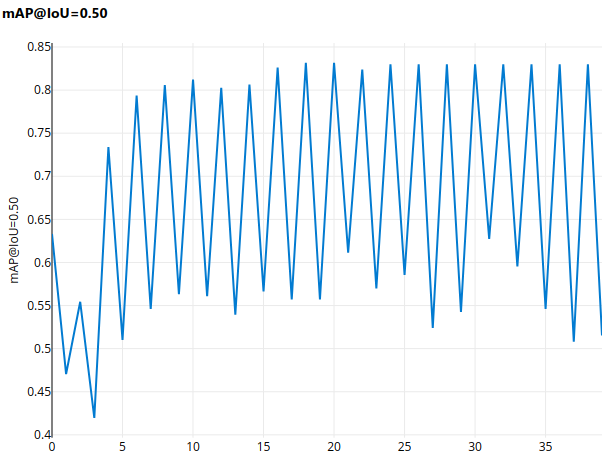
\includegraphics{image_report/metrik_friuts.png}

\hypertarget{dataset-monkeycats}{%
\paragraph{DataSet MonkeyCats}\label{dataset-monkeycats}}

\begin{verbatim}
Arguments
--data_path . --workers 8 --learning_rate 0.005 --epochs 20 --anchor_sizes
16,32,64,128,256,512 --anchor_aspect_ratios 0.25,0.5,1.0,2.0 
--rpn_nms_thresh 0.5 --box_nms_thresh 0.3 --box_score_thresh 0.1 
--num_classes 4 --dataset monkeyCats
\end{verbatim}

Czas trwania: 3h 47m 4.478s\newline
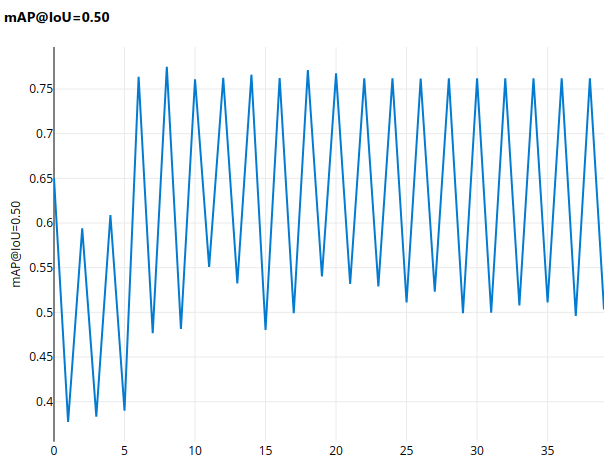
\includegraphics{image_report/metrik_monkeycats.png}

\hypertarget{dataset-playcards}{%
\paragraph{DataSet PlayCards}\label{dataset-playcards}}

\begin{verbatim}
Arguments
--data_path . --workers 8 --learning_rate 0.005 --epochs 20 --anchor_sizes
16,32,64,128,256,512 --anchor_aspect_ratios 0.25,0.5,1.0,2.0 
--rpn_nms_thresh 0.5 --box_nms_thresh 0.3 --box_score_thresh 0.1 
--num_classes 7 --dataset PlayCards
\end{verbatim}

Czas trwania: 2h 23m 4.841s\newline
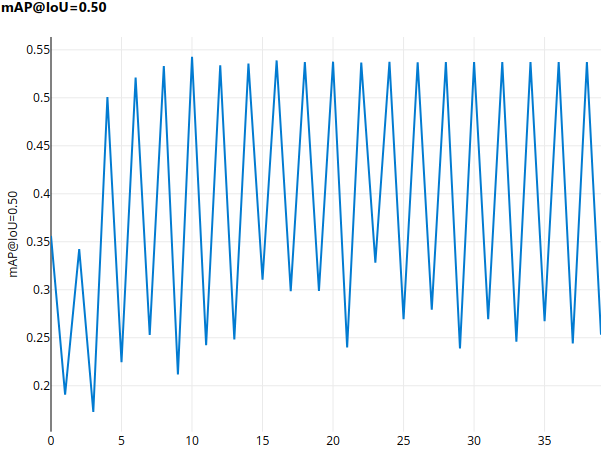
\includegraphics{image_report/metrik_cards.png}

    Poniżej pokazuje metryki wszystkich na jednym wykresie:

\textbf{93 - Fruit} \textbf{94 - MonkeyCats} \textbf{95 - PlayCards}

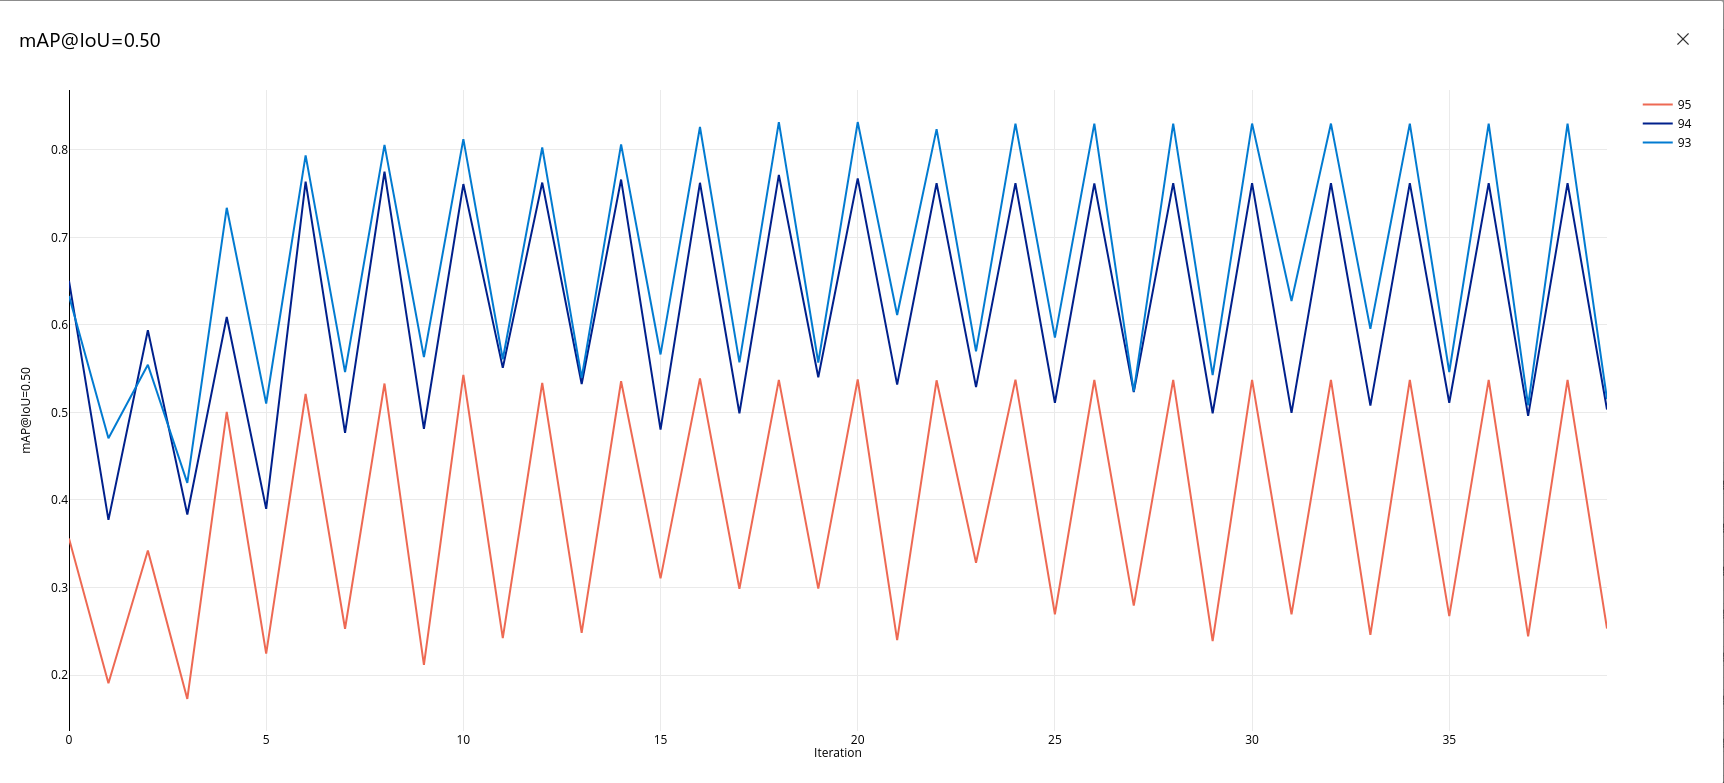
\includegraphics{image_report/metrik_all.png}

    \begin{tcolorbox}[breakable, size=fbox, boxrule=1pt, pad at break*=1mm,colback=cellbackground, colframe=cellborder]
\prompt{In}{incolor}{27}{\boxspacing}
\begin{Verbatim}[commandchars=\\\{\}]
\PY{n}{datasetsList} \PY{o}{=} \PY{p}{[}\PY{l+s+s2}{\PYZdq{}}\PY{l+s+s2}{Fruit}\PY{l+s+s2}{\PYZdq{}}\PY{p}{,}\PY{l+s+s2}{\PYZdq{}}\PY{l+s+s2}{monkeyCats}\PY{l+s+s2}{\PYZdq{}}\PY{p}{,}\PY{l+s+s2}{\PYZdq{}}\PY{l+s+s2}{PlayCards}\PY{l+s+s2}{\PYZdq{}}\PY{p}{]}
\PY{n}{classesList} \PY{o}{=} \PY{p}{[}\PY{l+m+mi}{4}\PY{p}{,}\PY{l+m+mi}{4}\PY{p}{,}\PY{l+m+mi}{7}\PY{p}{]}
\PY{n}{num\PYZus{}epochs}\PY{o}{=}\PY{l+m+mi}{20}
\PY{n}{metrics} \PY{o}{=} \PY{p}{[}\PY{p}{]}
\PY{k}{for} \PY{n}{dataset}\PY{p}{,}\PY{n}{clas} \PY{o+ow}{in} \PY{n+nb}{zip}\PY{p}{(}\PY{n}{datasetsList}\PY{p}{,}\PY{n}{classesList}\PY{p}{)}\PY{p}{:}
    \PY{n}{metrics}\PY{o}{.}\PY{n}{append}\PY{p}{(}\PY{n}{prepareEstimator} \PY{p}{(}\PY{n}{dataset}\PY{p}{,}\PY{n}{clas}\PY{p}{,}\PY{n}{num\PYZus{}epochs}\PY{p}{,}\PY{n}{dataset}\PY{p}{)}\PY{p}{)}
\end{Verbatim}
\end{tcolorbox}

    \begin{tcolorbox}[breakable, size=fbox, boxrule=1pt, pad at break*=1mm,colback=cellbackground, colframe=cellborder]
\prompt{In}{incolor}{28}{\boxspacing}
\begin{Verbatim}[commandchars=\\\{\}]
\PY{k}{with} \PY{n+nb}{open}\PY{p}{(}\PY{l+s+s1}{\PYZsq{}}\PY{l+s+s1}{metrixs.txt}\PY{l+s+s1}{\PYZsq{}}\PY{p}{,} \PY{l+s+s1}{\PYZsq{}}\PY{l+s+s1}{w}\PY{l+s+s1}{\PYZsq{}}\PY{p}{)} \PY{k}{as} \PY{n}{f}\PY{p}{:}
    \PY{k}{for} \PY{n}{item} \PY{o+ow}{in} \PY{n}{metrics}\PY{p}{:}
        \PY{n}{f}\PY{o}{.}\PY{n}{write}\PY{p}{(}\PY{l+s+s2}{\PYZdq{}}\PY{l+s+si}{\PYZpc{}s}\PY{l+s+se}{\PYZbs{}n}\PY{l+s+s2}{\PYZdq{}} \PY{o}{\PYZpc{}} \PY{n}{item}\PY{p}{)}
\end{Verbatim}
\end{tcolorbox}

    \begin{tcolorbox}[breakable, size=fbox, boxrule=1pt, pad at break*=1mm,colback=cellbackground, colframe=cellborder]
\prompt{In}{incolor}{56}{\boxspacing}
\begin{Verbatim}[commandchars=\\\{\}]
\PY{c+c1}{\PYZsh{}UWAGA! UWAGA! UWAGA!}
\end{Verbatim}
\end{tcolorbox}

    \hypertarget{dokux142adny-opis-datasetuxf3w}{%
\subsection{Dokładny opis datasetów}\label{dokux142adny-opis-datasetuxf3w}}

    \begin{tcolorbox}[breakable, size=fbox, boxrule=1pt, pad at break*=1mm,colback=cellbackground, colframe=cellborder]
\prompt{In}{incolor}{10}{\boxspacing}
\begin{Verbatim}[commandchars=\\\{\}]
\PY{k+kn}{from} \PY{n+nn}{matplotlib} \PY{k+kn}{import} \PY{n}{pyplot} \PY{k}{as} \PY{n}{plt}
\PY{k}{def} \PY{n+nf}{plotmAP}\PY{p}{(}\PY{n}{fileName}\PY{p}{,}\PY{n}{dataSets}\PY{p}{)}\PY{p}{:}
    \PY{k}{with} \PY{n+nb}{open}\PY{p}{(}\PY{n}{fileName}\PY{p}{,} \PY{l+s+s1}{\PYZsq{}}\PY{l+s+s1}{r}\PY{l+s+s1}{\PYZsq{}}\PY{p}{)} \PY{k}{as} \PY{n}{f}\PY{p}{:}
        \PY{k}{for} \PY{n}{line}\PY{p}{,} \PY{n}{title} \PY{o+ow}{in} \PY{n+nb}{zip}\PY{p}{(}\PY{n}{f}\PY{o}{.}\PY{n}{readlines}\PY{p}{(}\PY{p}{)}\PY{p}{,} \PY{n}{dataSets}\PY{p}{)}\PY{p}{:}
            \PY{n}{dic} \PY{o}{=} \PY{n+nb}{eval}\PY{p}{(}\PY{n}{line}\PY{p}{)}
            \PY{n}{plt}\PY{o}{.}\PY{n}{figure}\PY{p}{(}\PY{n}{figsize}\PY{o}{=}\PY{p}{(}\PY{l+m+mi}{10}\PY{p}{,}\PY{l+m+mi}{10}\PY{p}{)}\PY{p}{)}
            \PY{n}{plt}\PY{o}{.}\PY{n}{plot}\PY{p}{(}\PY{n}{dic}\PY{p}{[}\PY{l+s+s1}{\PYZsq{}}\PY{l+s+s1}{mAP@IoU=0.50}\PY{l+s+s1}{\PYZsq{}}\PY{p}{]}\PY{p}{[}\PY{p}{:}\PY{p}{:}\PY{l+m+mi}{2}\PY{p}{]}\PY{p}{)}
            \PY{n}{plt}\PY{o}{.}\PY{n}{plot}\PY{p}{(}\PY{n}{dic}\PY{p}{[}\PY{l+s+s1}{\PYZsq{}}\PY{l+s+s1}{mAP@IoU=0.50}\PY{l+s+s1}{\PYZsq{}}\PY{p}{]}\PY{p}{[}\PY{l+m+mi}{1}\PY{p}{:}\PY{p}{:}\PY{l+m+mi}{2}\PY{p}{]}\PY{p}{,} \PY{n}{color}\PY{o}{=}\PY{l+s+s2}{\PYZdq{}}\PY{l+s+s2}{red}\PY{l+s+s2}{\PYZdq{}}\PY{p}{)}
            \PY{n}{plt}\PY{o}{.}\PY{n}{title}\PY{p}{(}\PY{n}{title}\PY{p}{)}
            \PY{n}{plt}\PY{o}{.}\PY{n}{xlabel}\PY{p}{(}\PY{l+s+s2}{\PYZdq{}}\PY{l+s+s2}{epochs}\PY{l+s+s2}{\PYZdq{}}\PY{p}{)}
            \PY{n}{plt}\PY{o}{.}\PY{n}{ylabel}\PY{p}{(}\PY{l+s+s2}{\PYZdq{}}\PY{l+s+s2}{mAP@IoU}\PY{l+s+s2}{\PYZdq{}}\PY{p}{)}
            \PY{n}{plt}\PY{o}{.}\PY{n}{grid}\PY{p}{(}\PY{p}{)}
            \PY{n}{plt}\PY{o}{.}\PY{n}{show}\PY{p}{(}\PY{p}{)}
\end{Verbatim}
\end{tcolorbox}

    \begin{tcolorbox}[breakable, size=fbox, boxrule=1pt, pad at break*=1mm,colback=cellbackground, colframe=cellborder]
\prompt{In}{incolor}{11}{\boxspacing}
\begin{Verbatim}[commandchars=\\\{\}]
\PY{n}{plotmAP}\PY{p}{(}\PY{l+s+s2}{\PYZdq{}}\PY{l+s+s2}{metrixs\PYZhy{}1.txt}\PY{l+s+s2}{\PYZdq{}}\PY{p}{,}\PY{p}{[}\PY{l+s+s1}{\PYZsq{}}\PY{l+s+s1}{Fruits DataSet}\PY{l+s+s1}{\PYZsq{}}\PY{p}{,}  \PY{l+s+s1}{\PYZsq{}}\PY{l+s+s1}{MonkeyCats DataSet}\PY{l+s+s1}{\PYZsq{}}\PY{p}{,} \PY{l+s+s1}{\PYZsq{}}\PY{l+s+s1}{PlayCards DataSet}\PY{l+s+s1}{\PYZsq{}}\PY{p}{]}\PY{p}{)}
\end{Verbatim}
\end{tcolorbox}

    \begin{center}
    \adjustimage{max size={0.9\linewidth}{0.9\paperheight}}{image_report/output_37_0.png}
    \end{center}
    { \hspace*{\fill} \\}
    
    \begin{center}
    \adjustimage{max size={0.9\linewidth}{0.9\paperheight}}{image_report/output_37_1.png}
    \end{center}
    { \hspace*{\fill} \\}
    
    \begin{center}
    \adjustimage{max size={0.9\linewidth}{0.9\paperheight}}{image_report/output_37_2.png}
    \end{center}
    { \hspace*{\fill} \\}
    
    \begin{tcolorbox}[breakable, size=fbox, boxrule=1pt, pad at break*=1mm,colback=cellbackground, colframe=cellborder]
\prompt{In}{incolor}{16}{\boxspacing}
\begin{Verbatim}[commandchars=\\\{\}]
\PY{n}{plotmAP}\PY{p}{(}\PY{l+s+s2}{\PYZdq{}}\PY{l+s+s2}{metrixs.txt}\PY{l+s+s2}{\PYZdq{}}\PY{p}{,}\PY{p}{[}\PY{l+s+s1}{\PYZsq{}}\PY{l+s+s1}{Fruits DataSet}\PY{l+s+s1}{\PYZsq{}}\PY{p}{,}  \PY{l+s+s1}{\PYZsq{}}\PY{l+s+s1}{MonkeyCats DataSet}\PY{l+s+s1}{\PYZsq{}}\PY{p}{,} \PY{l+s+s1}{\PYZsq{}}\PY{l+s+s1}{PlayCards DataSet}\PY{l+s+s1}{\PYZsq{}}\PY{p}{]}\PY{p}{)}
\end{Verbatim}
\end{tcolorbox}

    \begin{center}
    \adjustimage{max size={0.9\linewidth}{0.9\paperheight}}{image_report/output_38_0.png}
    \end{center}
    { \hspace*{\fill} \\}
    
    \begin{center}
    \adjustimage{max size={0.9\linewidth}{0.9\paperheight}}{image_report/output_38_1.png}
    \end{center}
    { \hspace*{\fill} \\}
    
    \begin{center}
    \adjustimage{max size={0.9\linewidth}{0.9\paperheight}}{image_report/output_38_2.png}
    \end{center}
    { \hspace*{\fill} \\}
    
    \begin{tcolorbox}[breakable, size=fbox, boxrule=1pt, pad at break*=1mm,colback=cellbackground, colframe=cellborder]
\prompt{In}{incolor}{41}{\boxspacing}
\begin{Verbatim}[commandchars=\\\{\}]
\PY{k}{def} \PY{n+nf}{makePrediction}\PY{p}{(}\PY{n}{num\PYZus{}classes}\PY{p}{,}\PY{n}{dataset}\PY{p}{,}\PY{n}{model\PYZus{}path}\PY{p}{,}\PY{n}{index}\PY{p}{,}\PY{n}{labels\PYZus{}dict}\PY{p}{)}\PY{p}{:}
    \PY{n}{anchor\PYZus{}sizes} \PY{o}{=} \PY{l+s+s2}{\PYZdq{}}\PY{l+s+s2}{16,32,64,128,256,512}\PY{l+s+s2}{\PYZdq{}}
    \PY{n}{anchor\PYZus{}aspect\PYZus{}ratios} \PY{o}{=} \PY{l+s+s2}{\PYZdq{}}\PY{l+s+s2}{0.25,0.5,1.0,2.0}\PY{l+s+s2}{\PYZdq{}}
    \PY{n}{rpn\PYZus{}nms\PYZus{}threshold} \PY{o}{=} \PY{l+m+mf}{0.5}
    \PY{n}{box\PYZus{}nms\PYZus{}threshold} \PY{o}{=} \PY{l+m+mf}{0.3}
    \PY{n}{box\PYZus{}score\PYZus{}threshold} \PY{o}{=} \PY{l+m+mf}{0.1}
    \PY{n}{num\PYZus{}box\PYZus{}detections} \PY{o}{=} \PY{l+m+mi}{100}
    
    \PY{c+c1}{\PYZsh{}prepare model to make prediction}
    \PY{n}{model} \PY{o}{=} \PY{n}{get\PYZus{}model}\PY{p}{(}
        \PY{n}{num\PYZus{}classes}\PY{p}{,}
        \PY{n}{anchor\PYZus{}sizes}\PY{p}{,}
        \PY{n}{anchor\PYZus{}aspect\PYZus{}ratios}\PY{p}{,}
        \PY{n}{rpn\PYZus{}nms\PYZus{}threshold}\PY{p}{,}
        \PY{n}{box\PYZus{}nms\PYZus{}threshold}\PY{p}{,}
        \PY{n}{box\PYZus{}score\PYZus{}threshold}\PY{p}{,}
        \PY{n}{num\PYZus{}box\PYZus{}detections}\PY{p}{,}
    \PY{p}{)}
    \PY{c+c1}{\PYZsh{}model\PYZus{}path = \PYZdq{}model\PYZus{}latest.pth\PYZdq{}}
    \PY{n}{model}\PY{o}{.}\PY{n}{load\PYZus{}state\PYZus{}dict}\PY{p}{(}\PY{n}{torch}\PY{o}{.}\PY{n}{load}\PY{p}{(}\PY{n}{model\PYZus{}path}\PY{p}{)}\PY{p}{)}
    \PY{n}{device} \PY{o}{=} \PY{n}{torch}\PY{o}{.}\PY{n}{device}\PY{p}{(}\PY{l+s+s2}{\PYZdq{}}\PY{l+s+s2}{cuda}\PY{l+s+s2}{\PYZdq{}}\PY{p}{)} \PY{k}{if} \PY{n}{torch}\PY{o}{.}\PY{n}{cuda}\PY{o}{.}\PY{n}{is\PYZus{}available}\PY{p}{(}\PY{p}{)} \PY{k}{else} \PY{n}{torch}\PY{o}{.}\PY{n}{device}\PY{p}{(}\PY{l+s+s2}{\PYZdq{}}\PY{l+s+s2}{cpu}\PY{l+s+s2}{\PYZdq{}}\PY{p}{)}
    \PY{n}{model}\PY{o}{.}\PY{n}{to}\PY{p}{(}\PY{n}{device}\PY{p}{)}
    
    \PY{c+c1}{\PYZsh{} Use a random subset of the data to visualize predictions on the images.}
    \PY{n}{data\PYZus{}path} \PY{o}{=} \PY{l+s+s2}{\PYZdq{}}\PY{l+s+s2}{./scripts}\PY{l+s+s2}{\PYZdq{}}
    \PY{c+c1}{\PYZsh{}dataset = BuildDataset(data\PYZus{}path, \PYZdq{}Fruit\PYZdq{} ,get\PYZus{}transform(train=False), train=False)}
    \PY{n}{dataset} \PY{o}{=} \PY{n}{BuildDataset}\PY{p}{(}\PY{n}{data\PYZus{}path}\PY{p}{,} \PY{n}{dataset} \PY{p}{,}\PY{n}{get\PYZus{}transform}\PY{p}{(}\PY{n}{train}\PY{o}{=}\PY{k+kc}{False}\PY{p}{)}\PY{p}{,} \PY{n}{train}\PY{o}{=}\PY{k+kc}{False}\PY{p}{)}
    \PY{c+c1}{\PYZsh{}prediction}
    \PY{n}{img}\PY{p}{,} \PY{n}{\PYZus{}} \PY{o}{=} \PY{n}{dataset}\PY{p}{[}\PY{n}{index}\PY{p}{]}
    \PY{n}{model}\PY{o}{.}\PY{n}{eval}\PY{p}{(}\PY{p}{)}
    \PY{k}{with} \PY{n}{torch}\PY{o}{.}\PY{n}{no\PYZus{}grad}\PY{p}{(}\PY{p}{)}\PY{p}{:}
        \PY{n}{prediction} \PY{o}{=} \PY{n}{model}\PY{p}{(}\PY{p}{[}\PY{n}{img}\PY{o}{.}\PY{n}{to}\PY{p}{(}\PY{n}{device}\PY{p}{)}\PY{p}{]}\PY{p}{)}
    \PY{n}{img} \PY{o}{=} \PY{n}{Image}\PY{o}{.}\PY{n}{fromarray}\PY{p}{(}\PY{n}{img}\PY{o}{.}\PY{n}{mul}\PY{p}{(}\PY{l+m+mi}{255}\PY{p}{)}\PY{o}{.}\PY{n}{permute}\PY{p}{(}\PY{l+m+mi}{1}\PY{p}{,} \PY{l+m+mi}{2}\PY{p}{,} \PY{l+m+mi}{0}\PY{p}{)}\PY{o}{.}\PY{n}{byte}\PY{p}{(}\PY{p}{)}\PY{o}{.}\PY{n}{numpy}\PY{p}{(}\PY{p}{)}\PY{p}{)}
    \PY{n}{preds} \PY{o}{=} \PY{n}{prediction}\PY{p}{[}\PY{l+m+mi}{0}\PY{p}{]}\PY{p}{[}\PY{l+s+s2}{\PYZdq{}}\PY{l+s+s2}{boxes}\PY{l+s+s2}{\PYZdq{}}\PY{p}{]}\PY{o}{.}\PY{n}{cpu}\PY{p}{(}\PY{p}{)}\PY{o}{.}\PY{n}{numpy}\PY{p}{(}\PY{p}{)}
    \PY{n+nb}{print}\PY{p}{(}\PY{n}{prediction}\PY{p}{[}\PY{l+m+mi}{0}\PY{p}{]}\PY{p}{[}\PY{l+s+s2}{\PYZdq{}}\PY{l+s+s2}{scores}\PY{l+s+s2}{\PYZdq{}}\PY{p}{]}\PY{p}{)}
    \PY{n+nb}{print}\PY{p}{(}\PY{n}{prediction}\PY{p}{[}\PY{l+m+mi}{0}\PY{p}{]}\PY{p}{[}\PY{l+s+s1}{\PYZsq{}}\PY{l+s+s1}{labels}\PY{l+s+s1}{\PYZsq{}}\PY{p}{]}\PY{p}{)}
    \PY{n}{draw} \PY{o}{=} \PY{n}{ImageDraw}\PY{o}{.}\PY{n}{Draw}\PY{p}{(}\PY{n}{img}\PY{p}{)}
    \PY{k}{for} \PY{n}{i} \PY{o+ow}{in} \PY{n+nb}{range}\PY{p}{(}\PY{n+nb}{len}\PY{p}{(}\PY{n}{preds}\PY{p}{)}\PY{p}{)}\PY{p}{:}
        \PY{k}{if} \PY{n}{prediction}\PY{p}{[}\PY{l+m+mi}{0}\PY{p}{]}\PY{p}{[}\PY{l+s+s2}{\PYZdq{}}\PY{l+s+s2}{scores}\PY{l+s+s2}{\PYZdq{}}\PY{p}{]}\PY{p}{[}\PY{n}{i}\PY{p}{]}\PY{o}{.}\PY{n}{item}\PY{p}{(}\PY{p}{)} \PY{o}{\PYZgt{}} \PY{l+m+mf}{0.5}\PY{p}{:}
            \PY{n}{draw}\PY{o}{.}\PY{n}{rectangle}\PY{p}{(}
                \PY{p}{(}\PY{p}{(}\PY{n}{preds}\PY{p}{[}\PY{n}{i}\PY{p}{]}\PY{p}{[}\PY{l+m+mi}{0}\PY{p}{]}\PY{p}{,} \PY{n}{preds}\PY{p}{[}\PY{n}{i}\PY{p}{]}\PY{p}{[}\PY{l+m+mi}{1}\PY{p}{]}\PY{p}{)}\PY{p}{,} \PY{p}{(}\PY{n}{preds}\PY{p}{[}\PY{n}{i}\PY{p}{]}\PY{p}{[}\PY{l+m+mi}{2}\PY{p}{]}\PY{p}{,} \PY{n}{preds}\PY{p}{[}\PY{n}{i}\PY{p}{]}\PY{p}{[}\PY{l+m+mi}{3}\PY{p}{]}\PY{p}{)}\PY{p}{)}\PY{p}{,} \PY{n}{outline}\PY{o}{=}\PY{l+s+s2}{\PYZdq{}}\PY{l+s+s2}{red}\PY{l+s+s2}{\PYZdq{}}
            \PY{p}{)}
            \PY{n}{draw}\PY{o}{.}\PY{n}{text}\PY{p}{(}\PY{p}{(}\PY{n}{preds}\PY{p}{[}\PY{n}{i}\PY{p}{]}\PY{p}{[}\PY{l+m+mi}{0}\PY{p}{]}\PY{p}{,} \PY{n}{preds}\PY{p}{[}\PY{n}{i}\PY{p}{]}\PY{p}{[}\PY{l+m+mi}{1}\PY{p}{]}\PY{p}{)}\PY{p}{,} \PY{n}{labels\PYZus{}dict}\PY{p}{[}\PY{n}{prediction}\PY{p}{[}\PY{l+m+mi}{0}\PY{p}{]}\PY{p}{[}\PY{l+s+s1}{\PYZsq{}}\PY{l+s+s1}{labels}\PY{l+s+s1}{\PYZsq{}}\PY{p}{]}\PY{p}{[}\PY{n}{i}\PY{p}{]}\PY{o}{.}\PY{n}{item}\PY{p}{(}\PY{p}{)}\PY{p}{]}\PY{p}{,} \PY{n}{fill}\PY{o}{=}\PY{p}{(}\PY{l+m+mi}{52}\PY{p}{,} \PY{l+m+mi}{55}\PY{p}{,} \PY{l+m+mi}{235}\PY{p}{,}\PY{l+m+mi}{128}\PY{p}{)}\PY{p}{)}
    \PY{n}{display}\PY{p}{(}\PY{n}{img}\PY{p}{)}
\end{Verbatim}
\end{tcolorbox}

    \hypertarget{poruxf3wnanie-mask-r-cnn-z-custom-vision}{%
\section{Porównanie Mask R-CNN z Custom
Vision}\label{poruxf3wnanie-mask-r-cnn-z-custom-vision}}

\hypertarget{dataset-fruits}{%
\subsection{Dataset Fruits}\label{dataset-fruits}}

Po wytrenowaniu Custom Vision otrzymaliśmy takie wyniki dla datasetu
Fruits: 
\begin{itemize}
    \item \textbf{Precision} - jak prawdopodobne jest, że jest to
prawda?
\item \textbf{Recall} - spośród tagów, które należy prawidłowo
przewidzieć, jaki procent poprawnie znalazł twój model?
\item \textbf{mAP} -
(średnia dokładność) ogólna wydajność detektora obiektów we wszystkich
znacznikach
\end{itemize}
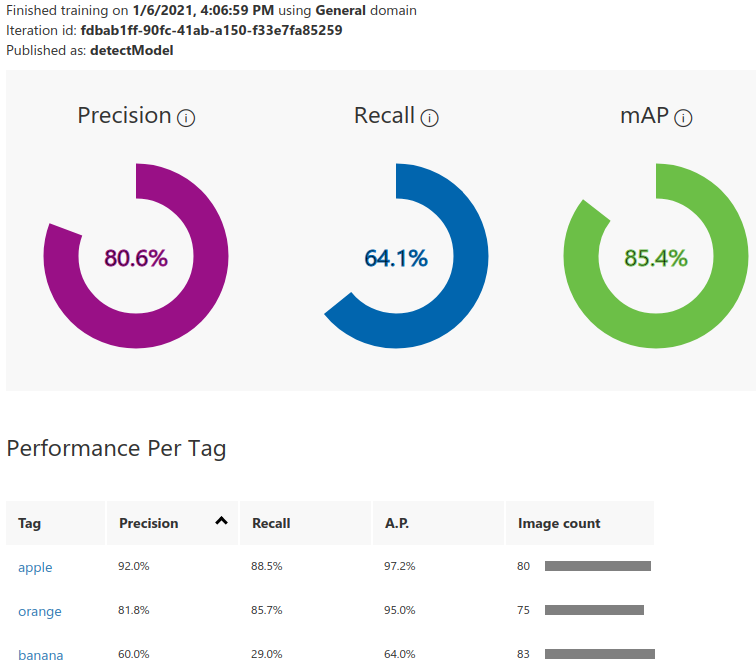
\includegraphics{image_report/custom_fruits.png}

    Przykład wykrywania obiektu na zdjęciu. Jest pokazane, że to jest banan.

    \hypertarget{custom-vision}{%
\subsubsection{Custom Vision}\label{custom-vision}}

Zdjęcie dla Custom Vision:\newline
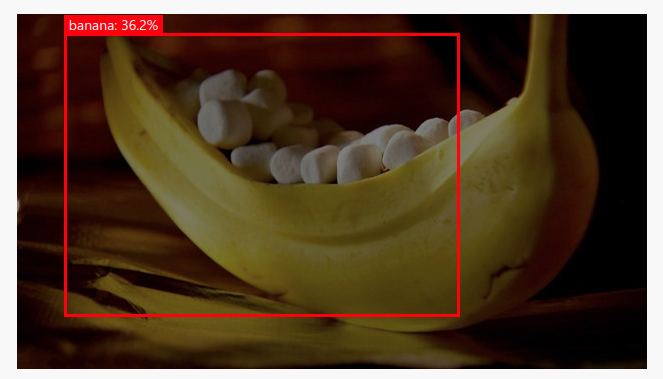
\includegraphics{image_report/custom_fruits_1.png} \newline
Predition:\newline
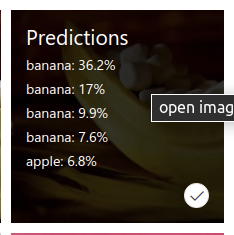
\includegraphics{image_report/custom_fruits_2.png}\newline

    \hypertarget{mask-r-cnn}{%
\subsubsection{Mask R-CNN}\label{mask-r-cnn}}

    \begin{tcolorbox}[breakable, size=fbox, boxrule=1pt, pad at break*=1mm,colback=cellbackground, colframe=cellborder]
\prompt{In}{incolor}{42}{\boxspacing}
\begin{Verbatim}[commandchars=\\\{\}]
\PY{c+c1}{\PYZsh{}Można pobawić się z predykcją}
\PY{n}{labels\PYZus{}dict} \PY{o}{=} \PY{p}{\PYZob{}}\PY{l+m+mi}{1}\PY{p}{:} \PY{l+s+s1}{\PYZsq{}}\PY{l+s+s1}{apple}\PY{l+s+s1}{\PYZsq{}}\PY{p}{,} \PY{l+m+mi}{2}\PY{p}{:} \PY{l+s+s1}{\PYZsq{}}\PY{l+s+s1}{orange}\PY{l+s+s1}{\PYZsq{}}\PY{p}{,} \PY{l+m+mi}{3}\PY{p}{:} \PY{l+s+s1}{\PYZsq{}}\PY{l+s+s1}{banana}\PY{l+s+s1}{\PYZsq{}}\PY{p}{\PYZcb{}}
\PY{n}{makePrediction}\PY{p}{(}\PY{l+m+mi}{4}\PY{p}{,}\PY{l+s+s2}{\PYZdq{}}\PY{l+s+s2}{Fruit}\PY{l+s+s2}{\PYZdq{}}\PY{p}{,}\PY{l+s+s2}{\PYZdq{}}\PY{l+s+s2}{Fruitmodel\PYZus{}latest.pth}\PY{l+s+s2}{\PYZdq{}}\PY{p}{,}\PY{l+m+mi}{25}\PY{p}{,}\PY{n}{labels\PYZus{}dict}\PY{p}{)}
\end{Verbatim}
\end{tcolorbox}

    \begin{Verbatim}[commandchars=\\\{\}]
tensor([0.8869, 0.4075, 0.2982], device='cuda:0')
tensor([3, 1, 3], device='cuda:0')
    \end{Verbatim}

    \begin{center}
    \adjustimage{max size={0.9\linewidth}{0.9\paperheight}}{image_report/output_44_1.png}
    \end{center}
    { \hspace*{\fill} \\}
    
    \hypertarget{wnioski-z-przykux142adu}{%
\subsubsection{Wnioski z przykładu}\label{wnioski-z-przykux142adu}}

Zdjęcie z bananem wyszło nam, że dla Custom Vision jest 36.2\%
prawdopodobieństwa, natomiast dla Mask R-CNN wychodzi 88.69\%
prawdopodobeństwa.

\textbf{W tym wypadku Mask R-CNN pokazał siebie z lepszej strony}

    \hypertarget{dataset-monkey-cat-dog}{%
\subsection{Dataset Monkey Cat Dog}\label{dataset-monkey-cat-dog}}

Po wytrenowaniu Custom Vision otrzymaliśmy takie wyniki dla datasetu
Monkey Cat Dog: 
\begin{itemize}
    \item \textbf{Precision} - jak prawdopodobne jest, że jest to
prawda?
\item \textbf{Recall} - spośród tagów, które należy prawidłowo
przewidzieć, jaki procent poprawnie znalazł twój model?
\item \textbf{mAP} -
(średnia dokładność) ogólna wydajność detektora obiektów we wszystkich
znacznikach
\end{itemize}
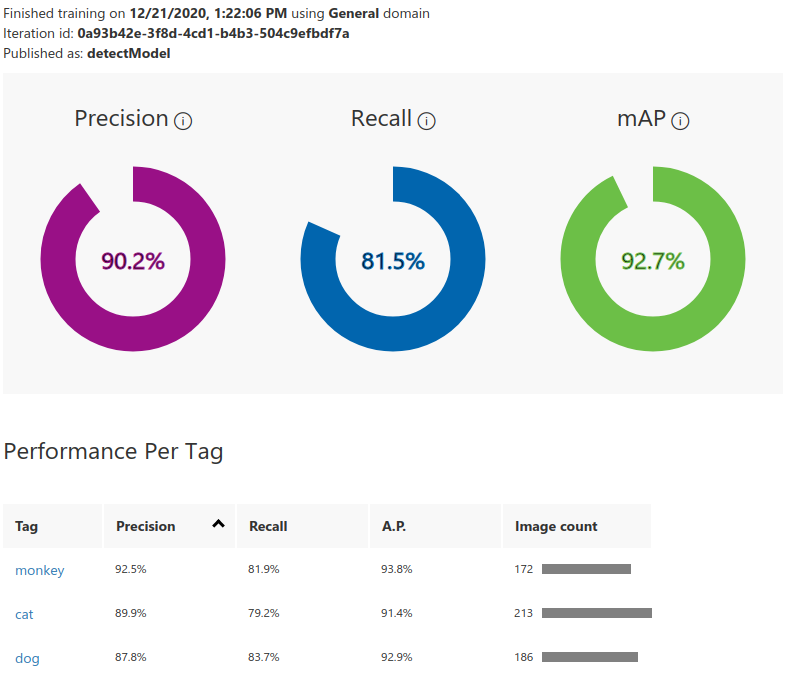
\includegraphics{image_report/custom_monkey.png}

    \hypertarget{custom-vision}{%
\subsubsection{Custom Vision}\label{custom-vision}}

Zdjęcie dla Custom Vision:\newline
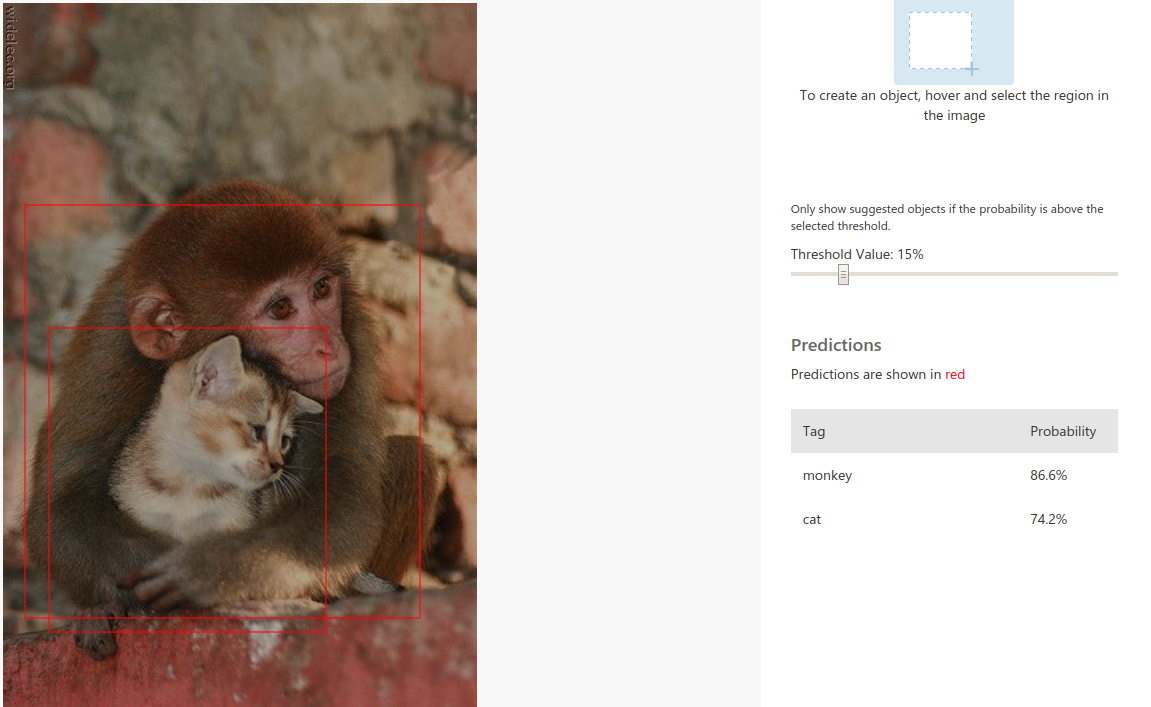
\includegraphics{image_report/custom_monkey_1.png} \newline
Predition:\newline
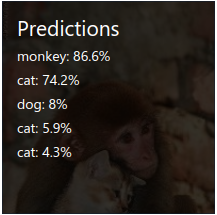
\includegraphics{image_report/custom_monkey_2.png}

    \hypertarget{mask-r-cnn}{%
\subsubsection{Mask R-CNN}\label{mask-r-cnn}}

    \begin{tcolorbox}[breakable, size=fbox, boxrule=1pt, pad at break*=1mm,colback=cellbackground, colframe=cellborder]
\prompt{In}{incolor}{45}{\boxspacing}
\begin{Verbatim}[commandchars=\\\{\}]
\PY{n}{labels\PYZus{}dict} \PY{o}{=} \PY{p}{\PYZob{}}\PY{l+m+mi}{1}\PY{p}{:} \PY{l+s+s2}{\PYZdq{}}\PY{l+s+s2}{cat}\PY{l+s+s2}{\PYZdq{}}\PY{p}{,} \PY{l+m+mi}{2}\PY{p}{:} \PY{l+s+s2}{\PYZdq{}}\PY{l+s+s2}{dog}\PY{l+s+s2}{\PYZdq{}}\PY{p}{,} \PY{l+m+mi}{3}\PY{p}{:} \PY{l+s+s2}{\PYZdq{}}\PY{l+s+s2}{monkey}\PY{l+s+s2}{\PYZdq{}}\PY{p}{\PYZcb{}}
\PY{n}{makePrediction}\PY{p}{(}\PY{l+m+mi}{4}\PY{p}{,}\PY{l+s+s2}{\PYZdq{}}\PY{l+s+s2}{monkeyCats}\PY{l+s+s2}{\PYZdq{}}\PY{p}{,}\PY{l+s+s2}{\PYZdq{}}\PY{l+s+s2}{monkeyCatsmodel\PYZus{}latest1.pth}\PY{l+s+s2}{\PYZdq{}}\PY{p}{,}\PY{l+m+mi}{11}\PY{p}{,}\PY{n}{labels\PYZus{}dict}\PY{p}{)}
\end{Verbatim}
\end{tcolorbox}

    \begin{Verbatim}[commandchars=\\\{\}]
tensor([0.9081, 0.4157], device='cuda:0')
tensor([3, 1], device='cuda:0')
    \end{Verbatim}

    \begin{center}
    \adjustimage{max size={0.9\linewidth}{0.9\paperheight}}{image_report/output_49_1.png}
    \end{center}
    { \hspace*{\fill} \\}
    
    \hypertarget{wnioski-z-przykux142adu}) a małpa(\textbf{86.6\%}) prawdopodobieństwa,
natomiast dla Mask R-CNN nie wykrył w ogóle kota, a tylko
małpę(\textbf{90\%})

\textbf{W tym wypadku Custom Vision pokazał siebie z lepszej strony}
Czyli dla wykrywanie jednego obiektu na zdjęciu radzi sobie lepiej Mask
R-CNN, natomiast Custom Vision wykrawa lepiej zdjęcia z dwoma lub więcej
obiektami.

    \hypertarget{dataset-play-cards}{%
\subsection{Dataset Play Cards}\label{dataset-play-cards}}

Po wytrenowaniu Custom Vision otrzymaliśmy takie wyniki dla datasetu
Play Cards:
\begin{itemize}
    \item \textbf{Precision} - jak prawdopodobne jest, że jest to
prawda?
\item \textbf{Recall} - spośród tagów, które należy prawidłowo
przewidzieć, jaki procent poprawnie znalazł twój model?
\item \textbf{mAP} -
(średnia dokładność) ogólna wydajność detektora obiektów we wszystkich
znacznikach
\end{itemize}

    \hypertarget{mask-r-cnn}{%
\subsubsection{Mask R-CNN}\label{mask-r-cnn}}



    \begin{tcolorbox}[breakable, size=fbox, boxrule=1pt, pad at break*=1mm,colback=cellbackground, colframe=cellborder]
\prompt{In}{incolor}{54}{\boxspacing}
\begin{Verbatim}[commandchars=\\\{\}]
\PY{n}{labels\PYZus{}dict} \PY{o}{=} \PY{p}{\PYZob{}}\PY{l+m+mi}{1}\PY{p}{:} \PY{l+s+s1}{\PYZsq{}}\PY{l+s+s1}{ace}\PY{l+s+s1}{\PYZsq{}}\PY{p}{,} \PY{l+m+mi}{2}\PY{p}{:} \PY{l+s+s1}{\PYZsq{}}\PY{l+s+s1}{king}\PY{l+s+s1}{\PYZsq{}}\PY{p}{,} \PY{l+m+mi}{3}\PY{p}{:} \PY{l+s+s1}{\PYZsq{}}\PY{l+s+s1}{queen}\PY{l+s+s1}{\PYZsq{}}\PY{p}{,} \PY{l+m+mi}{4}\PY{p}{:} \PY{l+s+s1}{\PYZsq{}}\PY{l+s+s1}{jack}\PY{l+s+s1}{\PYZsq{}}\PY{p}{,} \PY{l+m+mi}{5}\PY{p}{:} \PY{l+s+s1}{\PYZsq{}}\PY{l+s+s1}{ten}\PY{l+s+s1}{\PYZsq{}}\PY{p}{,} \PY{l+m+mi}{6}\PY{p}{:} \PY{l+s+s1}{\PYZsq{}}\PY{l+s+s1}{nine}\PY{l+s+s1}{\PYZsq{}}\PY{p}{\PYZcb{}}
\PY{n}{makePrediction}\PY{p}{(}\PY{l+m+mi}{7}\PY{p}{,}\PY{l+s+s2}{\PYZdq{}}\PY{l+s+s2}{PlayCards}\PY{l+s+s2}{\PYZdq{}}\PY{p}{,}\PY{l+s+s2}{\PYZdq{}}\PY{l+s+s2}{PlayCardsmodel\PYZus{}latest1.pth}\PY{l+s+s2}{\PYZdq{}}\PY{p}{,}\PY{l+m+mi}{55}\PY{p}{,}\PY{n}{labels\PYZus{}dict}\PY{p}{)}
\end{Verbatim}
\end{tcolorbox}

    \begin{Verbatim}[commandchars=\\\{\}]
tensor([0.8226, 0.5251, 0.1733, 0.1463], device='cuda:0')
tensor([1, 1, 5, 6], device='cuda:0')
    \end{Verbatim}

    \begin{center}
    \adjustimage{max size={0.9\linewidth}{0.9\paperheight}}{image_report/output_54_1.png}
    \end{center}
    { \hspace*{\fill} \\}
    \hypertarget{wnioski-z-przykux142adu}{%
\subsubsection{Wnioski z przykładu}\label{wnioski-z-przykux142adu}}

Na zbiorze danych Play Cards wykryło dwa asy ( czyli pozytywnie). Z
powodu zmiany predykcji z 4 na 7.    
    

    \begin{tcolorbox}[breakable, size=fbox, boxrule=1pt, pad at break*=1mm,colback=cellbackground, colframe=cellborder]
\prompt{In}{incolor}{14}{\boxspacing}
\begin{Verbatim}[commandchars=\\\{\}]
\PY{n}{num\PYZus{}classes} \PY{o}{=} \PY{l+m+mi}{4}
\PY{n}{anchor\PYZus{}sizes} \PY{o}{=} \PY{l+s+s2}{\PYZdq{}}\PY{l+s+s2}{16,32,64,128,256,512}\PY{l+s+s2}{\PYZdq{}}
\PY{n}{anchor\PYZus{}aspect\PYZus{}ratios} \PY{o}{=} \PY{l+s+s2}{\PYZdq{}}\PY{l+s+s2}{0.25,0.5,1.0,2.0}\PY{l+s+s2}{\PYZdq{}}
\PY{n}{rpn\PYZus{}nms\PYZus{}threshold} \PY{o}{=} \PY{l+m+mf}{0.5}
\PY{n}{box\PYZus{}nms\PYZus{}threshold} \PY{o}{=} \PY{l+m+mf}{0.3}
\PY{n}{box\PYZus{}score\PYZus{}threshold} \PY{o}{=} \PY{l+m+mf}{0.1}
\PY{n}{num\PYZus{}box\PYZus{}detections} \PY{o}{=} \PY{l+m+mi}{100}
\end{Verbatim}
\end{tcolorbox}

    \begin{tcolorbox}[breakable, size=fbox, boxrule=1pt, pad at break*=1mm,colback=cellbackground, colframe=cellborder]
\prompt{In}{incolor}{15}{\boxspacing}
\begin{Verbatim}[commandchars=\\\{\}]
\PY{c+c1}{\PYZsh{} Load Mask RCNN model}
\PY{n}{model} \PY{o}{=} \PY{n}{get\PYZus{}model}\PY{p}{(}
    \PY{n}{num\PYZus{}classes}\PY{p}{,}
    \PY{n}{anchor\PYZus{}sizes}\PY{p}{,}
    \PY{n}{anchor\PYZus{}aspect\PYZus{}ratios}\PY{p}{,}
    \PY{n}{rpn\PYZus{}nms\PYZus{}threshold}\PY{p}{,}
    \PY{n}{box\PYZus{}nms\PYZus{}threshold}\PY{p}{,}
    \PY{n}{box\PYZus{}score\PYZus{}threshold}\PY{p}{,}
    \PY{n}{num\PYZus{}box\PYZus{}detections}\PY{p}{,}
\PY{p}{)}
\end{Verbatim}
\end{tcolorbox}

    \begin{tcolorbox}[breakable, size=fbox, boxrule=1pt, pad at break*=1mm,colback=cellbackground, colframe=cellborder]
\prompt{In}{incolor}{16}{\boxspacing}
\begin{Verbatim}[commandchars=\\\{\}]
\PY{n}{model\PYZus{}path} \PY{o}{=} \PY{l+s+s2}{\PYZdq{}}\PY{l+s+s2}{model\PYZus{}latest.pth}\PY{l+s+s2}{\PYZdq{}}
\PY{n}{model}\PY{o}{.}\PY{n}{load\PYZus{}state\PYZus{}dict}\PY{p}{(}\PY{n}{torch}\PY{o}{.}\PY{n}{load}\PY{p}{(}\PY{n}{model\PYZus{}path}\PY{p}{)}\PY{p}{)}
\PY{n}{device} \PY{o}{=} \PY{n}{torch}\PY{o}{.}\PY{n}{device}\PY{p}{(}\PY{l+s+s2}{\PYZdq{}}\PY{l+s+s2}{cuda}\PY{l+s+s2}{\PYZdq{}}\PY{p}{)} \PY{k}{if} \PY{n}{torch}\PY{o}{.}\PY{n}{cuda}\PY{o}{.}\PY{n}{is\PYZus{}available}\PY{p}{(}\PY{p}{)} \PY{k}{else} \PY{n}{torch}\PY{o}{.}\PY{n}{device}\PY{p}{(}\PY{l+s+s2}{\PYZdq{}}\PY{l+s+s2}{cpu}\PY{l+s+s2}{\PYZdq{}}\PY{p}{)}
\PY{n}{model}\PY{o}{.}\PY{n}{to}\PY{p}{(}\PY{n}{device}\PY{p}{)}
\end{Verbatim}
\end{tcolorbox}

    \begin{tcolorbox}[breakable, size=fbox, boxrule=1pt, pad at break*=1mm,colback=cellbackground, colframe=cellborder]
\prompt{In}{incolor}{17}{\boxspacing}
\begin{Verbatim}[commandchars=\\\{\}]
\PY{c+c1}{\PYZsh{} Use a random subset of the data to visualize predictions on the images.}
\PY{n}{data\PYZus{}path} \PY{o}{=} \PY{l+s+s2}{\PYZdq{}}\PY{l+s+s2}{./scripts}\PY{l+s+s2}{\PYZdq{}}
\PY{n}{dataset} \PY{o}{=} \PY{n}{BuildDataset}\PY{p}{(}\PY{n}{data\PYZus{}path}\PY{p}{,} \PY{l+s+s2}{\PYZdq{}}\PY{l+s+s2}{Fruit}\PY{l+s+s2}{\PYZdq{}} \PY{p}{,}\PY{n}{get\PYZus{}transform}\PY{p}{(}\PY{n}{train}\PY{o}{=}\PY{k+kc}{False}\PY{p}{)}\PY{p}{,} \PY{n}{train}\PY{o}{=}\PY{k+kc}{False}\PY{p}{)}
\PY{c+c1}{\PYZsh{} indices = torch.randperm(len(dataset)).tolist()}
\PY{c+c1}{\PYZsh{} dataset = torch.utils.data.Subset(dataset, indices[\PYZhy{}50:])}
\end{Verbatim}
\end{tcolorbox}

    \begin{tcolorbox}[breakable, size=fbox, boxrule=1pt, pad at break*=1mm,colback=cellbackground, colframe=cellborder]
\prompt{In}{incolor}{18}{\boxspacing}
\begin{Verbatim}[commandchars=\\\{\}]
\PY{c+c1}{\PYZsh{} for i in range(5):}
\PY{c+c1}{\PYZsh{}     img, \PYZus{} = dataset[i]}
\PY{c+c1}{\PYZsh{}     model.eval()}
\PY{c+c1}{\PYZsh{}     with torch.no\PYZus{}grad():}
\PY{c+c1}{\PYZsh{}         prediction = model([img.to(device)])}
\PY{c+c1}{\PYZsh{}     img = Image.fromarray(img.mul(255).permute(1, 2, 0).byte().numpy())}
\PY{c+c1}{\PYZsh{}     preds = prediction[0][\PYZdq{}boxes\PYZdq{}].cpu().numpy()}
\PY{c+c1}{\PYZsh{}     print(prediction[0][\PYZdq{}scores\PYZdq{}])}
\PY{c+c1}{\PYZsh{}     draw = ImageDraw.Draw(img)}
\PY{c+c1}{\PYZsh{}     for i in range(len(preds)):}
\PY{c+c1}{\PYZsh{}         draw.rectangle(}
\PY{c+c1}{\PYZsh{}             ((preds[i][0], preds[i][1]), (preds[i][2], preds[i][3])), outline=\PYZdq{}red\PYZdq{}}
\PY{c+c1}{\PYZsh{}         )}
\PY{c+c1}{\PYZsh{}     display(img)}
\end{Verbatim}
\end{tcolorbox}

    \begin{tcolorbox}[breakable, size=fbox, boxrule=1pt, pad at break*=1mm,colback=cellbackground, colframe=cellborder]
\prompt{In}{incolor}{19}{\boxspacing}
\begin{Verbatim}[commandchars=\\\{\}]
\PY{n}{img}\PY{p}{,} \PY{n}{\PYZus{}} \PY{o}{=} \PY{n}{dataset}\PY{p}{[}\PY{l+m+mi}{1}\PY{p}{]}
\PY{n}{model}\PY{o}{.}\PY{n}{eval}\PY{p}{(}\PY{p}{)}
\PY{k}{with} \PY{n}{torch}\PY{o}{.}\PY{n}{no\PYZus{}grad}\PY{p}{(}\PY{p}{)}\PY{p}{:}
    \PY{n}{prediction} \PY{o}{=} \PY{n}{model}\PY{p}{(}\PY{p}{[}\PY{n}{img}\PY{o}{.}\PY{n}{to}\PY{p}{(}\PY{n}{device}\PY{p}{)}\PY{p}{]}\PY{p}{)}
\PY{n}{img} \PY{o}{=} \PY{n}{Image}\PY{o}{.}\PY{n}{fromarray}\PY{p}{(}\PY{n}{img}\PY{o}{.}\PY{n}{mul}\PY{p}{(}\PY{l+m+mi}{255}\PY{p}{)}\PY{o}{.}\PY{n}{permute}\PY{p}{(}\PY{l+m+mi}{1}\PY{p}{,} \PY{l+m+mi}{2}\PY{p}{,} \PY{l+m+mi}{0}\PY{p}{)}\PY{o}{.}\PY{n}{byte}\PY{p}{(}\PY{p}{)}\PY{o}{.}\PY{n}{numpy}\PY{p}{(}\PY{p}{)}\PY{p}{)}
\PY{n}{preds} \PY{o}{=} \PY{n}{prediction}\PY{p}{[}\PY{l+m+mi}{0}\PY{p}{]}\PY{p}{[}\PY{l+s+s2}{\PYZdq{}}\PY{l+s+s2}{boxes}\PY{l+s+s2}{\PYZdq{}}\PY{p}{]}\PY{o}{.}\PY{n}{cpu}\PY{p}{(}\PY{p}{)}\PY{o}{.}\PY{n}{numpy}\PY{p}{(}\PY{p}{)}
\PY{n+nb}{print}\PY{p}{(}\PY{n}{prediction}\PY{p}{[}\PY{l+m+mi}{0}\PY{p}{]}\PY{p}{)}
\end{Verbatim}
\end{tcolorbox}

    \begin{Verbatim}[commandchars=\\\{\}]
\{'boxes': tensor([[  9.2525,  24.6268, 350.0000, 340.1003]], device='cuda:0'),
'labels': tensor([1], device='cuda:0'), 'scores': tensor([0.6061],
device='cuda:0')\}
    \end{Verbatim}

    \begin{tcolorbox}[breakable, size=fbox, boxrule=1pt, pad at break*=1mm,colback=cellbackground, colframe=cellborder]
\prompt{In}{incolor}{20}{\boxspacing}
\begin{Verbatim}[commandchars=\\\{\}]
\PY{n}{labels\PYZus{}dict} \PY{o}{=} \PY{p}{\PYZob{}}\PY{l+m+mi}{1}\PY{p}{:} \PY{l+s+s1}{\PYZsq{}}\PY{l+s+s1}{apple}\PY{l+s+s1}{\PYZsq{}}\PY{p}{,} \PY{l+m+mi}{2}\PY{p}{:} \PY{l+s+s1}{\PYZsq{}}\PY{l+s+s1}{orange}\PY{l+s+s1}{\PYZsq{}}\PY{p}{,} \PY{l+m+mi}{3}\PY{p}{:} \PY{l+s+s1}{\PYZsq{}}\PY{l+s+s1}{banana}\PY{l+s+s1}{\PYZsq{}}\PY{p}{\PYZcb{}}

\PY{c+c1}{\PYZsh{}labels\PYZus{}dict = \PYZob{}1: \PYZsq{}ace\PYZsq{}, 2: \PYZsq{}king\PYZsq{}, 3: \PYZsq{}queen\PYZsq{}, 4: \PYZsq{}jack\PYZsq{}, 5: \PYZsq{}ten\PYZsq{}, 6: \PYZsq{}nine\PYZsq{}\PYZcb{}}

\PY{c+c1}{\PYZsh{}labels\PYZus{}dict = \PYZob{}1: \PYZdq{}cat\PYZdq{}, 2: \PYZdq{}dog\PYZdq{}, 3: \PYZdq{}monkey\PYZdq{}\PYZcb{}}
\end{Verbatim}
\end{tcolorbox}

    \hypertarget{custom-vision}{%
\subsubsection{Custom Vision}\label{custom-vision}}

Zdjęcie dla Custom Vision: \newline
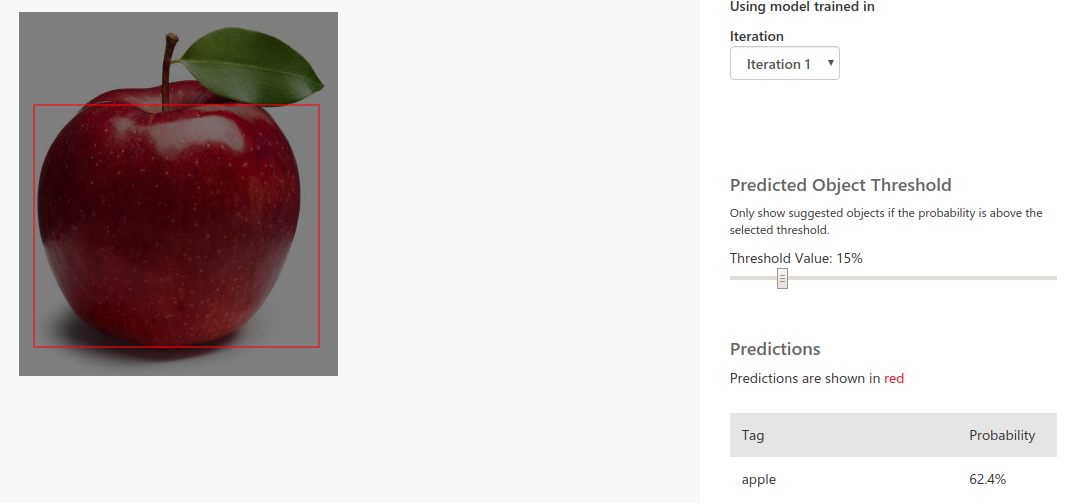
\includegraphics{image_report/apple_89.png}

    \begin{tcolorbox}[breakable, size=fbox, boxrule=1pt, pad at break*=1mm,colback=cellbackground, colframe=cellborder]
\prompt{In}{incolor}{21}{\boxspacing}
\begin{Verbatim}[commandchars=\\\{\}]
\PY{n}{img}\PY{p}{,} \PY{n}{\PYZus{}} \PY{o}{=} \PY{n}{dataset}\PY{p}{[}\PY{l+m+mi}{12}\PY{p}{]}
\PY{n}{model}\PY{o}{.}\PY{n}{eval}\PY{p}{(}\PY{p}{)}
\PY{k}{with} \PY{n}{torch}\PY{o}{.}\PY{n}{no\PYZus{}grad}\PY{p}{(}\PY{p}{)}\PY{p}{:}
    \PY{n}{prediction} \PY{o}{=} \PY{n}{model}\PY{p}{(}\PY{p}{[}\PY{n}{img}\PY{o}{.}\PY{n}{to}\PY{p}{(}\PY{n}{device}\PY{p}{)}\PY{p}{]}\PY{p}{)}
\PY{n}{img} \PY{o}{=} \PY{n}{Image}\PY{o}{.}\PY{n}{fromarray}\PY{p}{(}\PY{n}{img}\PY{o}{.}\PY{n}{mul}\PY{p}{(}\PY{l+m+mi}{255}\PY{p}{)}\PY{o}{.}\PY{n}{permute}\PY{p}{(}\PY{l+m+mi}{1}\PY{p}{,} \PY{l+m+mi}{2}\PY{p}{,} \PY{l+m+mi}{0}\PY{p}{)}\PY{o}{.}\PY{n}{byte}\PY{p}{(}\PY{p}{)}\PY{o}{.}\PY{n}{numpy}\PY{p}{(}\PY{p}{)}\PY{p}{)}
\PY{n}{preds} \PY{o}{=} \PY{n}{prediction}\PY{p}{[}\PY{l+m+mi}{0}\PY{p}{]}\PY{p}{[}\PY{l+s+s2}{\PYZdq{}}\PY{l+s+s2}{boxes}\PY{l+s+s2}{\PYZdq{}}\PY{p}{]}\PY{o}{.}\PY{n}{cpu}\PY{p}{(}\PY{p}{)}\PY{o}{.}\PY{n}{numpy}\PY{p}{(}\PY{p}{)}
\PY{n+nb}{print}\PY{p}{(}\PY{n}{prediction}\PY{p}{[}\PY{l+m+mi}{0}\PY{p}{]}\PY{p}{[}\PY{l+s+s2}{\PYZdq{}}\PY{l+s+s2}{scores}\PY{l+s+s2}{\PYZdq{}}\PY{p}{]}\PY{p}{)}
\PY{n+nb}{print}\PY{p}{(}\PY{n}{prediction}\PY{p}{[}\PY{l+m+mi}{0}\PY{p}{]}\PY{p}{[}\PY{l+s+s1}{\PYZsq{}}\PY{l+s+s1}{labels}\PY{l+s+s1}{\PYZsq{}}\PY{p}{]}\PY{p}{)}
\PY{n}{draw} \PY{o}{=} \PY{n}{ImageDraw}\PY{o}{.}\PY{n}{Draw}\PY{p}{(}\PY{n}{img}\PY{p}{)}
\PY{k}{for} \PY{n}{i} \PY{o+ow}{in} \PY{n+nb}{range}\PY{p}{(}\PY{n+nb}{len}\PY{p}{(}\PY{n}{preds}\PY{p}{)}\PY{p}{)}\PY{p}{:}
    \PY{k}{if} \PY{n}{prediction}\PY{p}{[}\PY{l+m+mi}{0}\PY{p}{]}\PY{p}{[}\PY{l+s+s2}{\PYZdq{}}\PY{l+s+s2}{scores}\PY{l+s+s2}{\PYZdq{}}\PY{p}{]}\PY{p}{[}\PY{n}{i}\PY{p}{]}\PY{o}{.}\PY{n}{item}\PY{p}{(}\PY{p}{)} \PY{o}{\PYZgt{}} \PY{l+m+mf}{0.5}\PY{p}{:}
        \PY{n}{draw}\PY{o}{.}\PY{n}{rectangle}\PY{p}{(}
            \PY{p}{(}\PY{p}{(}\PY{n}{preds}\PY{p}{[}\PY{n}{i}\PY{p}{]}\PY{p}{[}\PY{l+m+mi}{0}\PY{p}{]}\PY{p}{,} \PY{n}{preds}\PY{p}{[}\PY{n}{i}\PY{p}{]}\PY{p}{[}\PY{l+m+mi}{1}\PY{p}{]}\PY{p}{)}\PY{p}{,} \PY{p}{(}\PY{n}{preds}\PY{p}{[}\PY{n}{i}\PY{p}{]}\PY{p}{[}\PY{l+m+mi}{2}\PY{p}{]}\PY{p}{,} \PY{n}{preds}\PY{p}{[}\PY{n}{i}\PY{p}{]}\PY{p}{[}\PY{l+m+mi}{3}\PY{p}{]}\PY{p}{)}\PY{p}{)}\PY{p}{,} \PY{n}{outline}\PY{o}{=}\PY{l+s+s2}{\PYZdq{}}\PY{l+s+s2}{red}\PY{l+s+s2}{\PYZdq{}}
        \PY{p}{)}
        \PY{n}{draw}\PY{o}{.}\PY{n}{text}\PY{p}{(}\PY{p}{(}\PY{n}{preds}\PY{p}{[}\PY{n}{i}\PY{p}{]}\PY{p}{[}\PY{l+m+mi}{0}\PY{p}{]}\PY{p}{,} \PY{n}{preds}\PY{p}{[}\PY{n}{i}\PY{p}{]}\PY{p}{[}\PY{l+m+mi}{1}\PY{p}{]}\PY{p}{)}\PY{p}{,} \PY{n}{labels\PYZus{}dict}\PY{p}{[}\PY{n}{prediction}\PY{p}{[}\PY{l+m+mi}{0}\PY{p}{]}\PY{p}{[}\PY{l+s+s1}{\PYZsq{}}\PY{l+s+s1}{labels}\PY{l+s+s1}{\PYZsq{}}\PY{p}{]}\PY{p}{[}\PY{n}{i}\PY{p}{]}\PY{o}{.}\PY{n}{item}\PY{p}{(}\PY{p}{)}\PY{p}{]}\PY{p}{,} \PY{n}{fill}\PY{o}{=}\PY{p}{(}\PY{l+m+mi}{52}\PY{p}{,} \PY{l+m+mi}{55}\PY{p}{,} \PY{l+m+mi}{235}\PY{p}{,}\PY{l+m+mi}{128}\PY{p}{)}\PY{p}{)}
\PY{n}{display}\PY{p}{(}\PY{n}{img}\PY{p}{)}
\end{Verbatim}
\end{tcolorbox}

    \begin{Verbatim}[commandchars=\\\{\}]
tensor([0.8912], device='cuda:0')
tensor([1], device='cuda:0')
    \end{Verbatim}

    \begin{center}
    \adjustimage{max size={0.9\linewidth}{0.9\paperheight}}{image_report/output_63_1.png}
    \end{center}
    { \hspace*{\fill} \\}
    
    \hypertarget{wnioski-z-przykux142adu})
prawdopodobieństwa, natomiast dla Mask R-CNN (\textbf{89\%})

\textbf{W tym wypadku Mask R-CNN pokazał siebie z lepszej strony} Czyli
dla wykrywanie jednego objektu na zdjęciu radzi sobie lepiej Mask R-CNN.

    \hypertarget{custom-vision}{%
\subsubsection{Custom Vision}\label{custom-vision}}

Zdjęcie dla Custom Vision:\newline
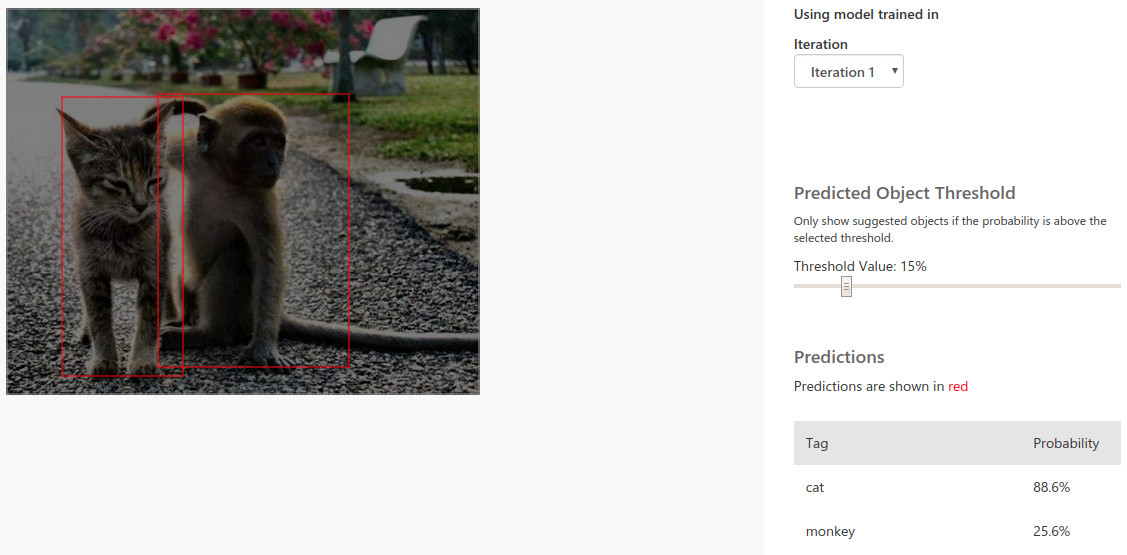
\includegraphics{image_report/monkey_cat_29.png}

    \begin{tcolorbox}[breakable, size=fbox, boxrule=1pt, pad at break*=1mm,colback=cellbackground, colframe=cellborder]
\prompt{In}{incolor}{25}{\boxspacing}
\begin{Verbatim}[commandchars=\\\{\}]
\PY{k+kn}{import} \PY{n+nn}{xml}\PY{n+nn}{.}\PY{n+nn}{etree}\PY{n+nn}{.}\PY{n+nn}{ElementTree} \PY{k}{as} \PY{n+nn}{ET}
\PY{c+c1}{\PYZsh{}tree = ET.parse(\PYZsq{}scripts/Data/PlayCards/AnnotationsTest/cam\PYZus{}image45.xml\PYZsq{})}
\PY{n}{tree} \PY{o}{=} \PY{n}{ET}\PY{o}{.}\PY{n}{parse}\PY{p}{(}\PY{l+s+s1}{\PYZsq{}}\PY{l+s+s1}{scripts/Data/monkeyCats/AnnotationsTest/cats\PYZus{}and\PYZus{}monkeys\PYZus{}029.xml}\PY{l+s+s1}{\PYZsq{}}\PY{p}{)}
\PY{n}{t\PYZus{}root} \PY{o}{=} \PY{n}{tree}\PY{o}{.}\PY{n}{getroot}\PY{p}{(}\PY{p}{)}
\PY{c+c1}{\PYZsh{}img = Image.open(\PYZsq{}scripts/Data/PlayCards/JPEGImagesTest/cam\PYZus{}image45.jpg\PYZsq{})}
\PY{n}{img} \PY{o}{=} \PY{n}{Image}\PY{o}{.}\PY{n}{open}\PY{p}{(}\PY{l+s+s1}{\PYZsq{}}\PY{l+s+s1}{scripts/Data/monkeyCats/JPEGImagesTest/cats\PYZus{}and\PYZus{}monkeys\PYZus{}029.jpg}\PY{l+s+s1}{\PYZsq{}}\PY{p}{)}
\PY{n}{draw} \PY{o}{=} \PY{n}{ImageDraw}\PY{o}{.}\PY{n}{Draw}\PY{p}{(}\PY{n}{img}\PY{p}{)}
\PY{k}{for} \PY{n}{obj} \PY{o+ow}{in} \PY{n}{t\PYZus{}root}\PY{o}{.}\PY{n}{findall}\PY{p}{(}\PY{l+s+s2}{\PYZdq{}}\PY{l+s+s2}{object}\PY{l+s+s2}{\PYZdq{}}\PY{p}{)}\PY{p}{:}
    \PY{n}{bnd\PYZus{}box} \PY{o}{=} \PY{n}{obj}\PY{o}{.}\PY{n}{find}\PY{p}{(}\PY{l+s+s2}{\PYZdq{}}\PY{l+s+s2}{bndbox}\PY{l+s+s2}{\PYZdq{}}\PY{p}{)}
    \PY{n}{xmin} \PY{o}{=} \PY{n+nb}{float}\PY{p}{(}\PY{n}{bnd\PYZus{}box}\PY{o}{.}\PY{n}{find}\PY{p}{(}\PY{l+s+s2}{\PYZdq{}}\PY{l+s+s2}{xmin}\PY{l+s+s2}{\PYZdq{}}\PY{p}{)}\PY{o}{.}\PY{n}{text}\PY{p}{)}
    \PY{n}{xmax} \PY{o}{=} \PY{n+nb}{float}\PY{p}{(}\PY{n}{bnd\PYZus{}box}\PY{o}{.}\PY{n}{find}\PY{p}{(}\PY{l+s+s2}{\PYZdq{}}\PY{l+s+s2}{xmax}\PY{l+s+s2}{\PYZdq{}}\PY{p}{)}\PY{o}{.}\PY{n}{text}\PY{p}{)}
    \PY{n}{ymin} \PY{o}{=} \PY{n+nb}{float}\PY{p}{(}\PY{n}{bnd\PYZus{}box}\PY{o}{.}\PY{n}{find}\PY{p}{(}\PY{l+s+s2}{\PYZdq{}}\PY{l+s+s2}{ymin}\PY{l+s+s2}{\PYZdq{}}\PY{p}{)}\PY{o}{.}\PY{n}{text}\PY{p}{)}
    \PY{n}{ymax} \PY{o}{=} \PY{n+nb}{float}\PY{p}{(}\PY{n}{bnd\PYZus{}box}\PY{o}{.}\PY{n}{find}\PY{p}{(}\PY{l+s+s2}{\PYZdq{}}\PY{l+s+s2}{ymax}\PY{l+s+s2}{\PYZdq{}}\PY{p}{)}\PY{o}{.}\PY{n}{text}\PY{p}{)}
    \PY{n}{label\PYZus{}name} \PY{o}{=} \PY{n+nb}{str}\PY{p}{(}\PY{n}{obj}\PY{o}{.}\PY{n}{find}\PY{p}{(}\PY{l+s+s2}{\PYZdq{}}\PY{l+s+s2}{name}\PY{l+s+s2}{\PYZdq{}}\PY{p}{)}\PY{o}{.}\PY{n}{text}\PY{p}{)}
    \PY{n}{draw}\PY{o}{.}\PY{n}{rectangle}\PY{p}{(}
            \PY{p}{(}\PY{p}{(}\PY{n}{xmin}\PY{p}{,} \PY{n}{ymin}\PY{p}{)}\PY{p}{,} \PY{p}{(}\PY{n}{xmax}\PY{p}{,} \PY{n}{ymax}\PY{p}{)}\PY{p}{)}\PY{p}{,} \PY{n}{outline}\PY{o}{=}\PY{l+s+s2}{\PYZdq{}}\PY{l+s+s2}{red}\PY{l+s+s2}{\PYZdq{}}
        \PY{p}{)}
    \PY{n}{draw}\PY{o}{.}\PY{n}{text}\PY{p}{(}\PY{p}{(}\PY{n}{xmin}\PY{p}{,} \PY{n}{ymin}\PY{p}{)}\PY{p}{,} \PY{n}{label\PYZus{}name}\PY{p}{,} \PY{n}{fill}\PY{o}{=}\PY{p}{(}\PY{l+m+mi}{255}\PY{p}{,}\PY{l+m+mi}{255}\PY{p}{,}\PY{l+m+mi}{255}\PY{p}{,}\PY{l+m+mi}{128}\PY{p}{)}\PY{p}{)}
\PY{n}{display}\PY{p}{(}\PY{n}{img}\PY{p}{)}
\end{Verbatim}
\end{tcolorbox}

    \begin{center}
    \adjustimage{max size={0.9\linewidth}{0.9\paperheight}}{image_report/output_66_0.png}
    \end{center}
    { \hspace*{\fill} \\}
    
    \hypertarget{wnioski-z-przykux142adu}) a małpa(\textbf{25.6\%}) prawdopodobieństwa,
natomiast dla Mask R-CNN dla kota jest prawie tak samo, natomiast małpa
wykryła się lepiej od Custom Vision.

\textbf{W tym wypadku Mask R-CNN pokazał siebie z lepszej strony}

    \hypertarget{oguxf3lne-wnioski-poruxf3wnanie}{%
\section{Ogólne wnioski \&
porównanie}\label{oguxf3lne-wnioski-poruxf3wnanie}}

    Wykrywanie obiektów to zadanie w wizji komputerowej, które obejmuje
identyfikację obecności, lokalizacji i typu jednego lub więcej obiektów
na danym zdjęciu.

Stworzyliśmy wytrenerowane modeli dla różnych typów danych (3 zbiory)
dla Mask R-CNN (Own model) oraz Azure Custom Vision.

\hypertarget{maska-r-cnn-do-wykrywania-obiektuxf3w}{%
\subsection{Maska R-CNN do wykrywania
obiektów}\label{maska-r-cnn-do-wykrywania-obiektuxf3w}}

Maska R-CNN - rozszerzenie szybszego R-CNN, które dodaje model wyjściowy
do przewidywania maski dla każdego wykrytego obiektu. 
\begin{itemize}
    \item  Maska R-CNN ma dodatkową gałąź do przewidywania masek segmentacji w każdym regionie zainteresowania (RoI) w sposób piksel-piksel
\end{itemize}


Model maski R-CNN jest podzielony na dwie części: 
\begin{itemize}
    \item  Sieć propozycji
regionów (RPN) do proponowania ramek ograniczających obiekty kandydatów.
\item  Binarny klasyfikator maski do generowania maski dla każdej klasy
\end{itemize}



\hypertarget{azure-custom-vision}{%
\subsection{Azure Custom Vision}\label{azure-custom-vision}}

\begin{itemize}
\tightlist
\item
  Custom Vision obsługuje następujące domeny do wykrywania obiektów:
  General, Logo, Products i Compact.
\item
  Szybka implementacja, dojść prosta w porównaniu do Mask R-CNN.
\end{itemize}

Azure Custom Vision to szybki i łatwy sposób tworzenia i wdrażania
modeli klasyfikacji i wykrywania obiektów. Portal internetowy umożliwia
eksperymentowanie ze zbiorem danych bez użycia kodu, ale jeśli chcemy
zaimplementować.Przesłaliśmy dane do Azure Custom Vision, następnie
wytrenowaliśmy model.

\hypertarget{poruxf3wnanie}{%
\subsection{Porównanie}\label{poruxf3wnanie}}

\textbf{Średni procent wykrywania (precyzja detektora obiektów w
znalezieniu)}

\begin{longtable}[]{@{}lll@{}}
\toprule
Dataset & MaskaR-CNN & Azure Custom Vision\tabularnewline
\midrule
\endhead
Fruit & 55\% - 80\% & 64\% - 97\%\tabularnewline
MonkeyCats & 49\% - 75\% & 91\% - 94\%\tabularnewline
PlayCards & 24\% - 54\% &\tabularnewline
\bottomrule
\end{longtable}

\textbf{Czas trwania}

\begin{longtable}[]{@{}lll@{}}
\toprule
Dataset & MaskaR-CNN & Azure Custom Vision\tabularnewline
\midrule
\endhead
Fruit & 1h 54m 18.30s &\tabularnewline
MonkeyCats & 3h 47m 4.478s &\tabularnewline
PlayCards & 2h 23m 4.841s &\tabularnewline
\bottomrule
\end{longtable}

Mask-RCNN to kolejna ewolucja modeli wykrywania obiektów, które
umożliwiają wykrywanie z większą precyzją. To tylko mały przykład tego,
co możemy osiągnąć dzięki temu wspaniałemu modelowi.

\hypertarget{plusy-azure-custom-vision}{%
\paragraph{Plusy Azure Custom Vision:}\label{plusy-azure-custom-vision}}

\begin{itemize}
\tightlist
\item
  Nie potrzebujemy dużo czasu, aby opracować algorytmy dla obrazu
\item
  Algorytmy będą ciągle optymalizowane i ewolucjowane przez analityka
  danych Microsoftu
\item
  Wysoka dokładność
\end{itemize}

\hypertarget{minusy-azure-custom-vision}{%
\paragraph{Minusy Azure Custom
Vision:}\label{minusy-azure-custom-vision}}

\begin{itemize}
\tightlist
\item
  Płatne
\item
  Nie wiemy, czy jest odpowiedni dla wszystkich sytuacji dla Klienta.
\item
  Ograniczenie się do algorytmów dostarczanych przez Microsoft i możemy
  zmobilizować bardzo niewiele parametrów do dopasowania modelu
\end{itemize}

Usługa platformy Azure jest tak użytecznym sposobem uczenia modelu
uczenia maszynowego, więc w tej usłudze nie ma się czego nie lubić.
Zdecydowanie polecamy innym korzystanie z usługi Azure Custom Vision.
Model możemy trenować po prostu klikając i nie wymagamy znajomości
algorytmów uczenia maszynowego.

Więc naszym zdaniem Azure Custom Vision jest lepszy!

\hypertarget{polecamy-microsoft-azure-custom-vision}{%
\section{Polecamy Microsoft Azure Custom Vision
!!!}\label{polecamy-microsoft-azure-custom-vision}}


\includegraphics{image_report/smile.jpeg}

    \begin{tcolorbox}[breakable, size=fbox, boxrule=1pt, pad at break*=1mm,colback=cellbackground, colframe=cellborder]
\prompt{In}{incolor}{ }{\boxspacing}
\begin{Verbatim}[commandchars=\\\{\}]

\end{Verbatim}
\end{tcolorbox}


    % Add a bibliography block to the postdoc
    
    
    
\end{document}